% !TeX program = LuaLaTeX
% !TeX spellcheck = en_US
% !TeX encoding = UTF-8

\documentclass[singlespacing]{lsuthesis}
% \documentclass[singlespacing,twoside,openright]{lsuthesis}  % Book printing
%% To experiment with using a different document class, such as the ``book'' class, comment-out the prior line and uncomment the next line.
%\documentclass[10pt,oneside]{book}
\hfuzz=0.25pt    % suppresses `Overfull \hbox` warnings

%% Specify additional LaTeX packages you need.
\usepackage[english]{babel}	   % English hyphenation
\usepackage{csquotes}    % Multilingual quotes
\usepackage[
    protrusion=true,
    expansion=true,
    final,
    babel,
]{microtype}    % Better typography
\usepackage{booktabs}    % Better tables
\usepackage[shortlabels]{enumitem}    % Better lists
\setlist{nosep}    % No separation between list items

% Graphics
\usepackage[
    svgnames,
    table,
    hyperref,
]{xcolor}
\usepackage{tikz}
\usetikzlibrary{cd}    % Commutative diagrams
\usetikzlibrary{patterns}
\usetikzlibrary{decorations.markings}

\usepackage{hyperxmp}    % eXtensible Metadata Platform
\usepackage{hyperref}
\hypersetup{%
    pdftitle = {Anticipating Stochastic Integrals and Related Linear Stochastic Differential Equations},
    pdfsubtitle={Doctoral Dissertation},
    pdfauthor={Sudip Sinha},
    pdfdate={2022-04-15},
    pdfcopyright={© 2022, Sudip Sinha},
    pdfsubject={anticipating stochastic calculus},
    pdfkeywords={dissertation, thesis, doctorate, PhD, anticipating stochastic calculus, anticipating stochastic integral, Ayed–Kuo integral, extension of Itô's isometry, near-martingale, optional stopping theorem, linear stochastic differential equation, conditioned process, large deviation principle},
    pdfcontactcountry={United States of America},
    pdfcontactphone={+1 754 666 0099},
    pdfcontactemail={sudipsinha@protonmail.com},
    pdfcontacturl={https://sites.google.com/view/sudip-sinha},
    pdflang={en-US},
    pdfmetalang={en-US},
    pdfpublication={LSU Doctoral Dissertations},
    pdfpublisher={Louisiana State University},
    pdfpubtype={book},
    pdfurl={https://digitalcommons.lsu.edu/cgi/viewcontent.cgi?article=6912\&context=gradschool\_dissertations},
    baseurl={https://digitalcommons.lsu.edu/gradschool_dissertations/5816/},
    pdffitwindow=true,    % resize document window to fit document size
    pdfstartview=FitBH,    % fits width of the page bounding box to the window - replace by FitH
    pdfpagelayout=OneColumn,    % one column; continuous scrolling
    colorlinks=true,
    linktoc=all,
    breaklinks=true,				% so long urls are correctly broken across lines
    linkcolor=Navy,
    urlcolor=IndianRed,
    citecolor=DarkSlateBlue,
}
\usepackage{pdfpages}
\usepackage[bottom]{footmisc}    % puts the footnote at the bottom of the page

% Indexing
\usepackage[symbols]{glossaries-extra}
\usepackage{makeidx}
\makeindex

% Reference management
\usepackage[
    style=alphabetic,
    sorting=nyt,
    backend=biber,
    maxnames=4,
]{biblatex}
\addbibresource{references/mypublications.bib}
\addbibresource{references/stochastics.bib}
\addbibresource{references/Wiener.bib}
\addbibresource{references/Kuo-integral.bib}
\addbibresource{references/Itô-integral.bib}
\addbibresource{references/large-deviations.bib}

% Unmarked footnotes for citations to published articles.
\makeatletter
\newcommand\footnotetextonly{\gdef\@thefnmark{}\@footnotetext}
\makeatother
% Alternative: No warnings, but weird spacing and no hyperlinks.
% \newcommand\footnotetextonly[1]{%
%   \begin{NoHyper}
%   \renewcommand\thefootnote{}\footnote{#1}%
%   \addtocounter{footnote}{-1}%
%   \end{NoHyper}
% }


\usepackage[parfill]{parskip}
% Single-spaced TOC
\usepackage[titles]{tocloft}    % `titles' start ToC at the top of the page
\renewcommand{\cftchapleader}{\cftdotfill{\cftdotsep}}    % Puts dots even for chapters
\renewcommand{\cftchapfont}{\rmfamily}    % Make chapter names not bold in Contents
\renewcommand{\cftchappagefont}{\rmfamily}    % Make chapter pages not bold in Contents


% Math
\usepackage[
    math-style=ISO,
    bold-style=ISO,
    ]{unicode-math}
\usepackage{amsthm}
% https://tex.stackexchange.com/questions/353266/dot-swap-numbers
% \usepackage{xpatch}
% \xpatchcmd\swappedhead{~}{.~}{}{}
% \swapnumbers    % `1 Theorem` instead of `Theorem 1`
\usepackage{cancel}    % Cancel in a oblique manner

% Fonts
\setmainfont{Stix Two Text}    % {Stix Two Text, XITS, GFSArtemisia}
\setmathfont{Stix Two Math}    % {Stix Two Math, XITS Math, texgyrepagella-math.otf}

% Referencing
\usepackage[noabbrev]{cleveref}    % Must be loaded last.

% Functions
\newcommand*{\floor}[1]{\ensuremath{\left\lfloor #1 \right\rfloor}}
\newcommand*{\ceil}[1]{\ensuremath{\left\lceil #1 \right\rceil}}
\newcommand*{\abs}[1]{\ensuremath{\left\lvert #1 \right\rvert}}
\newcommand*{\norm}[1]{\ensuremath{\left\lVert #1 \right\rVert}}
% Brackets
\newcommand*{\br}[1]{\ensuremath{\left( #1 \right)}}
\newcommand*{\bc}[1]{\ensuremath{\left\{ #1 \right\}}}
\newcommand*{\bs}[1]{\ensuremath{\left[ #1 \right]}}
\newcommand*{\ba}[1]{\ensuremath{\left\langle #1 \right\rangle}}
% Differentials
% \newcommand*{\dif}{\,\ensuremath{d}}
% \newcommand*{\Dif}{\,\ensuremath{D}}
% \newcommand*{\Del}{\,\ensuremath{Δ}}
\newcommand*{\dif}[1][]{\ensuremath{\operatorname{d}_{#1}\!}}
\newcommand*{\Dif}[1][]{\ensuremath{\operatorname{D}_{#1}\!}}
\newcommand*{\Del}[1][]{\ensuremath{\operatorname{Δ}_{#1}\!}}
% Miscellaneous
\renewcommand*{\Pr}{\ensuremath{ℙ\!}}
\newcommand*{\E}{\ensuremath{\operatorname{\mathbb{E}}\!}}
\newcommand*{\V}{\ensuremath{\operatorname{\mathbb{V}}\!}}
\newcommand*{\given}{\ensuremath{\; \middle| \;}}
\newcommand*{\inv}[1]{\ensuremath{{#1}^{-1}}}

% Environments
\numberwithin{equation}{section}

\theoremstyle{plain}
\newtheorem{theorem}[equation]{Theorem}
\newtheorem{lemma}[equation]{Lemma}
\newtheorem{proposition}[equation]{Proposition}
\newtheorem{corollary}[equation]{Corollary}

\theoremstyle{definition}
\newtheorem{definition}[equation]{Definition}
\newtheorem{hypothesis}[equation]{Hypothesis}
\newtheorem{example}[equation]{Example}

\theoremstyle{remark}
\newtheorem{remark}[equation]{Remark}
\newtheorem{question}[equation]{Question}



\usepackage{lsutitle}
\title{Anticipating Stochastic Integrals\\
and Related\\
Linear Stochastic Differential Equations}
% On capitalization, see Section 2.1.2 of https://www.ams.org/publications/authors/AMS-StyleGuide-online.pdf
\thesistype{Dissertation}
\department{The Department of Mathematics}
\soughtdegree{Doctor of Philosophy}
\author{Sudip Sinha}
\degrees{
    Bachelor of Engineering, Birla Institute of Technology and Science, Pilani, 2012\\
    Master of Science, MathMods, 2015\\
    Master of Science, Louisiana State University, 2018
}
\graduationdate{May 2022}



\begin{document}

%% The command ``\frontmatter'' switches to lowercase roman page numbers and unnumbered chapter headings without the word ``Chapter''.
\frontmatter

\maketitle


%% The following ``Copyright'' page is optional. You have inherent copyright on anything you create, even if you choose not to include a copyright notice. But if you choose to also formally register your copyright with the Library of Congress, then a centered copyright notice should follow the title page.
\begin{centeredpage}
© 2022\\
Sudip Sinha
\end{centeredpage}


%% The following ``Dedication'' page is optional.
\begin{centeredpage}
    % This dissertation is dedicated to Professor Fabio Antonelli, for if I had not met him, I would probably not have taken up research in mathematics.
    This dissertation is dedicated to Professor Fabio Antonelli. He is instrumental in leading me into the intriguing universe of mathematics. Had I not met him, I would probably not have taken up research in this discipline.
\end{centeredpage}


%% The following ``Epigraph'' page is optional.
\setlength{\epigraphwidth}{0.67\textwidth}
\begin{centeredpage}
    \epigraph{In precisely built mathematical structures, mathematicians find the same sort of beauty others find in enchanting pieces of music, or in magnificent architecture. There is, however, one great difference between the beauty of mathematical structures and that of great art. Music by Mozart, for instance, impresses greatly even those who do not know musical theory; the cathedral in Cologne overwhelms spectators even if they know nothing about Christianity. The beauty in mathematical structures, however, cannot be appreciated without understanding of a group of numerical formulae that express laws of logic. Only mathematicians can read \textquote{musical scores} containing many numerical formulae, and play that \textquote{music} in their hearts. Accordingly, I once believed that without numerical formulae, I could never communicate the sweet melody played in my heart. Stochastic differential equations, called \textquote{Itô Formula}, are currently in wide use for describing phenomena of random fluctuations over time. When I first set forth stochastic differential equations, however, my paper did not attract attention. It was over ten years after my paper that other mathematicians began reading my \textquote{musical scores} and playing my \textquote{music} with their \textquote{instruments}. By developing my \textquote{original musical scores} into more elaborate \textquote{music}, these researchers have contributed greatly to developing \textquote{Itô Formula}. In recent years, I find that my \textquote{music} is played in various fields, in addition to mathematics. Never did I expect that my \textquote{music} would be found in such various fields, its echo benefiting the practical world, as well as adding abstract beauty to the field of mathematics.}{— Kiyosi Itô \hspace*{16.75em} \\
    \textit{My Sixty Years along the Path of Probability Theory}}
\end{centeredpage}
    

\chapter{Acknowledgments}
% !TeX root = ../dissertation.tex

This dissertation results from a culmination of years of effort, help from many people, a robust support system, and love for knowledge. I would like to express heartfelt gratitude to my advisors — Professors Hui-Hsiung Kuo and Padmanabhan Sundar. Without their timely guidance, encouragement, patience, kindness, empathy, and unwavering support, I would not be where I am today. I shall strive to uphold the strong work ethic that I have witnessed in them. I would also like to thank Professors Ambar Sengupta and Gerry Knapp for serving on my advisory committee.

I am honored that Pujan Shrestha chose to work with me throughout the doctoral journey. Having a colleague with whom I could work in tandem made me cherish my time here. I am thankful to him for being patient with my mathematical ramblings, research discussions, and bringing me out of procrastination loops.

I am indebted to my master's thesis advisor Professor Fabio Antonelli. It is from him that I started to understand and appreciate mathematics for what it is. His teaching and advice motivated me to pursue research in stochastic analysis. I also want to thank Professors Davide Gabrielli, Ida Germana Minelli, and Prasanna Kumar for teaching me and supporting my endeavors. I am grateful to Professor Jeffrey Roland for helping me explore the foundations and philosophies of mathematics and to Professor James Oxley for helping me refine my communication techniques. I thank Professors Shipman, Adkins, Dasbach, and the other professors and graduate students for creating a lively and healthy environment conducive to research.

None of this would have been possible without a sturdy support system. I am grateful to my family for their unconditional love and support. I would like to thank Bree, Kaju, Jessica, Rachel, Steven, Irfan, Liem, Huy, and all my friends who made living in Baton Rouge an enjoyable experience. My heartfelt gratitude to Ankan and Anirudh for lively discussions on mathematics, the universe, and everything. I am grateful to Tuppu for being a constant source of love, support, and inspiration.

Finally, my work builds on the mathematical framework laid by mathematicians and philosophers over millennia of painstaking effort. Quoting Isaac Newton, \textquote{If I have seen further, it is by standing on the shoulders of giants.}


% The `group` creates a local environment for link colors.
\begingroup
\hypersetup{linkcolor=black}
\tableofcontents
\endgroup

% % The list of tables is optional. Remove the following line if you don't have tables, don't have many tables, or simply don't wish to have a list of tables.
% \listoftables

% % The list of figures is optional. Remove the following line if you don't have figures, don't have many figures, or simply don't wish to have a list of figures.
% \listoffigures

% \chapter{Nomenclature, Symbols, Acronyms}
% The ``nomenclature, symbols, acronyms'' page is optional.

\chapter{Abstract}
% !TeX root = ../dissertation.tex

Itô’s stochastic calculus revolutionized the field of stochastic analysis and has found numerous applications in a wide variety of disciplines. Itô’s theory, even though quite general, cannot handle anticipating stochastic processes as integrands. There have been considerable efforts within the mathematical community to extend Itô’s calculus to account for anticipation. The Ayed–Kuo integral — introduced in 2008 — is one of the most recent developments. It is arguably the most accessible among the theories extending Itô’s calculus — relying solely on probabilistic methods. In this dissertation, we look at the recent advances in this area, highlighting our contributions. First, we extend the class of linear stochastic differential equations with anticipating initial conditions that have closed-form solutions in this theory. Then we prove an extension of Itô’s isometry for the Ayed–Kuo integral using purely probabilistic tools and exploiting the intrinsic nature of the integral. We also prove an optional stopping theorem for near-martingales — the counterpart of martingales in the Ayed–Kuo theory. We study the behavior of conditioned processes corresponding to the solution of a linear stochastic differential equation with anticipating initial conditions. We analyze a particular class of linear stochastic differential equations with anticipating coefficients in the drift term and derive the solution using two methods: (1) by guessing an ansatz and using the general differential formula in the Ayed–Kuo theory, and (2) by introducing a novel \textquote{braiding} technique that allows us to construct the solution by an iterative process. We derive explicit solutions in each theory independently and show that both methods yield the same solution under identical conditions. We establish a Freidlin–Wentzell type large deviations principle for solutions of this specific class of anticipating linear stochastic differential equations. Finally, we highlight a few areas of research in this field.




%% The command ``\mainmatter'' switches to regular page numbers and chapter headings that include the word ``Chapter''.
\mainmatter

\chapter{Introduction}
\label{chp:introduction}
% !TeX root = ../dissertation.tex

In 1827, while examining pollen grains suspended in water under a microscope, the British botanist Robert Brown observed that minute particles ejected from the pollens executed a continuous jittery motion\cite{Brown1828}. Since he observed the same kind of motion in inanimate objects like dust particles, he concluded that the motion was not related to life. He did not provide a theory to explain the phenomenon. However, this seemingly random motion came to be known as Brownian motion.

Surprisingly, Brownian motion did not get a lot of attention for more than half a century. In 1900, Louis Bachelier used Brownian motion in his PhD thesis \textquote{The theory of speculation}\cite{Bachelier1900}, where he presented a stochastic analysis of stock and option markets. The phenomenon gained a lot of attention again in 1905 when Albert Einstein presented an indirect method to verify the existence of atoms and molecules in one of his papers\cite{Einstein1905}. Around the same time, in 1902, Henri Lebesgue laid the foundation of measure theory and abstract integration theory\cite{Lebesgue1902}.

\begin{figure}[h]
    \centering
    \begin{tikzpicture}[domain=0:10]
        % https://tex.stackexchange.com/questions/59926/how-to-draw-brownian-motions-in-tikz-pgf
        \pgfmathsetseed{2}
        \tikzset{help lines/.style={very thin,color=Linen}}
        \newcommand{\BrownianPath}[5]{% points, advance, rand factor, options, end label
            \draw[#4] (0,0)
            \foreach \x in {1,...,#1} {
                -- ++(#2,rand*#3)
            }
            node[right] {#5};
        }

        \draw[help lines] (0,-2.5) grid (9.5,2.5);

        \BrownianPath{1000}{0.01}{0.1}{PaleVioletRed}{\( W_⋅(ω_1) \)};
        \BrownianPath{1000}{0.01}{0.1}{DarkSlateBlue}{\( W_⋅(ω_2) \)};
        \BrownianPath{1000}{0.01}{0.1}{YellowGreen}{\( W_⋅(ω_3) \)};
        \BrownianPath{1000}{0.01}{0.1}{DarkSalmon}{\( W_⋅(ω_4) \)};
        \BrownianPath{1000}{0.01}{0.1}{Crimson}{\( W_⋅(ω_5) \)};
        \BrownianPath{1000}{0.01}{0.1}{Fuchsia}{\( W_⋅(ω_6) \)};
        \BrownianPath{1000}{0.01}{0.1}{Coral}{\( W_⋅(ω_7) \)};

        \draw[->] (0, 0) -- (10, 0) node[right] {\( t \)};
        \draw[->] (0, -3) -- (0, 3) node[right] {\( x \)};
    \end{tikzpicture}
    \caption{Some paths of a Wiener process.}
    \label{fig:Wiener_process_paths}
\end{figure}

However, there was no mathematical description of this phenomenon until this point. In 1923, the American mathematician Norbert Wiener showed how Brownian motions can be constructed in a mathematical sense by putting an appropriate measure on the space of continuous functions\cite{Wiener1923}, which is arguably the first really significant application of abstract measure theory. Note that this was a decade before Andreĭ Nikolaevich Kolmogorov laid the rigorous foundations of probability theory\cite{Kolmogorov1933}. Therefore, the stochastic process corresponding to Brownian motion process is popularly known as Wiener process in mathematics. Wiener also constructed an integral with respect to Wiener processes. We shall explore this idea in \cref{sec:Wiener_integral}.

Wiener's integral allowed only integration of deterministic functions. In 1944, Kiyosi Itô published his seminal paper \textquote{Stochastic Integral}\cite{Itô1944SI}, in which he demonstrated how to integrate adapted stochastic processes. In layperson's terms, adapted processes are processes that can utilize information only until the present. Itô calculus forms the counterpart to the Leibniz–Newton calculus for random processes. Itô combined the ideas of the Riemann–Stieltjes integral (referring to the integrator) and the Lebesgue integral (referring to the integrand). This will be the focus of much of \cref{chp:introduction}, starting from \cref{sec:Itô_integral}.

Since its inception, Itô's theory has been used in numerous scientific pursuits. One of the biggest achievements is the Black–Scholes–Merton model\cite{BS1973,Merton1974}, which is an application of Itô's calculus to model the dynamics of financial markets. Merton and Scholes received the 1997 Nobel Memorial Prize in Economic Sciences. Due to his death in 1995, Black was mentioned as a contributor but was not named as an awardee.

Itô's theory, even though quite general and useful, is not applicable to certain circumstances. For example, one cannot integrate \textquote{anticipating} processes, or processes that can have access to the future. Therefore, one cannot model insider trading using Itô's calculus. Similarly, if one knows the probability distribution of a road network being repaired at a certain future date and wants to model the logistics of delivering goods, the resulting model would fall outside the scope of Itô's theory.

There have been many attempts at enlarging the space of integrable stochastic processes. Some classic approaches are (1) enlargement of filtration due to Itô himself, (2) the Skorokhod integral and Malliavin calculus, (3) white noise distribution theory, and (4) the more recent Ayed–Kuo integral. In this dissertation, we mainly focus on the Ayed–Kuo integral. We look at the current state of research in this area. We also prove large deviation principles for anticipating linear stochastic differential equations defined in the Ayed–Kuo sense.

\begin{figure}[ht]
    \centering
    \begin{tikzcd}[row sep=huge, column sep=huge, math mode=false, crossing over clearance=0.5ex]
        & & \ref{chp:introduction}
        \arrow[d  , bend right, ForestGreen]
        \arrow[dd , bend left , ForestGreen]
        \\
        & &
        \ref{chp:extensions}
        \arrow[d  , bend right, ForestGreen]
        \arrow[ddr, bend right=6,  densely dotted, IndianRed]
        \\
        & &
        \ref{chp:Ayed–Kuo_integral}
        \arrow[dll, crossing over, bend right=15 , ForestGreen]
        \arrow[dl , crossing over, bend right=6  , ForestGreen]
        \arrow[d  , crossing over, ForestGreen]
        \arrow[dr , bend left=6  , ForestGreen]
        \arrow[drr, bend left=15 , ForestGreen]
        \\
        \ref{chp:isometry}
        &
        \ref{chp:near-martingales}
        &
        \ref{chp:conditional}
        &
        \ref{chp:solving_ALSDEs}
        \arrow[r  , bend left=6  , densely dotted , IndianRed]
        &
        \ref{chp:probabilistic_behavior}
    \end{tikzcd}
    \caption{Chapter dependency graph. Dotted lines represent partial dependency.}
    \label{fig:chapter_dependency_graph}
\end{figure}

This document is organized as follows. \Cref{chp:introduction} introduces elementary ideas, martingales, stochastic integration, and stochastic differential equations. \Cref{chp:extensions} discusses some mathematical motivations to extend Itô's calculus to a anticipating integrands, and a brief overview of the various approaches that have been taken in this direction. \Cref{chp:Ayed–Kuo_integral} introduces the Ayed–Kuo integral, the central theme of this dissertation. In \cref{chp:isometry}, we prove an extension of Itô's isometry for Ayed–Kuo integrals. In \cref{chp:near-martingales}, we introduce near-martingales, and prove an optional stopping theorem that we use in \cref{chp:probabilistic_behavior}. In \cref{chp:conditional}, we discuss how conditionals of solutions of stochastic differential equations behave. In \cref{chp:solving_ALSDEs}, we focus on a particular class of stochastic differential equations and contrast different techniques to solve them. We also discuss existence and uniqueness results. In \cref{chp:probabilistic_behavior}, we derive Freidlin–Wentzell type large deviation principles for the class of stochastic differential equations discussed in \cref{chp:solving_ALSDEs}. Finally, in \cref{chp:epilogue}, we conclude by looking at useful examples and open problems that need to be addressed.

In general, the document is designed to be read linearly. \Cref{chp:extensions} can be skipped for the Ayed–Kuo part starting on \cref{chp:Ayed–Kuo_integral}. However, the ideas of enlargement of filtration and Skorokhod integral (\cref{sec:Malliavin_calculus}) of \cref{chp:extensions} are required for the corresponding sections in \cref{chp:solving_ALSDEs}. \Cref{chp:isometry,chp:near-martingales,chp:conditional} are independent and can be read after \cref{chp:Ayed–Kuo_integral}. The dependency graph of the chapters is shown in \cref{fig:chapter_dependency_graph}. \Cref{chp:probabilistic_behavior} uses results from \cref{chp:solving_ALSDEs}, but is independent in essence. \Cref{chp:epilogue} is independent in spirit, though it refers to various results shown in the other chapters for context. See \cref{fig:chapter_dependency_graph} for a dependency graph.



\section{Elementary ideas and notation}
A \emph{probability space}\index{probability space} is a triple \( (Ω, Σ, \Pr ) \) such that
\begin{enumerate}
    \item  \( Ω \) is a set.
    \item  \( Σ \) is a \emph{σ-algebra}\index{sigma@σ-algebra} on \( Ω \). This means \( Σ ⊆ 2^Ω \) such that
        \begin{enumerate}
            \item  \( ∅ ∈ Σ \),
            \item  \( E ∈ Σ \) implies \( E^∁ ∈ Σ \), and
            \item  for every countable family of sets \( \br{E_n}_{n = 1}^∞ \) in \( Σ \), the union \( ⋃ E_n ∈ Σ \).
        \end{enumerate}
    \item   \( \Pr: Σ → [0, 1] \) is a \emph{probability measure}\index{probability measure}, that is
        \begin{enumerate}
            \item  \( \Pr\br{Ω} = 1 \), and
            \item  if \( \br{E_n}_{n = 1}^∞ ⊆ Σ \) is a mutually disjoint collection of sets, then \( \Pr\br{⨆ E_n} = ∑ \Pr\br{E_n} \).
        \end{enumerate}
\end{enumerate}

We usually think of a σ-algebra as the available information regarding the system of concern. A σ-algebra is called \emph{complete}\index{sigma@σ-algebra!complete} if all subsets of zero-measure sets are also measurable. In this document, we assume that all σ-algebras are complete. The σ-algebra generated by a topology is called \emph{Borel σ-algebra}\index{sigma@σ-algebra!Borel}. Sometimes we suppress the filtration and write the probability space as \( (Ω, \Pr) \) if the σ-algebra is the Borel σ-algebra. Elements of \( Σ \) are called \emph{events}\index{events}. We say that an event \( E \) occurs \emph{almost surely}\index{almost surely} if \( \Pr\br{E} = 1 \).

A \emph{random variable}\index{random variable} \( X \) is a \emph{measurable}\index{measurable} function from a probability space \( (Ω, Σ, \Pr) \) to the reals embedded with the Borel σ-algebra. That is, for every \( B ∈ ℬ \), the set \( \bc{X ∈ B} = X^{-1}(B) ∈ Σ \). A random variable is called \emph{integrable}\index{random variable!integrable} if \( ∫ \abs{X} \dif \Pr < ∞ \). The \emph{expectation}\index{expectation} of an integrable random variable \( X \) is defined as the integral \( \E\br{X} = ∫_Ω X \dif \Pr \).

In order to model random phenomenon evolving in time, we define stochastic processes.
A \emph{stochastic process}\index{stochastic process} is a function \( X: 𝕋 × Ω → ℝ \) such that
\begin{enumerate}
    \item  \( X(t, ⋅): Ω → ℝ \) is a random variable for each \( t ∈ 𝕋 \), and
    \item  \( X(⋅, ω): 𝕋 → ℝ \) is measurable for each \( ω ∈ Ω \).
\end{enumerate}
Stochastic processes are essentially families of random variables indexed by \( t ∈ 𝕋 \). We think of the parameter \( t \) as representing time. We usually suppress the dependence on \( ω ∈ Ω \) and simply write \( X(t) \) or \( X_t \). The space \( (ℝ, ℬ) \) is called the \emph{state space} and \( 𝕋 \) the \emph{index set}. For a fixed \( ω \), the function \( X(⋅, ω): 𝕋 → ℝ \) is called a \emph{path} of the process. We only consider the case where the \( 𝕋 = [a, b] \), where \( a, b ∈ ℝ \) and \( a < b \). A stochastic process \( X \) is said to be \emph{integrable}\index{stochastic process!integrable} if the random variable \( X_t \) is integrable for each \( t \).

We now present an axiomatic definition of a Wiener process — which shall be the focal point of this document.
\begin{definition}  \label{def:Wiener_process}  \index{Wiener process}  \index{Brownian motion}
    A stochastic process \( W = \br{W_t}_{t ≥ 0} \) is called a \emph{Wiener process} or \emph{Brownian motion} if
    \begin{enumerate}
        \item  \( W_0 = 0 \) a.s.
        \item  \( W \) has independent increments: for every \( 0 ≤ t_1 ≤ \dotsb ≤ t_n \), the random variables \( W_{t_1}, W_{t_2} - W_{t_1}, \dotsc, W_{t_n} - W_{t_{n - 1}} \) are independent.
        \item  \( W \) has Gaussian increments: \( W_t - W_s ∼ N(0, \abs{t - s}) \) for any \( s \) and \( t \).
        \item  The paths of \( W \) are almost surely continuous in \( t \).
    \end{enumerate}
\end{definition}

\begin{theorem}[{\cite[theorem 2.2.5]{KallianpurSundar2014}}]  \label{thm:Wiener_process_nowhere_differentiable}
    The paths of a Wiener process are almost surely nowhere differentiable.
\end{theorem}


Often, we want to know the expected value of a process given restricted information. This is achieved by using conditional expectation. Suppose \( ℱ ⊆ Σ \) is a sub-σ-algebra, and \( X \) is an integrable random variable. Then the \emph{conditional expectation}\index{conditional expectation} of \( X \) given \( ℱ \), denoted \( \E\br{X \given ℱ} \) is a \( ℱ \)-measurable random variable \( Y \) such that \( ∫_E Y \dif \Pr = ∫_E X \dif \Pr \) for any \( E ∈ ℱ \).

\begin{theorem}[properties of conditional expectation]  \label{thm:conditional_expectation_properties}
    Let \( X, Y \) be random variables, \( a, b \) scalars, and \( 𝒢 ⊆ ℱ ⊆ Σ \) σ-algebras. Then under suitable integrability conditions, the following hold almost surely.
    \begin{enumerate}
        \item  Mean-preserving: \( \E\br{\E\br{X \given ℱ}} = \E\br{X} \).
        \item  Linearity: \( \E\br{a X + b Y \given ℱ} = a \E\br{X \given ℱ} + b \E\br{Y \given ℱ} \).
        \item  Monotonicity: If \( X ≥ 0 \), then \( \E\br{X \given ℱ} ≥ 0 \).
        \item  Taking out the known: If \( Y \) is \( ℱ \)-measurable, then \( \E\br{X Y \given ℱ} = Y \E\br{X \given ℱ} \).
        \item  Independence: If \( 𝒢 \) is independent of \( σ\bc{σ(X), ℱ} \), then \( \E\br{X \given σ(ℱ, 𝒢)} = \E\br{X \given ℱ} \). In particular, if \( X \) is independent of \( ℋ \), then \( \E\br{X \given 𝒢} = \E\br{X} \).
        \item  Tower property: \( \E\br{\E\br{X \given ℱ} \given 𝒢} = \E\br{X \given 𝒢} \).
    \end{enumerate}
\end{theorem}
For the proof of the above, see \cite[section 9.7]{Williams1991}.


An non-decreasing indexed family of σ-algebras \( ℱ = (ℱ_t)_{t ∈ 𝕋} \), is called a \emph{filtration}\index{filtration}. A probability space embedded with a filtration is called a \emph{filtered probability space}\index{filtered probability space} and is denoted by \( (Ω, Σ, ℱ, \Pr) \). A filtration is said to be \emph{right-continuous}\index{filtration!right-continuous} if \( ℱ_{t^+} = ℱ_t \), where \(ℱ_{t^+} = ⋂_{u > t} ℱ_u \). A filtered probability space is said to satisfy the \emph{usual conditions}\index{filtered probability space!usual conditions} if the associated filtration is complete and right-continuous. In the information interpretation, a filtered probability space represents the temporal evolution of knowledge about the system. We refer to the filtration generated by the relevant Wiener process as the \emph{natural filtration}\index{natural filtration}.

\begin{definition}  \index{adapted}
    A stochastic process \( A \) is called \emph{\( ℱ \)-adapted} if \( A_t \) is \( ℱ_t \)-measurable for every \( t \). If the σ-algebra is obvious, we simply say \emph{adapted}.
\end{definition}

A Wiener process is trivially adapted to its natural filtration.

Now, we define stopping times.
\begin{definition}
    A stochastic process \( τ \) is called a \emph{stopping time}\index{stopping time} if \( \bc{τ ≤ t} ∈ ℱ_t \) for every \( t \). The σ-algebra at a stopping time \( τ \)\index{sigma@σ-algebra!stopped} is defined as
    \[ ℱ_τ = \bc{E ∈ Σ \given E ∩ \bc{τ ≤ t} ∈ ℱ_t \text{ for all } t} . \]
\end{definition}

A process \textquote{stopped} using a stopping time has a constant value after it is stopped.
\begin{definition}
    Suppose \( X \) is a stochastic process and \( τ \) is a stopping time. Then the \emph{stopped process}\index{stopped process} \( X^τ \) is defined by
    \[ X^τ_t(ω) = X_{τ(ω) ∧ t}(ω) , \]
    where we use the notation \( a ∧ b = \min\bc{a, b} \).
\end{definition}

\paragraph{Conventions}
In this document, unless specified, we fix the following.
\begin{enumerate}
    \item  An underlying filtered space \( (Ω, Σ, ℱ, \Pr) \) satisfying the usual conditions.
    \item  The interval of interest of the parameter \( t \) is \( 𝕋 = [a, b] \), where \( 0 ≤ a ≤ b < ∞ \).
    \item  A Wiener process \( W = \br{W_t}_{t ≥ 0} \).
    \item  The natural filtration as the reference filtration.
\end{enumerate}




\section{Martingales}  \label{sec:martingales}

\begin{definition}  \index{martingale}  \index{submartingale}  \index{supermartingale}
    An integrable adapted stochastic process \( M \) is called a \emph{martingale} if \( \E\br{M_t \given ℱ_s} = M_s \) for every \( s ≤ t \). It is called a \emph{submartingale} if we replace the condition with \( \E\br{M_t \given ℱ_s} ≥ M_s \), and is called a \emph{supermartingale} when \( \E\br{M_t \given ℱ_s} ≤ M_s \).
\end{definition}

From a modeling perspective, the best predictor of the future value of a martingale is its present value. Therefore, martingales are used to model fair games and find numerous application in pricing financial products.

A process that is both a submartingale and a supermartingale is necessarily a martingale. Moreover, any result that is true for a submartingale can be suitably modified for a supermartingale, and subsequently for a martingale. Therefore, in what follows, we only show results for submartingales.

Let us look at some examples of martingales.
\begin{enumerate}
    \item  Suppose \( \br{X_n}_{n = 1}^∞ \) is a sequence of integrable independent zero-mean random variables. Let \( S_n = ∑_{i = 1}^n X_i \). Then \( S \) is a martingale.
    \item  Suppose \( \br{X_n}_{n = 1}^∞ \) is a sequence of integrable, independent and identically distributed (i.i.d.) random variables with zero mean and unit variance, and \( S_n = ∑_{i = 1}^n X_i \). Then \( S_n^2 - n \) is a martingale.
    \item  If \( ξ \) is integrable, then the process \( M_t = \E\br{ξ \given ℱ_t} \) is a martingale.
    \item  A Wiener process \( W \) is a martingale.
        \begin{proof}
            Suppose \( s ≤ t \). We write \( W_t = W_s + (W_t - W_s) \). By independence of increments, we know \( W_t - W_s \) is independent of \( ℱ_s \). Moreover, \( \E\br{W_t - W_s} = 0 \). Using \cref{thm:conditional_expectation_properties}, we get
            \( \E\br{W_t \given ℱ_s}
                =  \E\br{W_s \given ℱ_s} + \E\br{W_t - W_s \given ℱ_s}
                =  W_s + \cancelto{0}{\E\br{W_t - W_s}}
                =  W_s \).
        \end{proof}
    \item  The processes \( W_t^2 - t \) and \( W_t^3 - 3t W_t \) are martingales.
    \item  \( \exp\br{W_t^2 - \frac12 t} \) is a martingale.
\end{enumerate}

Since the expected value of a submartingale increases, it is natural to ask if we can decompose it into a martingale and an increasing process. The following theorem answers this question.
\begin{theorem}[Doob–Meyer decomposition]  \index{Doob–Meyer decomposition}
    Suppose \( X \) is a integrable adapted process. Then there is a unique decomposition
    \begin{equation*}
        X_t = M_t + A_t \quad \text{for all } t ,
    \end{equation*}
where \( M \) is a martingale and \( A \) is a adapted integrable process.
\end{theorem}

\begin{theorem}[Doob–Meyer decomposition for submartingales]  \label{thm:Doob–Meyer_decomposition_submartingales}  \index{Doob–Meyer decomposition!submartingales}
    Suppose \( X \) is a submartingale. Then there is a unique decomposition
    \begin{equation*}
        X_t = M_t + A_t \quad \text{for all } t ,
    \end{equation*}
where \( M \) is a martingale and \( A \) is a adapted integrable increasing process starting at \( 0 \).
\end{theorem}


The power of martingales come from martingale transforms. We think of this as follows. Imagine a discrete-time game of chance, where the difference \( X_n - X_{n-1} \) is our winning per unit stake at time \( n ≥ 1 \). At time \( 0 \), we place a random stake \( A_0 \) using our prior intuition. Our winning at time \( 1 \) is then \( A_0 (X_1 - X_0) \). At time \( 1 \), we update our prior to the present and place stake \( A_1 \) to get a winning of \( A_1 (X_2 - X_1) \) at time \( 2 \). Therefore, the net gain until time \( 2 \) is \( ∑_{i = 1}^2 A_{n-1} (X_n - X_{n-1}) \). In general, at time \( n \), our portfolio value would be \( ∑_{i = 1}^n A_{n-1} (X_n - X_{n-1}) \). This is the motivation behind the following definition.

\begin{definition}  \index{martingale transform}
    Let \( \br{A_n}_{n = 0}^∞ \) be an adapted process and \( \br{X_n}_{n = 0}^∞ \) a submartingale. Then the processes \( \br{Y_n}_{n = 0}^∞ \), where \( Y_0 = 0 \) and
    \begin{equation*}
        Y_n = (A ∙ X)_n = ∑_{i = 1}^n A_{n-1} (X_n - X_{n-1})
    \end{equation*}
    is called the \emph{martingale transform} of \( X \) by \( A \).
\end{definition}

Note that we required \( A \) to be adapted so that the bets are fair in the sense that one does not know the result of the lottery at any future time. Since we have no information of the future, if the underlying game is fair (martingale), no matter how we bet, we should neither win nor lose in expectation. This is what we now show.

\begin{proposition}  \label{thm:martingale_transform}
    \begin{enumerate}
        \item \label{itm:martingale_transform_bounded_positive}  If \( X \) is a submartingale and \( A \) is a bounded non-negative adapted process, then \( (A ∙ X) \) is a submartingale.
        \item \label{itm:martingale_transform_bounded}  If \( X \) is a martingale and \( A \) is a bounded adapted process, then \( (A ∙ X) \) is a martingale.
        \item  If \( X \) and \( A \) are both square integrable, then we do not require the boundedness condition in \cref{itm:martingale_transform_bounded_positive,itm:martingale_transform_bounded}.
    \end{enumerate}
\end{proposition}
\begin{proof}
    We only prove \cref{itm:martingale_transform_bounded_positive} because the others follow the same process. Let \( X \) be a submartingale and \( Y = (A ∙ X) \). Suppose \( n \) is an arbitrary time. Note that \( Y_n - Y_{n-1} = A_{n-1} (X_n - X_{n-1}) \), which is integrable since \( A \) is bounded. Using the adaptedness of \( A \), we get
    \begin{equation*}
        \E\br{Y_n - Y_{n-1} \given ℱ_{n-1}}
        =  \E\br{A_{n-1} (X_n - X_{n-1}) \given ℱ_{n-1}}
        =  A_{n-1} \E\br{X_n - X_{n-1} \given ℱ_{n-1}}
        ≥  0 ,
    \end{equation*}
    where the last inequality holds since \( A \) is non-negative.
\end{proof}

Given a martingale, one can expect that the martingale property is preserved when sampling on stopping times. This always holds \cite[for the discrete case, see][page 99]{Williams1991}. However, it is not always true that the expected value of the stopped process is the same as the expected value at the initial time. For example, let \( X \) be a simple random walk on the natural numbers (including \( 0 \)) starting at \( 0 \) and let \( τ = \inf\bc{X_n = 1} \). Then \( X \) is a martingale and it is well-known that \( ℙ(T < ∞) = 1 \). However, even though \( \E\br{X_{τ ∧ n}} = \E\br{X_0} \) for every \( n \), we have \( 1 = \E\br{X_τ} ≠ \E\br{X_0} = 0 \). Doob's optional stopping theorem\index{optional stopping theorem!martingale} states that this is true under reasonable conditions. 
\begin{theorem}[{\cite[theorem 3.3.1]{KallianpurSundar2014}}]  \label{thm:optional_stopping_Doob}
    Let \( M \) be a uniformly integrable submartingale with right-continuous sample paths. Suppose \( σ \) and \( τ \) are two bounded stopping times with \( σ ≤ τ \). Then \( M_σ \) and \( M_τ \) are integrable, and \( \E\br{X_τ \given ℱ_σ} ≥ X_σ \) almost surely.
\end{theorem}



\section{Naively approaching stochastic integration}
Our goal in this section is to define integrals with respect to Wiener processes. That is, we want to define \( ∫_a^b f(t) \dif W_t \). Can we do so in the usual Riemann–Stieltjes sense?

A set \( Π_n = \bc{t_0, t_1, \dotsc, t_n} \), is called a \emph{partition}\index{partition} of \( [a, b] \) if \( a = t_0 < t_1 < \dotsb < t_n = b \). We define the norm of a partition as \( \norm{Π_n} = \sup \bc{t_i - t_{i-1} \given i ∈ [n]} \). In this document, we always assume \( \norm{Π_n} → 0 \) as \( n → ∞ \).

We first introduce the idea of variations of a real-valued function \( f \). 
\begin{definition}
    The \emph{linear variation}\index{variation!linear} of a function \( f: [a, b] → ℝ \) is the quantity
    \[ L_a^b(f) = \sup_{Π_n} ∑_{i = 0}^n \abs{f(x_i) - f(x_{i - 1})} , \]
    where the supremum is taken over all partitions of \( [a, b] \).

    Similarly, the \emph{quadratic variation}\index{variation!quadratic} of a function \( f: [a, b] → ℝ \) is the quantity
    \[ Q_a^b(f) = \sup_{Π_n} ∑_{i = 0}^n \abs{f(x_i) - f(x_{i - 1})}^2 . \]
\end{definition}

It can easily be checked that the quadratic variation of a Wiener process is given by
\begin{equation}  \label{eqn:quadratic_variation_W}
    Q_a^b(W) = b - a ,
\end{equation}
which we symbolically denote by \( \br{\Del W_i}^2 ≃ \Del t_i \).

Now, suppose \( \norm{Π_n} → 0 \) as \( n → ∞ \). Then the Riemann–Stieltjes integral for \( f \) with respect to \( g \) is defined as
\[ ∫_a^b f(t) \dif g(t)  =  \lim_{n → ∞} ∑_{i = 1}^n f(t_i^*) \br{g(t_i) - g(t_{i-1})} , \]
where \( t_i^* ∈ [t_{i-1}, t_i] \) for \( i ∈ [n] = \bc{1, 2, \dotsc, n} \).
It can be shown that continuous functions are Riemann–Stieltjes integrable with respect to any function of finite linear variation.

Can we use this idea to define \( ∫_a^b f(t) \dif W_t \) for a continuous function \( f \)? Since the linear variation of a Wiener process over any interval is infinite, we cannot define path-wise a stochastic integral of the form \( ∫_a^b f(t) \dif W_t( ω) \). In other words, naive integration with respect to a Wiener process is not possible.



\section{Wiener's integral}  \label{sec:Wiener_integral}
As we remarked in \cref{eqn:quadratic_variation_W}, Wiener processes have finite quadratic variations. Can we exploit this fact to define an integral with respect to Wiener processes?

Wiener\cite{Wiener1923} did exactly this for square-integrable deterministic functions \( f ∈ L^2[a, b] \). His approach was to first define the integral on \emph{step functions}\index{step function}. In particular, for \( f(t) = ∑_{i = 1}^n a_i 𝟙_{[t_{i-1}, t_i)}(t) \), define the \emph{Wiener integral}\index{integral!Wiener} as
\[ I_W(f) = ∑_{i = 1}^n a_i \Del W_i , \]
where \( \Del W_i = W_{t_i} - W_{t_{i-1}} \).
In order to extend this idea to \( L^2[a, b] \), we note that step functions are dense in the space of square integrable functions. Therefore, for any \( f ∈ L^2[a, b] \), we can find a sequence of functions \( \br{f^{(n)}}_{n = 1}^∞ \) such that \( f^{(n)} → f \) in \( L^2[a, b] \) as \( n → ∞ \). It can be shown that \( \br{I(X^{(n)})}_{n = 1}^∞ \) is a Cauchy sequence in \( L^2(Ω) \). Since \( L^2(Ω) \) is a Hilbert space, the sequence \( \br{I(f^{(n)})}_{n = 1}^∞ \) converges in \( L^2(Ω) \). We call this limit as the Wiener integral of \( f \), and write
\[ I_W(f) = ∫_a^b f(t) \dif W_t = \lim_{n → ∞} ∫_a^b f^{(n)}(t) \dif W_t . \]

The Wiener integral is linear and retains the Gaussian nature of Wiener processes. In particular,
\[ I_W(f) ∼ N\br{0, \norm{f}} , \]
where \( \norm{f}^2 = ∫_a^b f(t)^2 \dif t \) is the canonical norm on \( L^2[a, b] \). Moreover, the process \( X \) defined by \( X_t = ∫_a^t f(s) \dif W_s \) is a continuous martingale.



\section{Itô's integral}  \label{sec:Itô_integral}  \index{integral!Itô}
Itô generalized Wiener's integral to allow integrands to be adapted stochastic processes, thus expanding the class of integrable functions significantly \cite{Itô1944SI}. Itô's original motivation was to construct diffusion processes associated with infinitesimal operators directly in a probabilistic manner. However, we take a martingale viewpoint in this dissertation. To understand a motivation of his definition, we first try to compute the integral of a Wiener process with respect to itself. Writing as limits of Riemann sums,
\[ ∫_0^t W_s \dif W_s = \lim_{n → ∞} ∑_{i = 1}^n W_{t_i^*} \Del W_i , \]
where \( t_i^* ∈ [t_{i - 1}, t_i] \).

Now, define the following Riemann sums by taking the evaluation points as the left and right endpoints, respectively, of each subinterval:
\[ L_n = ∑_{i = 1}^n W_{t_{i-1}} \Del W_i  \qquad  R_n = ∑_{i = 1}^n W_{t_i} \Del W_i . \]
Then we can easily see that
\begin{align*}
    R_n + L_n  & =  W_t^2 , \qquad \text{and} \\
    R_n - L_n  & =  ∑_{i = 1}^n \br{W_{t_{i-1}} - W_{t_i}}^2 . \\
\end{align*}
Using the quadratic variation of Wiener processes and taking limit \( n → ∞ \) in \( L^2(Ω) \), we get
\begin{align*}
    L_n  & =  \frac12 \br{W_t^2 - ∑_{i = 1}^n \br{W_{t_{i-1}} - W_{t_i}}^2}  →  \frac12 \br{W_t^2 - t} , \text{ and} \\
    R_n  & =  \frac12 \br{W_t^2 + ∑_{i = 1}^n \br{W_{t_{i-1}} - W_{t_i}}^2}  →  \frac12 \br{W_t^2 + t} .
\end{align*}
Therefore, we see that different choices for \( t_i^* \) give us different values of the integral. In \cref{tab:W_integral_endpoints}, we show the results of taking three representatives — the left, right, and midpoints.

\begin{table}[ht]
    \caption{Choice of endpoints for \( ∫_0^t W_s \dif W_s \)}
    \label{tab:W_integral_endpoints}
    \centering
    \rowcolors{1}{}{MidnightBlue!2}
    \begin{tabular}{clcccl}
        \toprule
        \( t_j^* \)  &  \( ∫_0^t W_s \dif W_s \)  &  Intuitive?  &  \( \E \)  &  Martingale?  &  Theory  \\
        \midrule
        left   &  \( \frac12 \br{W_t^2 - t} \)  &  \( × \)  &  \( 0 \)  &  \( ✓ \)  &  Itô \\
        mid    &  \( \frac12 \br{W_t^2} \)      &  \( ✓ \)  &  \( t \)  &  \( × \)  &  Stratonovich \\
        right  &  \( \frac12 \br{W_t^2 + t} \)  &  \( × \)  &  \( t \)  &  \( × \)  &    \\
        \bottomrule
    \end{tabular}
\end{table}

Clearly, there is no single optimal choice. Therefore, one must choose according to one's convenience. There are two noticeable advantages of choosing the left-endpoint. First, if one thinks of the interval as time, then taking the left-endpoint signifies that the integrand does not \textquote{know} of the future behavior of the integrator. Therefore, it is expected that the left-endpoint approximation will give us a martingale, which it does. Therefore, Itô's integral can be thought of as a continuous martingale transform. Keeping this in mind, we give the formal definition of Itô's integral.

Just like Wiener's definition of the integral, Itô defines the stochastic integral in steps. First, consider \emph{step processes}\index{step process} of the form \( X_t(ω) = ∑_{i = 1}^n ξ_{i - 1}(ω) 𝟙_{[t_{i-1}, t_i)}(t) \), where \( ξ_{i-1} \) is \( ℱ_{t_{i-1}} \)-measurable for each \( i \). The Itô integral for \( f \) is given by
\[ I(X) = ∑_{i = 1}^n ξ_{i - 1} \Del W_i . \]

Let \( L^2_\text{ad}([a, b] × Ω) \) denote the space of square-integrable adapted stochastic processes, that is
\begin{equation*}
    L^2_\text{ad}([a, b] × Ω) = \bc{X \given ∫_a^b \E\br{\abs{X_t}^2} \dif t < ∞} .
\end{equation*}
Note that \( L^2_\text{ad}([a, b] × Ω) \) is a Hilbert space with the inner product \( \ba{X, Y} = ∫_a^b \E\br{X_t Y_t} \dif t \).
Similarly, define
\begin{equation*}
    L^1_\text{ad}([a, b] × Ω) = \bc{X \given ∫_a^b \E\abs{X_t} \dif t < ∞} .
\end{equation*}
Again, \( L^1_\text{ad}([a, b] × Ω) \) is a Banach space with the norm \( \norm{X} = ∫_a^b \E\abs{X_t} \dif t \).

It can be shown that the set of step processes is dense in the set \( L^2_\text{ad}([a, b] × Ω) \). Therefore, for every \( X ∈ L^2_\text{ad}([a, b] × Ω) \), there is a sequence of step processes \( \br{X^{(n)}}_{n = 1}^∞ \) such that \( X^{(n)} → X \) in \( L^2_\text{ad}([a, b] × Ω) \) as \( n → ∞ \). It can be shown that \( \br{I(X^{(n)})}_{n = 1}^∞ \) is a Cauchy sequence in \( L^2(Ω) \). From the completeness of \( L^2(Ω) \), we are assured the convergence of \( \br{I(X^{(n)})}_{n = 1}^∞ \) in \( L^2(Ω) \). We call this limit as the Itô integral of \( X \), and write
\[ I(X) = ∫_a^b X_t \dif W_t = \lim_{n → ∞} ∫_a^b X^{(n)}_t \dif W_t . \]

The salient idea that made this process work is the isometry between \( L^2_\text{ad}([a, b] × Ω) \) and \( L^2(Ω) \).
\begin{theorem}[Itô's isometry]
    For every \( X ∈ L^2_\text{ad}([a, b] × Ω) \), we have \( \E\br{∫_a^b X_t \dif W_t} = 0 \), and
    \begin{equation*}
        \E\bs{\br{∫_a^b X_t \dif W_t}^2}  =  ∫_a^b \E\br{X_t^2} \dif t .
    \end{equation*}
\end{theorem}

The Itô integral is linear. Moreover, the process \( Y \) defined by \( Y_t = ∫_a^t X_s \dif W_s \) is a continuous martingale.


An \emph{Itô process}\index{stochastic process!Itô} is an adapted stochastic process that can be expressed as the sum of an integral with respect to time (called the \emph{drift}\index{stochastic process!drift}) and an Itô integral (called the \emph{diffusion}\index{stochastic process!diffusion}). That is, a process \( X \) is an Itô process if and only if there exists an \( ℱ_0 \)-measurable random variable \( X_0 \) and stochastic processes \( m ∈ L^1_\text{ad}([a, b] × Ω) \) and \( σ ∈ L^2_\text{ad}([a, b] × Ω) \) such that
\[ X_t = X_0 + ∫_a^t m_s \dif s + ∫_a^t σ_s \dif W_s . \]
It is customary to write this in the symbolic differential form
\[ \dif X_t = m_t \dif t + σ_t \dif W_t . \]

\emph{Itô's lemma}\index{Itô's lemma}, also known as \emph{Itô's formula}\index{Itô's formula}, gives a method to obtain Itô processes from existing Itô processes.
\begin{theorem}[Itô's formula]  \label{thm:Itô_lemma}  \index{differential formula!Itô}
    Suppose \( X \) be an Itô process. Let \( f(t, x): [a, b] × ℝ → ℝ \) be \( C^1 \) in the \( t \)-coordinate and \( C^2 \) in the \( x \)-coordinate with partial derivatives \( f_t \), \( f_x \), and \( f_{xx} \). Then
    \[ Y_t = f(t, X_t) \]
    is also an Itô process, and in the symbolic differential form, we have
    \[ \dif Y_t  =  f_t \dif t + f_x \dif X_t + \frac12 f_{xx} \br{\dif X_t}^2 . \]
    where \( \br{\dif X_t}^2 = \dif X_t ⋅ \dif X_t \) is calculated using the rules
    \[ \dif W_t ⋅ \dif W_t = \dif t,  \text{ and }  \dif t ⋅ \dif t = \dif t ⋅ \dif W_t = \dif W_t ⋅ \dif t = 0 . \]
\end{theorem}

\begin{example}  \label{eg:integral_Wt}
    Towards the beginning of this section, we saw a special case of the Itô integral
    \[ ∫_a^t W_s \dif W_s = \frac12 \br{(W_t^2 - W_a^2) - (t - a)} . \]
    Here we show another method of deriving this using \cref{thm:Itô_lemma}.

    Recall that ordinary calculus gives \( ∫_a^t x \dif x = x^2 - a^2 \). Therefore, we expect the Itô integral to give a similar term. So we guess \( f(x) = x^2 \), which means \( f'(x) = 2 x \) and \( f''(x) = 2 \). Using \cref{thm:Itô_lemma} on \( f(W_t) \), we get
    \begin{align*}
        \dif \br{W_t^2}
        & =  2 W_t \dif W_t  +  \frac12 ⋅ 2 \br{\dif W_t}^2  \\
        & =  2 W_t \dif W_t  +  \dif t .
    \end{align*}
    Rearranging and writing the integral form, we get
    \begin{align*}
        ∫_a^t W_s \dif W_s  =  \frac12 \br{(W_t^2 - W_a^2) - (t - a)} ,
    \end{align*}
    which is exactly what we expected.
\end{example}



\section{Stochastic differential equations}
Ordinary differential equations are ubiquitous in mathematical modeling of physical phenomena. For example, suppose we want to model the value \( S \) of a fixed-return asset (such as a bond) whose growth rate is proportional to its value at any time \( t \). We can write this as
\begin{equation*}
    \frac{\dif S_t}{\dif t} = p_t S_t .
\end{equation*}

If we try to do the same thing for a variable-return asset (such as a stock), we have to incorporate randomness into the equation. We can do this by adding a \emph{noise} term \( \dot{W}_t \) in the coefficient. That is, we can write
\begin{equation*}
    p_t = m_t + \dot{W}_t
\end{equation*}
We only know the probabilistic behavior of the noise term, not its exact behavior.

In general, we would like to solve equations of the form
\begin{equation}  \label{eqn:SDE_noise}
    \frac{\dif X_t}{\dif t} = m(t, X_t) + σ(t, X_t) \dot{W}_t .
\end{equation}

Based on our experience of physical phenomenon, we expect \( \dot{W} \) to have the following properties:
\begin{enumerate}
    \item  \( \dot{W}_{t_1} \) and \( \dot{W}_{t_2} \) are independent if \( t_1 ≠ t_2 \).
    \item  \( \dot{W} \) is stationary, that is the joint distribution of \( \bc{\dot{W}_{t_1 + t}, \dotsc, \dot{W}_{t_k + t}} \) does not depend on \( t \) for any \( k ∈ ℕ \).
    \item  \( \E\br{\dot{W}_t} = 0 \) for all \( t \).
\end{enumerate}
However, it is well-known that there does not exist a stochastic process satisfying the above properties in the usual sense. It is possible to represent \( \dot{W} \) as a \emph{generalized} stochastic process called a \emph{white noise process}\index{white noise process}. This means that it can be constructed as a probability measure on the larger space \( 𝒮' \) of tempered distributions on \( [0, ∞) \). Compare this to the usual stochastic processes for which the probability measure is on the smaller space \( ℝ^{[0, ∞)} \). This construction is mathematically involved and we refer the reader to \cite{Kuo1996} for more details.

So we are left with the question of whether we can still give a meaning to \cref{eqn:SDE_noise} in our usual framework. Now, the properties of \( \dot{W} \) are similar to what we would expect the derivative of a Wiener process to be. But we know from \cref{thm:Wiener_process_nowhere_differentiable} that the paths of Wiener processes are almost surely nowhere differentiable. Nevertheless, this gives us an idea of how to move forward.

Note that if we \textquote{multiply} both sides of the \cref{eqn:SDE_noise} by \( \dif t \), we get
\begin{equation*}
    \dif X_t  =  m(t, X_t) \dif t + σ(t, X_t) \br{\dot{W}_t \dif t} .
\end{equation*}
Now, if we replace \( \dot{W}_t \dif t \) with \( \dif W_t \), where \( W \) is the usual Wiener process, we get the \emph{stochastic differential equation}\index{stochastic differential equation} (SDE)
\begin{equation}  \label{eqn:SDE_generic}
    \dif X_t  =  m(t, X_t) \dif t + σ(t, X_t) \dif W_t
\end{equation}
Note that \( \dif W_t \) itself is meaningless since the paths of Wiener processes are almost surely nowhere differentiable. However, if we write the integral version of this, we can interpret the last term as the usual Itô's integral. Therefore, we have the \emph{stochastic integral equation}\index{stochastic integral equation}
\begin{equation}  \label{eqn:SIE_generic}
    X_t  =  X_0 + ∫_a^t m(s, X_s) \dif s + ∫_a^t σ(s, X_s) \dif W_s ,
\end{equation}
which is meaningful. Since \cref{eqn:SDE_generic} is easier to read than \cref{eqn:SIE_generic}, we define \cref{eqn:SDE_generic} to be a symbolic representation of \cref{eqn:SIE_generic}. Whenever we write a stochastic differential equation, we shall keep in mind that we are referring to the associated stochastic integral equation.

A stochastic differential equation is called linear\index{stochastic differential equation!linear} if in \cref{eqn:SDE_generic}, we have \( m(t, X_t) = γ_t X_t + ρ_t \) and \( σ(t, X_t) = α_t X_t + β_t \) for some adapted processes \( γ, ρ, α, β \). In this document, we shall only look at linear SDEs (LSDEs).

Let us now look at a two classic examples of linear stochastic differential equations and their solutions.

\begin{example}  \label{eg:Ornstein–Uhlenbeck_process}
    Given \( t ∈ [0, ∞) \), consider the equation \( \frac{\dif X_t}{\dif t} = - θ X_t + σ \dot{W}_t \), where \( θ, σ > 0 \). This is known as the \emph{Langevin equation}\index{Langevin equation} in physics. Since \( \dot{W} \) does not exist, this equation is strictly symbolic. However, it can be made meaningful by writing
    \begin{equation*}
        \left\{
        \begin{aligned}
            \dif X_t  & =  - θ X_t \dif t + σ \dif W_t , \\
                 X_0  & =  x_0 ∈ ℝ .
        \end{aligned}
        \right.
    \end{equation*}

    To solve this, we use Itô's formula along with integration by parts. The integrating factor is \( e^{∫_0^t θ \dif s} = e^{θ t} \). Therefore, let \( f(t, x) = e^{θ t} x \). Then the derivatives are \( f_t(t, x) = θ e^{θ t} x = θ f(t, x) \), \( f_x(t, x) = e^{θ t} \), and \( f_{xx}(t, x) = 0 \). By Itô's formula
    \begin{align*}
        \dif \br{e^{θ t} X_t}
        & =  θ e^{θ t} X_t \dif t + e^{θ t} \dif X_t  \\
        & =  \cancel{θ e^{θ t} X_t \dif t} + e^{θ t} \br{\cancel{- θ X_t \dif t} + σ \dif W_t}  \\
        & =  e^{θ t} σ \dif W_t .
    \end{align*}
    Using this, the stochastic differential equation now becomes
    \[ \dif \br{e^{θ t} X_t} = e^{θ t} σ \dif W_t . \]
    Converting into the integral form, we get
    \[ e^{θ t} X_t - x_0  =  ∫_0^t e^{θ s} σ \dif W_s , \]
    which gives us
    \[ X_t  =  e^{-θ t} x_0  +  σ ∫_0^t e^{- θ (t - s)} \dif W_s . \]

    The solution is known as the \emph{Ornstein–Uhlenbeck process}\index{stochastic process!Ornstein–Uhlenbeck}. A minor variation of this is known as the \emph{Vasicek model}\index{Vasicek model} in mathematical finance and is used to model the evolution of interest rates.
\end{example}

\begin{example}  \label{eg:exponential_SDE}
    Given \( t ∈ [a, b] \), consider the stochastic differential equation
    \begin{equation*}
        \left\{
        \begin{aligned}
            \dif X_t  & =  m(t) X_t \dif t + σ(t) X_t \dif W_t  \\
                 X_a  & =  1 ,
        \end{aligned}
        \right.
    \end{equation*}
    where \( m \) and \( σ \) are deterministic functions.

    To solve this, we let \( θ(x) = \log(x) \), so \( θ'(x) = \frac1x \) and \( θ''(x) = -\frac{1}{x^2} \). Using Itô's formula, we get
    \[ \dif \br{\log X_t} = \frac{1}{X_t} \dif X_t - \frac12 \frac{1}{X_t^2} \br{\dif X_t}^2 . \]
    Now, \( \br{\dif X_t}^2 = σ(t)^2 X_t^2 \dif t \) since \( \br{\dif W_t}^2 = \dif t \), the rest of the terms being zero. Therefore,
    \begin{align*}
        \dif \br{\log X_t}
        & =  \frac{1}{\cancel{X_t}} \br{m(t) \cancel{X_t} \dif t + σ(t) \cancel{X_t} \dif W_t} - \frac12 \frac{1}{\bcancel{X_t^2}} σ(t)^2 \bcancel{X_t^2} \dif t  \\
        & =  \br{m(t) - \frac12 σ(t)^2} \dif t + σ(t) \dif W_t .
    \end{align*}
    Integrating from \( a \) to \( t \), we get
    \[ \log X_t - \log X_a  =  ∫_a^t \br{m(t) - \frac12 σ(t)^2} \dif t + ∫_a^t σ(t) \dif W_t . \]
    Since \( \log X_a = \log 1 = 0 \), we get
    \[ X_t  =  \exp\br{∫_a^t \br{m(t) - \frac12 σ(t)^2} \dif t + ∫_a^t σ(t) \dif W_t} . \]
\end{example}

\Cref{eg:exponential_SDE} is an example of an important class of processes called exponential processes.
\begin{definition}  \label{def:exponential_process}
    The \emph{exponential process}\index{exponential process} associated with adapted stochastic processes \( m \) and \( σ \) is defined as
    \begin{equation*}
        ℰ^{(σ, m)}_t = \exp\br{∫_a^t σ_s \dif W_s + ∫_a^t \br{m_s - \frac12 σ_s^2} \dif s } .
    \end{equation*}
    If \( m ≡ 0 \), then we write
    \begin{equation*}
    ℰ^{(σ)}_t = \exp\br{∫_a^t σ_s \dif W_s - \frac12 ∫_a^t σ_s^2 \dif s} .
    \end{equation*}
\end{definition}

\begin{remark}  \label{rem:exponential_SDE}
    The exponential process \( ℰ^{(σ, m)} \) is an Itô process satisfying the stochastic differential equation
    \begin{equation*}
        \left\{
        \begin{aligned}
            \dif ℰ^{(σ, m)}_t  & =  σ_t ℰ^{(σ, m)}_t \dif W_t + m_t ℰ^{(σ, m)}_t \dif t , \\
                 ℰ^{(σ, m)}_a  & =  1 .
        \end{aligned}
        \right.
    \end{equation*}

    Similarly, the exponential process \( ℰ^{(σ)} \) is an Itô process satisfying the stochastic differential equation
    \begin{equation*}
        \left\{
        \begin{aligned}
            \dif ℰ^{(σ)}_t  & =  σ_t ℰ^{(σ)}_t \dif W_t , \\
                 ℰ^{(σ)}_a  & =  1 .
        \end{aligned}
        \right.
    \end{equation*}
    The proof of the result follows from a direct application of Itô's formula.
\end{remark}


The following theorem states the existence\index{stochastic differential equation!existence} and uniqueness\index{stochastic differential equation!uniqueness} of the solution for stochastic differential equations.
\begin{theorem}[{\cite[section 10.3]{Kuo2006}}]
    Let \( m(t, x) \) and \( σ(t, x) \) be real-valued measurable functions on \( [a, b] × ℝ \) such that there is a \( M > 0 \) for which the following conditions are satisfied:
    \begin{enumerate}
        \item  (linear growth in \( x \)) \( \abs{m(t, x)} + \abs{σ(t, x)} ≤ M (1 + \abs{x}) \),
        \item  (Lipschitz condition in \( x \)) \( \abs{m(t, x) - m(t, y)} + \abs{σ(t, x) - σ(t, y)} ≤ M \abs{x - y} \).
    \end{enumerate}
    Suppose also that the initial condition is a square-integrable \( ℱ_a \)-measurable random variable. Then the stochastic differential \cref{eqn:SDE_generic} has a unique continuous solution.
\end{theorem}


\paragraph{Girsanov's theorem}
Girsanov's theorem\index{Girsanov's theorem} tells us that if a Wiener process is translated in certain directions (in the functional space), the resultant process is also a Wiener process with respect to an equivalent probability measure.
\begin{theorem}[\cite{Girsanov1960}]  \label{thm:Girsanov}
    Let \( X ∈ L^2_\text{ad}[0, T] \) for some \( T ∈ [0, \infty) \) such that \( \E_{\Pr}\br{ℰ^{(X)}_t} = 1 \) for all \( t ∈ [0, T] \). Then the stochastic process \( \widetilde{W} \) given by
    \begin{equation*}
        \widetilde{W}_t = W_t - ∫_0^T X_s \dif s , \quad t ∈ [0, T],
    \end{equation*}
    is a Wiener process with respect to the probability measure \( ℚ \) defined by the Radon–Nikodym derivative \( \frac{\dif ℚ}{\dif \Pr} = ℰ^{(X)}_T \).
\end{theorem}


\chapter{Towards a General Theory of Stochastic Integration}
\label{chp:extensions}
% !TeX root = ../dissertation.tex

\section{Motivation}
Itô's calculus, even though being very useful, cannot handle anticipating integrands. We motivate this issue with a few examples.

\begin{example}
    For \( t ∈ [0, 1] \), consider
    \begin{equation*}
        \left\{
        \begin{aligned}
            \dif Z(t)  & =  Z(t) \dif W_t  \\
                Z(0)  & =  W_1 .
        \end{aligned}
        \right.
    \end{equation*}
    This is a stochastic differential equation with \emph{anticipating} initial condition. If we try to apply the Picard iteration method to obtain a solution of this stochastic integral equation, we quickly run into the issue of having to assign a meaning to the expression \( ∫_0^t W_1 \dif W_s \), which has no meaning within Itô's theory.
\end{example}

\begin{example}
    Instead of the initial condition being anticipating, we can also consider the diffusion coefficient to be anticipating.
    \begin{equation*}
        \left\{
        \begin{aligned}
            \dif Z(t)  & =  W_1 Z(t) \dif W_t  \\
                Z(0)  & =  1 .
        \end{aligned}
        \right.
    \end{equation*}
    We run into the exact same issue in this case.
\end{example}

We face the same problem when trying to define iterated Itô integrals. For example, note that
\begin{equation*}  \label{eqn:double_integral_1}
    ∫_0^1 ∫_0^1 1 \dif W_v \dif W_u = ∫_0^1 W_1 \dif W_u ,
\end{equation*}
which is outside the realm of Itô's theory. What is the way forward?



\section{Multiple Wiener–Itô integrals}  \label{sec:multiple_Wiener–Itô_integral}
A naive approach would be to treat \( W_1 \) as a constant. Then we can pull it out of the integral and we would obtain
\begin{equation*}
    X_t ≜ ∫_0^t ∫_0^t 1 \dif W_t \dif W_u = W_t ∫_0^t \dif W_u = W_t ⋅ W_t = W_t^2 .
\end{equation*}
In fact, Itô himself posed a similar question in 1976 at the International Symposium on Stochastic Differential Equations in Kyoto. However, there is a drawback of this approach.

Recall that we emphasized a key aspect of Itô's integrals — their martingale nature. So we naturally ask, is the process associated with such an iterated integral a martingale? We know that the process \( W_t^2 \) is not a martingale. On the other hand, \( W_t^2 - t \) is a martingale. Can we modify the definition of the integral so that we get this martingale as the result? For deterministic integrands, the answer is yes. We detail this below.

Under \( L^2(Ω) \)-limits, we expect that
\[ X_t = \lim_{n → ∞} ∑_{i = 1}^n ∑_{j = 1}^n 1 \Del W_j \Del W_i . \]
Let \( S_n = ∑_{i = 1}^n ∑_{j = 1}^n 1 \Del W_j \Del W_i \). Then breaking up \( S_n \) into off-diagonal and diagonal parts, we get
\begin{equation*}
    S_n
    =  ∑_{i = 1}^n ∑_{j = 1}^{i-1} 1 \Del W_j \Del W_i
    +  ∑_{i = 1}^n ∑_{j=i+1}^n 1 \Del W_j \Del W_i
    +  ∑_{i = 1}^n 1 \br{\Del W_i}^2 .
\end{equation*}
Since \( 1 \) is symmetric about \( u \) and \( v \) (and therefore with respect to \( i \) and \( j \)), we simplify this to
\begin{align*}
    S_n
    =  2 ∑_{i = 1}^n ∑_{j = 1}^{i-1} \Del W_j \Del W_i
        +  ∑_{i = 1}^n \br{\Del W_i}^2
    =  2 ∑_{i = 1}^n W_{t_{i-1}} \Del W_i
        +  ∑_{i = 1}^n \br{\Del W_i}^2 .
\end{align*}
Taking \( L^2 \)-limits, and recalling that \( \br{\dif W_t}^2 → \dif t \), we get
\begin{equation*}
    X_t
    =  2 ∫_0^t W_u \dif W_u  +  ∫_0^t \dif u
    =  \br{W_t^2 - t}  +  t ,
\end{equation*}
where the first integral is within Itô's theory (see \cref{eg:integral_Wt}).

There are some key takeaways from the above computation.
\begin{enumerate}
    \item  We explicitly used the symmetry of the integrand to convert the inside integral into an adapted process.
    \item  The symmetrization introduced a multiplicative factor of \( 2! \).
    \item  The off-diagonal terms gave rise to an Itô integral, which is a martingale and is exactly what we want the result of our iterated integral to be.
    \item  The diagonal terms gave rise to a function that kills the martingale nature of the Itô integral. This is due to the quadratic variation of Wiener processes.
\end{enumerate}

This motivated Itô to define multiple integrals by first symmetrizing the function and then removing the diagonal terms\cite{Itô1951MWI}. We define \emph{multiple Wiener–Itô integrals}\index{integral!multiple Wiener–Itô} in two steps.

\begin{enumerate}
    \item  An \emph{off-diagonal step function}\index{step function!off-diagonal} is a function of the form
    \[ f = ∑_{1 ≤ i_1, \dotsc, i_n ≤ k} a_{i_1, \dotsc, i_n} 𝟙_{[t_{i_1-1}, t_{i_1}) × \dotsb × [t_{i_n-1}, t_{i_n})} , \]
    where \( a = t_0 < \dotsb < t_k = b \) and
    \[ a_{i_1, \dotsc, i_n} = 0 \text{ if } i_p = i_q \text{ for some } p ≠ q . \]
    For an off-diagonal step function \( f \) as above, define
    \[ I_n(f) = ∑_{1 ≤ i_1, \dotsc, i_n ≤ k} a_{i_1, \dotsc, i_n} \Del W_{i_1} \dotsb \Del W_{i_n} . \]

    \item  For any \( f ∈ L^2\br{[a, b]^n} \), there exists a sequence of off-diagonal step functions \( \br{f_k}_{k=1}^∞ \) such that \( f_k → f \) in \( L^2\br{[a, b]^n} \) (see \cite[lemma 9.6.4]{Kuo2006}). Then we define the multiple Wiener–Itô integral of \( f \) as the \( L^2(Ω) \)-limit
    \[ I_n(f) = \lim_{k → ∞} I_n(f_k) . \]
\end{enumerate}

For \( f ∈ L^2\br{[a, b]^n} \), define the \emph{symmetrization}\index{symmetrization} \( \hat{f} \) of \( f \) by
\[ \widehat{f}\br{t_1, \dotsc, t_n}  =  \frac{1}{n!} ∑_σ f\br{t_{σ(1)}, \dotsc, t_{σ(n)}} , \]
where the summation is over all permutations \( σ \) of the set \( [n] = \bc{1, 2, \dotsc, n} \). Let \( L^2_{sym}\br{[a, b]^n} \) be the Hilbert space of all square integrable functions. Then we have the following results.
\begin{theorem}[{\cite[theorem 9.6.6]{Kuo2006}}]
    If \( f ∈ L^2\br{[a, b]^n} \), then
    \begin{enumerate}
        \item  \( I_n(f) = I_n\br{\widehat{f}} \),
        \item  \( \E\br{I_n(f)} = 0 \), and
        \item  \( \E\br{I_n(f)^2} = n! \norm{\widehat{f}}^2 \).
    \end{enumerate}
\end{theorem}

Therefore, we can expect to recover the integral from the symmetrization. This is the content of the following theorem.
\begin{theorem}[{\cite[theorem 9.6.7]{Kuo2006}}]
    We can define the multiple Wiener–Itô integral of \( f ∈ L^2\br{[a, b]^n} \) for \( n ≥ 2 \) as
    \[ I_n(f) = n! ∫_a^b \dotsb ∫_a^{t_{n-2}} \br{∫_a^{t_{n-1}} \widehat{f}\br{t_1, \dotsc, t_n} \dif W_{t_n} } \dif W_{t_{n-1}} \dotsb \dif W_{t_1} . \]
\end{theorem}



\section{Homogeneous chaos}
Recall that scaled Hermite polynomials\index{Hermite polynomials} form an orthonormal basis for the space \( L^2(ℝ, γ) \), where \( γ \) is the Gaussian measure with mean \( 0 \) and variance \( t \). Therefore, for any function \( f ∈ L^2(ℝ, γ) \), we have
\[ f(x) = ∑_{n = 0}^∞ a_n \frac{H_n(x; t)}{\sqrt{n! t}} , \]
where the coefficients \( a_n \) are given by
\[ a_n = \frac{1}{\sqrt{n! t^n}} ∫_{-∞}^∞ f(x) H_n(x; t) γ(\dif x) . \]

Let \( ℱ^W = σ\br{W_t \given t ∈ [a, b]} \). Denote the Hilbert space of \( \Pr \)-square integrable functionals that are \( ℱ^W \)-measurable — called square-integrable \emph{Wiener functionals}\index{Wiener functionals} — by \( L_W^2(Ω) \). Can we obtain an orthogonal decomposition for the space \( L_W^2(Ω) \) similar to that of \( L^2(ℝ, γ) \)? Wiener came across this question when he wanted to develop the theory of Fourier analysis\index{Fourier analysis} on Wiener functionals. In his work\cite{Wiener1938}, Wiener showed that there exists an orthogonal decomposition of the space \( L_W^2(Ω) \). These orthogonal subspaces are called \emph{homogeneous chaos}es\index{homogeneous chaos} and denoted by \( K_n \) with \( K_0 = ℝ \). That is,
\[ L_W^2(Ω) = ⨁_{n = 0}^∞ K_n . \]
Therefore, any \( ϕ ∈ L_W^2(Ω) \) can be uniquely expressed as
\[ ϕ = ∑_{n = 0}^∞ ϕ_n , \]
where \( ϕ_n ∈ K_n \), and
\[ \norm{ϕ}^2 = ∑_{n = 0}^∞ \norm{ϕ_n}^2 . \]
Homogeneous chaoses or different orders are orthogonal. In particular, any homogeneous chaos of order \( n ≥ 1 \) has expectation zero. Note that \( K_1 \) is exactly the set of Wiener integrals (which are also martingales). Homogeneous chaoses can be thought of as extensions of the idea of martingales generated from Wiener integrals.

Wiener did not give a probabilistic interpretation of the homogeneous chaoses. Itô questioned whether such an interpretation is possible. This motivated him to define the multiple Wiener–Itô integrals \( I_n(f) \) that we detailed in \cref{sec:multiple_Wiener–Itô_integral}. In fact, he showed the following relation between Hermite polynomials of Wiener integrals and multiple Wiener–Itô integrals.
\begin{theorem}[{\cite[theorem 9.6.9]{Kuo2006}}]
    For any \( f ∈ L^2[a, b] \), define the tensor product \( f^{⊗n}\br{t_1, \dotsc, t_n} = f(t_1) \dotsb f(t_n) \). Then
    \[ I_n\br{f^{⊗n}} = H_n\br{I(f), \norm{f}^2} . \]
\end{theorem}

The last theorem, along with the orthogonality of \( \br{I_n(f)}_{n = 0}^∞ \), gives us the result that \( K_n \) is exactly the set of multiple Wiener–Itô integrals of order \( n \).
\begin{theorem}[{\cite[theorem 9.7.1]{Kuo2006}}]
    If \( f ∈ L^2\br{[a, b]^n} \), then \( I_n(f) ∈ K_n \). Conversely, any \( ϕ ∈ K_n \) has a unique representation \( ϕ = I_n(f) \), where \( f ∈ L^2_{sym}\br{[a, b]^n} \).
\end{theorem}
This implies that \( K_n = \bc{I_n(f) \given f ∈ L^2_{sym}\br{[a, b]^n}} \).

All of the above culminates in the decomposition theorem for \( L_W^2(Ω) \).
\begin{theorem}[Wiener–Itô {\cite[theorem 9.7.3]{Kuo2006}}]
    The space \( L_W^2(Ω) \) can be decomposed into the orthogonal direct sum
    \[ L_W^2(Ω) = ⨁_{n = 0}^∞ K_n , \]
    where \( K_n \) is the set of multiple Wiener–Itô integrals of order \( n \). Therefore, any function in \( ϕ ∈ L_W^2(Ω) \) can be represented by
    \[ ϕ = ∑_{n = 0}^∞ I_n(f_n) ,  \quad f_n ∈ L^2_{sym}\br{[a, b]^n} , \]
    along with the equality
    \[ \norm{ϕ}^2 = ∑_{n = 0}^∞ n! \norm{f_n}^2 . \]
\end{theorem}

The Wiener–Itô decomposition theorem provides a deep connection between infinite-dimensional analysis and stochastic analysis. However, we still have not been able to define multiple integrals for stochastic processes. There is also the question of how to define the derivative of a random variable with respect to \( ω \). This gave rise to some theories, which we look at briefly in the following sections.



\section{Itô's idea of enlargement of filtration}
At the 1976 Kyoto International Symposium, Itô\cite{Itô1978} proposed enlarging the filtration to include \( W_1 \), that is,
\[ \tilde{ℱ}_t = σ\br{W_s, W_1 \given s ∈ [0, t]} \]
However, \( W \) is not a Wiener process with respect to \( \tilde{ℱ} \). Therefore, he decomposed the Wiener process as \( W = M + A \), where
\begin{align*}
    M_t  & =  W_1 - ∫_0^t \frac{W_1 - W_u}{1 - u} \dif u , \text{ and} \\
    A_t  & =  ∫_0^t \frac{W_1 - W_u}{1 - u} \dif u .
\end{align*}
Here \( M \) is a quasimartingale. Using this method, \( W_1 \) becomes \( \tilde{ℱ} \)-measurable, and for any \( t ∈ [0, 1] \), we have
\[ ∫_0^t W_1 \dif W_s = W_1 W_t . \]
\begin{align*}
    ∫_0^t W_1 \dif W_s
    & =  ∫_0^t W_1 \dif M_u + ∫_0^t W_1 \dif A_u  \\
    & =  W_1 (M_t - M_0) + W_1 (A_t - A_0)  \\
    & =  W_1 (W_t - W_0)  \\
    & =  W_1 W_t .
\end{align*}

However, note that by the quadratic variation of Wiener process and the independence of increments, we have
\[ \E\br{W_1 W_t} = \E\br{(W_1 - W_t) W_t + W_t^2} = 0 + t  ≠  0 . \]
Therefore, the integral is not a martingale, which is undesirable.



\section{Malliavin calculus and Hitsuda–Skorokhod integral}  \label{sec:Malliavin_calculus}
The original motivation of \emph{Malliavin calculus}\index{Malliavin calculus} was to study Wiener functionals. In particular, its goals were to study the solutions of stochastic differential equations driven by Brownian noise. The presentation follows \cite[sections 1.2–1.3]{Nualart2006}.

Let \( 𝒞_0 \) denote the space of continuous functions \( f: [0, 1] → ℝ \) such that \( f(0) = 0 \). Recall that \( \br{𝒞_0, \norm{⋅}_∞} \) is a Banach space, where \( \norm{⋅}_∞ \) is the supremum norm. Define
\[ ℋ^1 = \bc{f ∈ 𝒞_0 \given f' \text{ exists and } f' ∈ L^2[0, 1]} . \]
Clearly, \( ℋ^1 ⊂ 𝒞_0 \). Embedded with the inner product given by
\[ \ba{f, g}_{ℋ^1} =  ∫_0^1 f'(t) ~ g'(t) \dif t , \]
\( ℋ^1 \) is a Hilbert space, and is known as the \emph{Cameron–Martin space}\index{Cameron–Martin space}.
\( ℋ^1 \) is densely embedded in \( 𝒞_0 \) with the canonical injection \( i: ℋ^1 → 𝒞_0 \).

We consider \( Ω = 𝒞_0 \) and \( Σ \) to be the Borel σ-algebra generated by the topology induced by the norm. This σ-algebra coincides with the σ-algebra generated by the cylinder sets. The measurable space \( (Ω, Σ) \) is induced with the \emph{Wiener measure}\index{Wiener measure} defined on the cylinder sets by
\begin{equation*}
    γ\bc{W_{t_1} ∈ E_1, \dotsc, W_{t_n} ∈ E_n}
    =  ∫_{E_1 × \dotsb × E_n} ∏_{i = 1}^n \br{ \frac{1}{\sqrt{2π \Del t_i}} \exp\bs{-\frac{\br{\Del u_i}^2}{2 \Del t_i}} } \dif u_1 \dotsb \dif u_n ,
\end{equation*}
where \( \Del u_i = u_i - u_{i-1} \), \( \Del t_i = t_i - t_{i-1} \), \( t_0 = 0 \) and \( u_0 = 0 \). The measure space \( (𝒞_0, γ) \) is called the \emph{Wiener space}\index{Wiener space} because we can regard each path \( t ↦ W_t(ω) \) of the Wiener process \( W \) as an element \( ω ∈ 𝒞_0 \). That is, we can identify \( W_t(ω) \) with the value \( ω(t) \) at time \( t \) and \( ω ∈ 𝒞_0 \) as \( W_t(ω) = ω(t) \).


\subsection{The derivative operator}
For \( h ∈ L^2[0, 1] \), let \( I_W(h) = ∫_0^1 h(t) \dif t \) denote the Wiener integral. Therefore, \( W_t = I_W(𝟙_{[0, t]}) \) for any \( t \). Let \( C^∞_p(ℝ^n) \) be the set of all infinitely continuously differentiable functions \( f: ℝ^n → ℝ \) such that \( f \) and all of its partial derivatives have polynomial growth. Let \( 𝒮 \) denote the class of \emph{smooth random variables} such that a random variable \( F ∈ 𝒮 \) has the form
\[ F = f\br{I_W(h_1), \dotsc, I_W(h_n)} , \]
where \( f ∈ C^∞_p(ℝ^n) \), and \( h_1, \dotsc, h_n ∈ L^2[0, 1] \) for any natural number \( n \).

The \emph{stochastic derivative}\index{stochastic derivative} of a smooth random variable \( F ∈ 𝒮 \) is given by
\[ \Dif F = \Dif[⋅] F = ∑_{i = 1}^n \frac{∂ f}{∂ x_i}\br{I_W(h_1), \dotsc, I_W(h_n)} h_i . \]
For example, \( \Dif I_W(h) = h \), \( \Dif \br{I_W(h)}^2 = 2 I_W(h) ~ h \), and \( \Dif W_{t_1} = \Dif I_W(𝟙_{[0, t_1]}) = 𝟙_{[0, t_1]} \). Note that \( \Dif F ∈ L^2\br{[0, 1] × Ω} ≃ L^2\br{Ω; L^2[0, 1]} \). So \( \Dif \) is an unbounded linear operator from \( 𝒮 ⊂ L^2(Ω) \) into \( L^2\br{Ω; L^2[0, 1]} \).

We can interpret the stochastic derivative as the directional derivative in a direction \( ∫_0^⋅ h(t) \dif t \) of the Cameron–Martin space, since for any \( h ∈ L^2[0, 1] \), we get
\begin{align*}
    \ba{\Dif F, h}
    & =  ∑_{i = 1}^n \frac{∂ f}{∂ x_i}\br{I_W(𝟙_{[0, t_1]}), \dotsc, I_W(𝟙_{[0, t_n]})} \ba{𝟙_{[0, t_i]}, h}  \\
    & =  ∑_{i = 1}^n \frac{∂ f}{∂ x_i}\br{I_W(𝟙_{[0, t_1]}), \dotsc, I_W(𝟙_{[0, t_n]})} ∫_0^{t_i} h(s) \dif s  \\
    & = \left. \frac{\dif}{\dif ϵ} \bs{F\br{ω + ϵ ∫_0^⋅ h(s) \dif s}} \right|_{ϵ = 0} ,
\end{align*}
where all inner products are in \( {L^2[0, 1]} \).

For example, if \( F = W_{t_1} \), then
\[ F\br{ω + ϵ ∫_0^⋅ h(s) \dif s} = ω(t_1) + ϵ ∫_0^{t_1} h(s) \dif s , \]
giving \( \ba{\Dif F, h} = ∫_0^⋅ h(s) \dif s = ∫_0^1 𝟙_{[0, t_1]} h(s) \dif s \), so \( \Dif F = 𝟙_{[0, t_1]} \).

Now we state the integration-by-parts formula.
\begin{lemma}[{\cite[lemma 1.2.1]{Nualart2006}}]
    Suppose \( F \) is a smooth functional and \( h ∈ L^2[0, 1] \). Then
    \[ \E\br{\ba{\Dif F, h}} = \E\br{F I_W(h)} . \]
\end{lemma}

Applying the previous result to a product \( FG \), we get the following consequence.
\begin{lemma}[{\cite[lemma 1.2.2]{Nualart2006}}]  \label{thm:Malliavin_integration_by_parts}
    Suppose \( F \) and \( G \) are smooth functionals and \( h ∈ L^2[0, 1] \). Then
    \[ \E\br{G \ba{\Dif F, h}} = \E\br{-F \ba{\Dif G, h}} + \E\br{F G I_W(h)} . \]
\end{lemma}

As a consequence of the last lemma, \( \Dif \) is closable as an operator from \( L^p(Ω) \) to \( L^p\br{Ω; L^2[0, 1]} \) for any \( p ≥ 1 \). Denote the domain of \( \Dif \) in \( L^p(Ω) \) by \( 𝔻^{1, p} \), which represents the closure of \( 𝒮 \) with respect to the norm
\[ \norm{F}_{1, p} = \bs{\E\br{\abs{F}^p} + \E\br{\norm{\Dif F}_2^2}}^{\frac1p} . \]
For \( p = 2 \), the space \( 𝔻^{1, 2} \) is a Hilbert space with the inner product
\[ \ba{F, G}_{1, 2} = \E\br{F G} + \E\br{\ba{\Dif F, \Dif G}_2} . \]
Note that \( 𝔻^{1, 2} \) is dense in \( L^2(Ω) \).

This abstract formulation, though general, is difficult to use in computations. However, if we have a homogeneous chaos decomposition of \( F \), we can compute the stochastic derivative explicitly. This is the content of the following theorem.
\begin{theorem}[{\cite[proposition 1.2.1]{Nualart2006}}]
    Suppose \( F \) is an square integrable random variable admitting a homogeneous chaos decomposition of the form
    \[ F = ∑_{n = 0}^∞ I_n(f_n) ,  \quad f_n ∈ L^2_{sym}\br{[a, b]^n} . \]
    Then \( F ∈ 𝔻^{1, 2} \) if and only if
    \[ ∑_{n = 1}^∞ n ~ n! \norm{f_n}^2 < ∞ . \]
    In that case, we have
    \[ \Dif[t] F = ∑_{n = 1}^∞ n I_{n-1}(f_n(⋅, t)) , \]
    and
    \[ \norm{\Dif F}_2^2 = ∑_{n = 1}^∞ n ~ n! \norm{f_n}^2 < ∞ . \]
\end{theorem}


\subsection{The Hitsuda–Skorokhod integral}
The \emph{Hitsuda–Skorokhod stochastic integral}\index{integral!Hitsuda–Skorokhod} or \emph{divergence operator}\index{divergence operator} \( δ \) is defined as the \( L^2(Ω) \)-adjoint of the stochastic derivative operator \( \Dif \).
\begin{definition}[{\cite[definition 1.3.1]{Nualart2006}}]
    Let \( δ \) denote the adjoint of \( \Dif \). That means \( δ \) is an unbounded operator on \( L^2\br{[0, 1] × Ω} \) with values in \( L^2(Ω) \) such that the following hold:
    \begin{enumerate}
        \item  The domain of \( δ \), denoted by \( \operatorname{dom}(δ) \), is the set of processes \( u ∈ L^2\br{[0, 1] × Ω} \) such that
        \[ \E\br{\ba{\Dif F, u}} ≤ C_u \norm{F}_2 \]
        for all \( F ∈ 𝔻^{1, 2} \), where \( C_u \) is some constant depending on \( u \).

        \item If \( u ∈ \operatorname{dom}(δ) \), then \( δ(u) \) is the element of \( L^2(Ω) \) characterized by
        \[ \E\br{F δ(u)} = \E\br{\ba{\Dif F, u}} \]
        for any \( F ∈ 𝔻^{1, 2} \).
    \end{enumerate}
\end{definition}

We look at the action of the Hitsuda–Skorokhod integral on homogeneous chaos expansions. First we state a lemma.
\begin{lemma}[{\cite[lemma 1.3.1]{Nualart2006}}]
    Let \( u ∈ L^2\br{[0, 1] × Ω} \). There exists a family of deterministic, measurable, and square integrable kernels \( f_n(t_1, \dotsc, t_n, t) \) with \( n ∈ ℕ_0 \), such that every \( f_n \) is symmetric in the first \( n \) variables, and
    \[ u(t) = ∑_{n = 0}^∞ I_n(f_n(⋅, t)) , \]
    where the convergence is in \( L^2\br{[0, 1] × Ω} \). Moreover,
    \[ \norm{u}^2 = ∑_{n = 0}^∞ n! \norm{f_n}_{L^2[0, 1]^{n + 1}}^2 . \]
    In this case, \( u ∈ \operatorname{dom}(δ) \) if an only if the series
    \[ δ(u) = ∑_{n = 0}^∞ n! I_{n + 1}(f_n) \]
    converges in \( L^2(Ω) \).
\end{lemma}

Recall that the stochastic derivative was first defined on the class of smooth random variables because it gave us simple expressions. Similarly, the Hitsuda–Skorokhod integral has a simple expression for \emph{smooth elementary processes}. A smooth elementary processes is a process of the form
\[ u(t) = ∑_{i = 1}^n F_i ~ h_i(t) , \]
where \( F_i ∈ 𝒮 \) and \( h_i ∈ L^2[0, 1] \) for all \( i ∈ [n] \). By the integration-by-parts formula in \cref{thm:Malliavin_integration_by_parts} above, we see that \( u \) is Skorokhod integrable, and
\[ δ(u) = ∑_{i = 1}^n F_i ~ I_W\br{h_i(t)} - ∑_{i = 1}^n (\Dif[t] F_i) ~ h_i(t) \dif t . \]

The reason the adjoint of the derivative is called an \textquote{integral} is because it reduces to Itô's integral for \( u ∈ L^2_{\text{ad}}\br{[0, 1] × Ω} \).
\begin{theorem}[{\cite[proposition 1.3.4]{Nualart2006}}]
    The space \( L^2_{\text{ad}}\br{[0, 1] × Ω} \) is contained in \( \operatorname{dom}(δ) \), and for any \( u ∈ L^2_{\text{ad}}\br{[0, 1] × Ω} \), we have
    \[ δ(u) = ∫_0^1 u_t \dif W_t , \]
    where the right hand integral is in the sense of Itô.
\end{theorem}

We shall see applications of these ideas in \cref{sec:SDE_drift_Skorokhod}.


\chapter{The Ayed–Kuo Integral}
\label{chp:Ayed–Kuo_integral}
% !TeX root = ../dissertation.tex

\section{The definition of the integral}
\footnotetextonly{Parts of \cref{sec:LSDEs_ICs} previously appeared in the following open-access journal articles:
\begin{enumerate}
    \item  \fullcite{KuoSinhaZhai2018}
    \item  \fullcite{KuoShresthaSinha2021conditional}
\end{enumerate}
}
We first define processes that can be thought of as purely anticipating in nature.
\begin{definition}
    A stochastic process \( Y \) is called \emph{instantly-independent}\index{instantly-independent} with respect to the filtration \( ℱ \) if the random variable \( Y^t \) and the σ-algebra \( ℱ_t \) are independent for each \( t \).
\end{definition}

\begin{remark}
    To denote time for adapted processes, we use subscripts, for example \( X_t \). For instantly-independent processes, we use superscripts, like \( Y^t \). For deterministic functions or general processes, we use parenthesis, for example \( Z(t) \).
\end{remark}

The \emph{Ayed–Kuo integral}\index{integral!Ayed–Kuo} of a stochastic process \( Z(t) \) introduced in \cite{AyedKuo2008} is defined in the following two steps. In the entire process, we assume \( \br{Π_n}_{n = 1}^∞ \) is a sequence of partitions of \( [a, b] \) such that \( \norm{Π_n} → 0 \) as \( n → ∞ \). We also assume that the reader is familiar with modes of convergence of random variables.

\paragraph{Step 1}
Suppose \( X \) is an \( ℱ \)-adapted continuous stochastic process and \( Y \) be an continuous stochastic processes that is instantly-independent with respect to \( ℱ \). Then the stochastic integral of the product \( X Y \) is defined by the limit in probability
\begin{equation*}
    ∫_a^b X_t ~ Y^t \dif W_t = \lim_{n → ∞} ∑_{j = 1}^n X_{t_{j - 1}} Y^{t_j} \Del W_{t_j} ,
\end{equation*}
provided that the limit exists in probability.

For a process of the form \( Z(t) = ∑_{i = 1}^m X^{(i)}_t Y_{(i)}^t \), the stochastic integral is defined by
\begin{equation}  \label{eqn:Ayed–Kuo_integral_step1}
    ∫_a^b Z(t) \dif W_t = ∑_{i = 1}^m ∫_a^b X^{(i)}_t Y_{(i)}^t \dif W_t.
\end{equation}

\begin{example}[{\cite[equation 1.6]{AyedKuo2008}}]  \label{eg:integral_Wb}
    We first decompose the integrand into adapted and instantly-independent parts as \( W_b = W_t + (W_b - W_t) \). Using the definition of the integral under \( L^2 \)-limits, we get

    \begin{align*}
        ∫_a^b W_b \dif W_t
        & =  ∫_a^b \bs{W_t + (W_b - W_t)} \dif W_t  \\
        & =  \lim_{n → ∞} ∑_{i = 1}^n \bs{W_{t_{i-1}} + (W_b - W_{t_i})} \Del W_i  \\
        & =  \lim_{n → ∞} ∑_{i = 1}^n \br{W_b - \Del W_i} \Del W_i  \\
        & =  W_b ⋅ \lim_{n → ∞} ∑_{i = 1}^n \Del W_i - \lim_{n → ∞} ∑_{i = 1}^n (\Del W_i)^2  \\
        & =  W_b (W_b - W_a) - (b - a) .
    \end{align*}
\end{example}

\begin{example}[{\cite[equation 1.6]{AyedKuo2008}}]  \label{eg:integral_Wb_t_definition}
    Following the exact same procedure as in \cref{eg:integral_Wb}, we get
    \begin{equation*}
        ∫_a^t W_b \dif W_s  =  W_b (W_t - W_a) - (t - a) .
    \end{equation*}
    We give another way of computing this integral later in \cref{eg:integral_Wb_t_linearity}.
\end{example}


\paragraph{Step 2}
Let \( Z \) be a stochastic process such that there is a sequence \( \br{Z_n(t)}_{n = 1}^∞ \) of stochastic processes each of the form in \cref{eqn:Ayed–Kuo_integral_step1} satisfying
\begin{enumerate}
    \item  \( ∫_a^b \abs{Z_n(t) - Z(t)}^2 \dif t → 0 \) as \( n → ∞ \) almost surely, and
    \item  \( ∫_a^b Z_n(t) \dif W_t \) converges in probability as \( n → ∞ \).
\end{enumerate}
Then the stochastic integral of \( Z \) is defined by
\begin{equation*}
    ∫_a^b Z(t) \dif W_t = \lim_{n → ∞}  ∫_a^b Z_n(t) \dif W_t \quad \text{in } \Pr .
\end{equation*}

In this document, we assume the stronger condition of convergence in \( L^2(Ω) \) instead of convergence in probability, since the former implies the latter and is easier to work with.

Let us look at a few more examples of Ayed–Kuo integrals.

\begin{example}[{\cite[example 2.1]{HwangKuoSaitô2019}}]  \label{eg:integral_Ws_W_b-W_s}
    Using \( L^2 \)-limits,
    \begin{align*}
        ∫_a^t W_s (W_b - W_s) \dif W_s
        & =  \lim_{n → ∞} ∑_{i = 1}^n W_{t_{i-1}} (W_b - W_{t_i}) \Del W_i  \\
        & =  \lim_{n → ∞} ∑_{i = 1}^n W_{t_{i-1}} (W_b - \Del W_i - W_{t_{i-1}}) \Del W_i  \\
        & =  W_b \lim_{n → ∞} ∑_{i = 1}^n W_{t_{i-1}} \Del W_i
            - \lim_{n → ∞} ∑_{i = 1}^n W_{t_{i-1}} (\Del W_i)^2
            - \lim_{n → ∞} ∑_{i = 1}^n W_{t_{i-1}}^2 \Del W_i  \\
        & = W_b ∫_a^t W_s \dif W_s
            - \lim_{n → ∞} ∑_{i = 1}^n W_{t_{i-1}} (\Del t_i)
            - ∫_a^t W_s^2 \dif W_s  \\
        & =  W_b ∫_a^t W_s \dif W_s - ∫_a^t W_s \dif s - ∫_a^t W_s^2 \dif W_s .
    \end{align*}
    From Itô's theory, we know
    \begin{align*}
        ∫_a^t W_s \dif W_s  & =  \frac12 \br{(W_t^2 - W_a^2) - (t - a)} , \text{ and}  \\
        ∫_a^t W_s^2 \dif W_s  & =  \frac13 \br{(W_t^3 - W_a^3) - ∫_a^t W_s \dif s} .
    \end{align*}
    Putting these together, we get
    \begin{equation*}
        ∫_a^t W_s (W_b - W_s) \dif W_s  =  \frac12 W_b \br{(W_t^2 - W_a^2) - (t - a)} - \frac13 \br{W_t^3 - W_a^3} .
    \end{equation*}
\end{example}


\begin{proposition}  \label{eg:Ayed–Kuo_integral_W_b^p}
    For \( p ∈ ℕ \), we have \( ∫_a^t W_b^p \dif W_t = W_b^p \br{W_t - W_a} - p W_b^{p-1} (t - a) \).
\end{proposition}
\begin{proof}
    Taking \( L^2 \) limits,
    \begin{align*}
        ∫_a^t W_T^p \dif W_s
        & =  ∫_a^t \br{W_s + (W_T - W_u)}^p \dif W_s  \\
        & =  \lim_{n → 0} ∑_{i = 1}^n \br{W_{t_{i-1}} + \br{W_T - W_{t_i}}}^p \br{\Del W_i}  \\
        & =  \lim_{n → 0} ∑_{i = 1}^n \br{W_T - \Del W_i}^p \br{\Del W_i}  \\
        & =  \lim_{n → 0} ∑_{i = 1}^n ∑_{k = 0}^p \binom{p}{k} (-1)^k W_T^{p-k} \br{\Del W_i}^{k+1}  \\
        & =  ∑_{k = 0}^p \bs{ \binom{p}{k} (-1)^k W_T^{p-k} ⋅ \lim_{n → 0} ∑_{i = 1}^n \br{\Del W_i}^{k+1} } .
    \end{align*}
    Since \( \br{\Del W_i}^{k + 1} → 0 \) in \( L^2 \) as \( n → ∞ \) for all \( k ≥ 2 \), we have only have the \( k = 0 \) and \( k = 1 \) terms remaining. Moreover, \( \br{\Del W_i}^2 → \Del t_i \) in \( L^2 \) as \( n → ∞ \). Therefore,
    \begin{align*}
        ∫_0^t W_T^p \dif W_s
        & =  W_T^p ⋅ \lim_{n → 0} ∑_{i = 1}^n \Del W_i - p W_T^{p-1} ⋅ \lim_{n → 0} ∑_{i = 1}^n \Del t_i  \\
        & =  W_T^p \br{W_t - W_a} - p W_T^{p-1} (t - a) .
    \end{align*}
\end{proof}



\section{Differential formula}  \index{differential formula!Ayed–Kuo}
Recall that Itô's formula (\cref{thm:Itô_lemma}) allowed us to create new Itô processes from old ones. Here we look at an extension of Itô's formula that can also account for instantly-independent processes. Let \( X \) and \( Y \) be stochastic processes of the form
\begin{align}
    X_t  & =  X_a + ∫_a^t m_s \dif s + ∫_a^t σ_s \dif W_s , \qquad \text{and} \label{eqn:differential-processes-adapted}  \\
    Y^t  & =  Y^b + ∫_t^b η^s \dif s + ∫_t^b ξ^s \dif W_s ,  \label{eqn:differential-processes-independent}
\end{align}
where \( σ \) and \( m \) are adapted (so \( X \) is an Itô process), and \( ξ \) and \( η \) are instantly-independent such that \( Y \) is also instantly-independent.

\begin{theorem}[{\cite[theorem 3.2]{HwangKuoSaitôZhai2016}}]  \label{thm:Ayed–Kuo_differential_formula}
    Suppose \( \br{ X^{(i)}_⋅ }_{i = 1}^n \) and \( \br{ Y^⋅_{(j)} }_{j = 1}^m \) are stochastic processes of the form given by equations \cref{eqn:differential-processes-adapted} and \cref{eqn:differential-processes-independent}, respectively. Suppose \( θ(t, x_1, \dotsc, x_n, y_1, \dotsc, y_m) \) is a real-valued function that is \( C^1 \) in \( t \) and \( C^2 \) in other variables. Then the stochastic differential of \( θ(t, X^{(1)}_t, \dotsc, X^{(n)}_t, Y_1^{(t)}, \dotsc, Y^t_{(m)}) \) is given by
    \begin{align*}
        & \dif θ\br{t, X^{(1)}_t, \dotsc, X^{(n)}_t, Y^t_{(1)}, \dotsc, Y^t_{(m)}}  \\
        & = θ_t \dif t
        + ∑_{i = 1}^n θ_{x_i} \dif X^{(i)}_t
        + ∑_{j = 1}^m θ_{y_j} \dif Y_{(j)}^t  \\
        & \quad + \frac12 ∑_{i, k = 1}^n θ_{x_i x_k} \dif X^{(i)}_t \dif X^{(k)}_t
        - \frac12 ∑_{j, l = 1}^m θ_{y_j y_l} \dif Y_{(j)}^t \dif Y_{(l)}^t.
    \end{align*}
\end{theorem}

\begin{corollary}[{\cite[corollary 2.11]{HwangKuoSaitô2019}}]  \label{thm:Ayed–Kuo_differential_formula_Wb}
    Suppose \( X_t \) is an Itô process and \( ψ(t, x, z) \) is a
    real-valued function that is \( C^1 \) in in t and \( C^2 \) in \( x \) and \( z \). Then the stochastic differential of \( ψ(t, X_t, W_b \) is given by
    \begin{equation*}
        ψ(t, X_t, W_b)
        = ψ_t \dif t
        + ψ_{x} \dif X_t
        + \frac12 ψ_{xx} (\dif X_t)^2
        + ψ_{xz} \dif X_t \dif W_t .
    \end{equation*}
\end{corollary}
\begin{proof}
    Since \( W_b = W_t + (W_b - W_t) \) for any \( t \), define a function \( θ(t, x_1, x_2, y) = ψ(t, x_1, x_2 + y) \) and set \( X^{(1)}_t = X_t \), \( X^{(2)}_t = W_t \), and \( Y^t = W_b - W_t \). Applying \cref{thm:Ayed–Kuo_differential_formula} gives us the required result.
\end{proof}

\begin{example}
    It is much simpler to calculate the result of \cref{eg:Ayed–Kuo_integral_W_b^p} using \cref{thm:Ayed–Kuo_differential_formula_Wb}. We guess the solution of the integral to be of the form \( W_b^p W_t \). Therefore, let \( ψ(x, z) = z^p x \). So \( ψ_x(x, z) = z^p \) and \( ψ_{xz}(x, z) = p z^{p-1} \), all other terms being zero. Putting this together and using \( \br{\dif W_t}^2 = \dif t \) we get
    \begin{equation*}
        \dif \br{W_b^p W_t}
        =  \dif ψ\br{W_t, W_b^p}
        =  W_b^p \dif W_t + p W_b^{p-1} \dif t .
    \end{equation*}
    Therefore,
    \begin{equation*}
        ∫_a^t W_b^p \dif W_s  =  W_b^p \br{W_t - W_a} - p W_b^{p-1} (t - a).
    \end{equation*}
\end{example}


Just as in Itô's theory, the differential formula  plays a very important role in the study of anticipating stochastic differential equations in the Ayed–Kuo theory. However, our experience of stochastic differential equations from Itô's theory does not translate over completely; the solutions of anticipating stochastic differential equations has quite a few surprises in store. In the following two sections, we focus on building examples that demonstrate this non-trivial nature. We follow up the examples with theorems that generalize the examples.



\section{LSDEs with anticipating coefficients}
In this section and the next, we fix \( t ∈ [0, 1] \) unless stated otherwise.

In the following examples, we progressively increase the complexity of the diffusion coefficient of the stochastic differential equation and see its effect on the solution. This will help us to develop our intuition about the non-trivial nature of the results related to anticipating coefficients. The first three examples follow directly from \cref{rem:exponential_SDE}.

\begin{example}
    Let \( σ \) be a constant. The process
    \[ ℰ^{(σ)}_t = \exp \bs{σ W_t - \frac12 σ^2 t} \]
    is a solution of the stochastic differential equation
    \begin{equation*}
        \left\{
        \begin{aligned}
            d ℰ^{(σ)}_t  & =  σ ~ ℰ^{(σ)}_t \dif W_t , \\
            \quad ℰ^{(σ)}_0  & =  1 .
        \end{aligned}
        \right.
    \end{equation*}
\end{example}

\begin{example}
    Suppose \( σ(t) \) is a deterministic function. The process
    \[ ℰ^{(σ)}_t = \exp \bs{∫_0^t σ(s) \dif W_s - \frac12 ∫_0^t σ(s)^2 \dif s } \]
    is a solution of the stochastic differential equation
    \begin{equation*}
        \left\{
        \begin{aligned}
            d ℰ^{(σ)}_t  & =  σ_t ~ ℰ^{(σ)}_t \dif W_t , \\
            \quad ℰ^{(σ)}_0  & =  1 .
        \end{aligned}
        \right.
    \end{equation*}
\end{example}

\begin{example}
    Consider the adapted coefficient \( σ_t = W_t \). The process
    \[ X_t = \exp \bs{\frac12 \br{W_t^2 - t - ∫_0^t W_s^2 \dif s }} \]
    is a solution of the stochastic differential equation
    \begin{equation*}
        \left\{
        \begin{aligned}
            \dif X_t  & =  W_t ~ X_t \dif W_t , \\
            \quad X_0  & =  1 .
        \end{aligned}
        \right.
    \end{equation*}
    %The proof of the result is a direct application of the Itô formula.
\end{example}

From the above examples and \cref{eg:integral_Wb}, one might guess that the process
\begin{align*}
    Z(t)
    & =  \exp \bs{∫_0^t W_1 \dif W_s - \frac12 ∫_0^t W_1^2 \dif s }  \\
    & =  \exp \bs{W_1 ~ W_t - t - \frac12 W_1^2 ~ t}
\end{align*}
is a solution of the stochastic differential equation
\begin{equation*}
    \left\{
    \begin{aligned}
        \dif Z(t)  & =  W_1 ~ Z(t) \dif W_t , \\
             Z(0)  & =  1 .
    \end{aligned}
    \right.
\end{equation*}
But this is not true. In fact, we can apply the generalized Itô formula to derive the following result.
\begin{theorem}[{\cite[theorem 3.3]{HwangKuoSaitô2019}}]
    The stochastic process
    \begin{equation*}
        Z(t)  =  \exp \bs{W_1 ~ W_t - t - \frac12 W_1^2 ~ t}
    \end{equation*}
    is a solution of
    \begin{equation*}
        \left\{
        \begin{aligned}
            \dif Z(t)  & =  W_1 ~ Z(t) \dif W_t + W_1 ~ (W_t - t W_1) ~ Z(t) \dif t , \\
                 Z(0)  & =  1 .
        \end{aligned}
        \right.
    \end{equation*}
\end{theorem}

Then what is the solution of the following stochastic differential equation?
\begin{equation*}
    \left\{
    \begin{aligned}
        \dif Z(t)  & =  W_1 ~ Z(t) \dif W_t , \\
             Z(0)  & =  1 .
    \end{aligned}
    \right.
\end{equation*}
The answer is given by the following theorem.

\begin{theorem}[{\cite[theorem 3.1]{HwangKuoSaitô2019}}]
    The process
    \begin{equation*}
        Z(t) = \exp \bs{W_1 ∫_0^t e^{-(t - s)} \dif W_s  - t - \frac14 W_1^2 ~ (1 - e^{-2 t})}
    \end{equation*}
    is a solution of the stochastic differential equation
    \begin{equation*}
        \left\{
        \begin{aligned}
            \dif Z(t)  & =  W_1 ~ Z(t) \dif W_t , \\
                 Z(0)  & =  1 .
        \end{aligned}
        \right.
    \end{equation*}
\end{theorem}

Therefore, we see that solutions of stochastic differential equations with anticipating coefficients are quite non-trivial.



\section{LSDEs with anticipating initial conditions}  \label{sec:LSDEs_ICs}

We start our discussion on stochastic differential equations with anticipating initial conditions with the following example. We assume \( t ∈ [0, 1] \) in this section.

\begin{example}[{\cite[examples 4.1–3]{AyedKuo2008}}]
    \begin{equation}  \label{SDE_anticipating_IC_simple0}
        \left\{
        \begin{aligned}
            \dif X_t & =  X_t \dif W_t , \\
                X_0  & =  x ∈ ℝ.
        \end{aligned}
        \right.
    \end{equation}
    It is well known that the solution to \cref{SDE_anticipating_IC_simple0} is
    \begin{equation*}
        X_t = x e^{W_t - \frac12 t} .
    \end{equation*}

    However, if we take this solution and replace \( x \) with \( W_1 \) and apply the generalized Itô formula to the resultant expression, we obtain a different stochastic differential equation. In particular,
    \begin{equation}  \label{SDE_anticipating_IC_simple1_solution}
        Y_t = W_1 e^{W_t - \frac12 t}
    \end{equation}
    is a solution of
    \begin{equation}  \label{SDE_anticipating_IC_simple1}
        \left\{
        \begin{aligned}
            \dif Y_t & =  Y_t \dif W_t + \frac{1}{W_1} Y_t \dif t , \\
                Y_0  & =  W_1.
        \end{aligned}
    \right.
    \end{equation}

    Here, the initial condition is outside the classical theory of Itô calculus since \( W_1 \) is not \( ℱ_0 \)-measurable. We can use the generalized Itô formula along with the Picard iteration method
    to show that \( Y_t \) is indeed the unique solution.

    On the other hand,
    if we replace all the \( W_1 \) terms in \cref{SDE_anticipating_IC_simple1} with \( x ∈ ℝ \) then we obtain the following stochastic differential equation
    \begin{equation*}  \label{SDE_anticipating_IC_simple2}
        \left\{
        \begin{aligned}
            \dif Z_t & =  Z_t \dif W_t + \frac1x Z_t \dif t , \\
                Z_0  & = x ∈ ℝ.
        \end{aligned}
        \right.
    \end{equation*}
    with its solution
    \begin{equation*}  \label{SDE_anticipating_IC_simple2_solution}
        \displaystyle Z_t = x e^{W_t - \frac12 t + \frac1x t} .
    \end{equation*}
\end{example}

The differences in \cref{SDE_anticipating_IC_simple0} and \cref{SDE_anticipating_IC_simple1} demonstrates that replacing the non anticipating term in the solution with an anticipating term yields an extra drift term in the SDE. Furthermore, by replacing all the anticipating terms in \cref{SDE_anticipating_IC_simple1} with a real number, we obtained an extra drift factor in \cref{SDE_anticipating_IC_simple1_solution}. These examples highlights some of the differences and interesting patterns between adapted linear stochastic differential equations and non-adapted ones.
\begin{example}[{\cite[section 3]{KhalifaKuoOuerdianeSzozda2013}}]
    Consider the following motivational example:
    \begin{equation*}
        \left\{
        \begin{aligned}
            \dif X_t & =  X_t \dif W_t , \\
            X_0  & =  W_1.
        \end{aligned}
        \right.
    \end{equation*}

    \Cref{SDE_anticipating_IC_simple0} would suggest that our solution would be \cref{SDE_anticipating_IC_simple1_solution}. However, that is not the case. We have an extra drift term as demonstrated by  \cref{SDE_anticipating_IC_simple1}. With that in mind, we \textquote{guess} that the solution has the form
    \begin{equation*}
        \displaystyle X_t = \br{W_1 - ξ_t} e^{W_t - \frac12 t}
    \end{equation*}
    with \( ξ \) being a deterministic function that needs to be determined. Via a simple application of the generalized Itô formula to the function \( θ(t,x,y) = (y - ξ_t) e^{x-\frac12 t} \), we get that
    \begin{equation*}
        \dif X_t = (W_1 - ξ_t) e^{W_t - \frac12 t} \dif W_t + \br{e^{W_t - \frac12 t} - ξ_t' e^{W_t - \frac12 t}} \dif t.
    \end{equation*}

    The \( \dif t \) term in the above equation must be zero for \( X_t \) to be a solution. Therefore, by solving the following ordinary differential equation
    \begin{equation*}
        \left\{
        \begin{aligned}
            ξ'(t) & =  1 ,  \\
            ξ(0)  & =  0 ,
        \end{aligned}
        \right.
    \end{equation*}
    we get our solution
    \begin{equation*}
        X_t = (W_1 - t) ~ e^{W_t - \frac12 t} .
    \end{equation*}
\end{example}

Motivated by the above results, we proved the following theorem in 2018 that provides solutions for a class of stochastic differential equations with anticipating initial conditions. Note that in this case, the coefficients \( α \) and \( β \) are deterministic.

\begin{theorem}[{\cite[theorem 5.1]{KuoSinhaZhai2018}}]  \label{thm:SDE_IC_deterministic}
    Let \( α, h ∈ L^2[0, 1] \), \( β ∈ L^1[0, 1] \) and \( ψ ∈ C^2(ℝ) \). Then the solution of the stochastic differential equation
    \begin{equation}  \label{eqn:SDE_IC_deterministic}
        \left\{
        \begin{aligned}
            \dif Z(t)  & =  α(t) Z(t) \dif W_t + β(t) Z(t) \dif t , \\
                 Z(0)  & =  ψ\Big( ∫_0^1 h(s) \dif W_s \Big) ,
        \end{aligned}
        \right.
    \end{equation}
    is given by
    \[ Z(t) = ψ\Big( ∫_0^1 h(s) \dif W_s - ∫_0^t α(s) h(s) \dif s \Big) ~ ℰ^{(α, β)}_t . \]
\end{theorem}

\begin{proof}
Suppose \( Z(t) = ψ\big( ∫_0^1 h(s) \dif W_s - u(t) \big) ℰ^{(α, β)}_t \) is our ansatz solution, where the unknown function \( u(t) \) has to be determined. In order to apply \cref{thm:Ayed–Kuo_differential_formula}, we write
\begin{equation}  \label{eqn:SDE_IC_deterministic_solution_guess}
    Z(t) = ψ\Big( ∫_0^t h(s) \dif W_s + ∫_t^1 h(s) \dif W_s - u(t) \Big) ℰ^{(α, β)}_t .
\end{equation}

Motivated by this, we define
\begin{align}  \label{eqn:def_x1_x2_y}
    \left\{ \begin{aligned}
        X^{(1)}_t  & =  ∫_0^t h(s) \dif W_s ,  \\
        X^{(2)}_t  & =  ℰ^{(α, β)}_t ,  \\
        Y^t  & =  ∫_t^1 h(s) \dif W_s ,  \text{ and}
    \end{aligned} \right.  \\
    θ(t, x_1, x_2, y) = ψ(x_1 + y - u(t)) x_2 , \notag
\end{align}
so that \( Z(t) = θ(t, X^{(1)}_t, X^{(2)}_t, Y^t) \). From the definition of \( θ \), we get the partial derivatives
\begin{align*}
       θ_t  & =  - ψ' u'(t) x_2 ,
    &  θ_{x_1}  & =  ψ' x_2 ,
    &  θ_{x_2}  & =  ψ , \\
       θ_{x_1 x_1}  & =  ψ'' x_2 ,
    &  θ_{x_2 x_2}  & =  0 ,
    &  θ_{x_1 x_2}  & =  ψ' , \\
       θ_y  & = ψ' x_2 ,  &
       θ_{y y}  & =  ψ'' x_2 .
\end{align*}

From the definitions in \cref{eqn:def_x1_x2_y}, we have
\begin{align*}
       \dif X^{(1)}_t  & =  h(t) \dif W_t ,
    &  \dif X^{(2)}_t  & =  α(t) ℰ^{(α, β)}_t \dif W_t + β(t) ℰ^{(α, β)}_t \dif t , \\
      \br{\dif X^{(1)}_t}^2  & =  h(t)^2 \dif t ,
    & \br{\dif X^{(2)}_t}^2  & =  α(t)^2 \br{ℰ^{(α, β)}_t}^2 \dif t , \\
       \dif X^{(1)}_t \dif X^{(2)}_t  & =  h(t) α(t) ℰ^{(α, β)}_t \dif t , \\
       \dif Y^t  & =  - h(t) \dif W_t ,
    & \br{\dif Y^t}^2  & =  h(t)^2 \dif t .
\end{align*}

Applying the differential formula\index{differential formula!Ayed–Kuo} and putting everything together, we have
\begin{align*}
    \dif Z(t)  & =  \dif θ(t, X^{(1)}_t, X^{(2)}_t, Y^t)  \\
      & =  θ_t \dif t
        + θ_{x_1} h(t) \dif W_t
        + θ_{x_2} \dif X^{(2)}_t  \\
      & \quad  + \frac12 θ_{x_1 x_1} (\dif X^{(1)}_t)^2
        + \frac12 θ_{x_2 x_2} (\dif X^{(2)}_t)^2
        + θ_{x_1 x_2} (\dif X^{(1)}_t)(\dif X^{(1)}_t)  \\
      & \quad  + θ_{y} \dif Y^t
        -  \frac12 θ_{y y} \dif Y^t  \\
      & =  - ψ' u'(t) X^{(2)}_t \dif t
        + \cancel{ψ' X^{(2)}_t h(t)} \dif W_t
        + ψ\! ⋅\! \big[ α(t) ℰ^{(α, β)}_t \dif W_t + β(t) ℰ^{(α, β)}_t \dif t \big]  \\
      & \quad  + \bcancel{\frac12 ~ ψ'' ~ X^{(2)}_t ~ h(t)^2} \dif t
        + \frac12 ⋅ 0 ⋅ \big\{ α(t)^2 ~ \br{ℰ^{(α, β)}_t}^2  \dif t \big\}
        + ψ' ~ h(t) ~ α(t) ~ ℰ^{(α, β)}_t  \dif t  \\
      & \quad  - \cancel{ψ' ~ X^{(2)}_t ~ h(t)} \dif W_t
        -  \bcancel{\frac12 ψ'' ~ X^{(2)}_t ~ h(t)^2} \dif t  \\
      & =  - ψ' ~ u'(t) ~ X^{(2)}_t  \dif t
        + α(t) Z(t) \dif W_t  +  β(t) Z(t)  \dif t
        + ψ' ~ h(t) ~ α(t) ~ ℰ^{(α, β)}_t  \dif t  \\
      & =  α(t) Z(t) \dif W_t + β(t) ~ Z(t) \dif t + \big( α(t) ~ h(t) - u'(t) \big) ψ' ℰ^{(α, β)}_t \dif t ,
\end{align*}
where in the fourth equality we used \( Z(t) = ψ ⋅ ℰ^{(α, β)}_t \).

Therefore, in order for \( Z(t) \) to be the solution of \cref{eqn:SDE_IC_deterministic}, we need the condition \( u'(t)  =  α(t) h(t) \). On the other hand, if we put \( t = 0 \) in \cref{eqn:SDE_IC_deterministic_solution_guess}, we get \( X_0 = ψ\bigl( ∫_0^1 h(s) \dif W_s - u(0) \bigr) \). Since \( Z(t) \) is the solution of \cref{eqn:SDE_IC_deterministic}, comparing this with the initial condition gives us \( u(0) = 0 \). Thus we have the following ordinary differential equation for \( t ∈ [0, 1] \)
\begin{equation*}
    \left\{
    \begin{aligned}
        u'(t)  & =  α(t) h(t) , \\
        u(0)  & =  0 ,
    \end{aligned}
    \right.
\end{equation*}
whose solution is \( u(t)  =  ∫_0^t α(s) h(s) \dif s \). Therefore
\[ Z(t) = ψ\Big( ∫_0^1 h(s) \dif W_s - ∫_0^t α(s) h(s) \dif s \Big) ℰ^{(α, β)}_t . \]
\end{proof}

\begin{example}[{\cite[example 5.2]{KuoSinhaZhai2018}}]  \label{eg:SDE_Wiener_IC}
Consider the stochastic differential equation
\begin{equation*}  \label{eqn:SDE_IC_deterministic_simple}
    \left\{
    \begin{aligned}
        \dif Z(t)  & =  Z(t) \dif W_t , \\
        Z_0  & =  ∫_0^1 W_s \dif s .
    \end{aligned}
    \right.
\end{equation*}
To solve this, we reformulate the initial condition as
\[ ∫_0^1 W_s \dif s  =  - W_s (1 - s) \Big|_0^1 + ∫_0^1 (1 - s) \dif W_s  =  ∫_0^1 (1 - s) \dif W_s . \]
Thus we have a special case of Theorem \ref{thm:SDE_IC_deterministic} with \( α(t) ≡ 1 \), \( β ≡ 0 \), \( h(t) = 1 - t \), and \( ψ(x) = x \). Therefore, the solution is given by
\[ Z(t) = \biggl( ∫_0^1 W_s \dif s - \Bigl(t - \frac12 t^2 \Bigr) \biggr) e^{W_t - \frac12 t} . \]
\end{example}


Thus we have solutions for a class of linear stochastic differential equations with deterministic coefficients.

In 2021, we generalized \cref{thm:SDE_IC_deterministic} to allow for adapted processes as coefficients.

\begin{theorem}[{\cite[theorem 4.2]{KuoShresthaSinha2021conditional}}]  \label{thm:general_SDE_IC}
    Let \( α ∈ L^2_\text{ad}([a, b] × Ω) \), \( β ∈ L^1_\text{ad}([a, b] × Ω) \) be stochastic processes. Suppose \( h ∈ L^2[a, b] \) and \( ψ ∈ C^2(ℝ) \) are deterministic functions. Then the solution of the stochastic differential equation
    \begin{equation} \label{eqn:general_SDE_IC}
    \left\{
    \begin{aligned}
        \dif Z(t)  & =  α_t ~ Z(t) \dif W_t + β_t ~ Z(t) \dif t ,  \\
        Z(a)  & =  ψ\Big( ∫_a^b h(s) \dif W_s \Big) ,
    \end{aligned}
    \right.
    \end{equation}
    is given by
    \begin{equation}  \label{eqn:general_SDE_IC_solution}
        Z(t) = ψ\Big( ∫_a^b h(s) \dif W_s - ∫_a^t h(s) ~ α_s \dif s \Big) ~ ℰ^{(α, β)}_t .
    \end{equation}
\end{theorem}

\begin{proof}
    Suppose \( Z(t) = ψ\big( ∫_a^b h(s) \dif W_s - U_t \big) ℰ^{(α, β)}_t \) is our ansatz solution. We need to determine the unknown Itô process \( U_t \) with \( U_a = 0 \). In order to apply \cref{thm:Ayed–Kuo_differential_formula}, we write
    \begin{equation} \label{eqn:general_SDE_IC_solution_guess}
    Z(t) = ψ\Big( ∫_a^t h(s) \dif W_s - U_t + ∫_t^b h(s) \dif W_s \Big) ~ ℰ^{(α, β)}_t .
    \end{equation}

    Define the instantly-independent process \( Y^t = ∫_t^b h(s) \dif W_s \) and the adapted processes
    \begin{equation*}
        X^{(1)}_t  =  ℰ^{(α, β)}_t  \quad  \text{and}  \quad
        X^{(2)}_t  =  ∫_a^t h(s) \dif W_s - U_t .
    \end{equation*}
    From the definitions of \( X^{(1)}_t \), \( X^{(2)}_t \), and \( Y^t \) above, we get the differentials
    \begin{align*}
        \dif X^{(1)}_t  & =  α_t X^{(1)}_t \dif W_t + β_t X^{(1)}_t \dif t , \\
        \dif X^{(2)}_t  & =  h(t) \dif W_t - \dif U_t , \\
        (\dif X^{(1)}_t)^2  & =  α_t^2 (X^{(1)}_t)^2 \dif t , \\
        (\dif X^{(2)}_t)^2  & =  h(t)^2 \dif t - 2 h(t) \dif W_t \dif U_t + (\dif U_t)^2 , \\
        \dif X^{(1)}_t \dif X^{(2)}_t  & =  h(t) α_t X^{(1)}_t \dif t - α_t X^{(1)}_t \dif W_t \dif U_t , \\
        \dif Y^t  & =  - h(t) \dif W_t , \\
        (\dif Y^t)^2  & =  h(t)^2 \dif t . \\
    \end{align*}

    Now, define \( θ(x_1, x_2, y) = ψ(x_2 + y) x_1 \), so that \( Z(t) = θ \br{X^{(1)}_t, X^{(2)}_t, Y^t} \). From this, we get the partial derivatives
    \begin{align*}
        θ_{x_1}  & =  ψ ,
        & θ_{x_1 x_1}  & =  0 ,  \\
        θ_{x_2}  & =  ψ' x_1 ,
        & θ_{x_2 x_2}  & =  ψ'' x_1 ,  \\
        θ_y  & =  ψ' x_1 ,
        & θ_{x_1 x_2}  & =  ψ' ,  \\
        θ_{yy}  & =  ψ'' x_1 .
    \end{align*}

    Applying \cref{thm:Ayed–Kuo_differential_formula}\index{differential formula!Ayed–Kuo} and putting everything together, we can easily find the stochastic differential of \( Z(t) \):
    \begin{align*}
        \dif Z(t)
        & =  \dif θ(X^{(1)}_t, X^{(2)}_t, Y^t)  \\
        & =  θ_{x_1} \dif X^{(1)}_t
        + θ_{x_2} \dif X^{(2)}_t  \\
        & \quad  + \frac12 θ_{x_1 x_1} (\dif X^{(1)}_t)^2
        + \frac12 θ_{x_2 x_2} (\dif X^{(2)}_t)^2  \\
        & \quad  + θ_{x_1 x_2} (\dif X^{(1)}_t) (\dif X^{(2)}_t)  \\
        & \quad  + θ_{y} \, \dif Y^t
        -  \frac12 θ_{y y} (\dif Y^t)^2  \\
        & =  ψ ⋅ \br{α_t X^{(1)}_t \dif W_t + β_t X^{(1)}_t \dif t}
        + ψ' ⋅ X^{(1)}_t \br{\bcancel{h(t) \dif W_t} - \dif U_t}  \\
        & \quad  + 0
        + \frac12 ψ'' ⋅ X^{(1)}_t \br{\cancel{h(t)^2 \dif t} - 2 h(t) \dif W_t \dif U_t + (\dif U_t)^2}  \\
        & \quad  + ψ' \br{h(t) α_t X^{(1)}_t \dif t - α_t X^{(1)}_t \dif W_t \dif U_t}  \\
        & \quad  - \bcancel{ψ' ⋅ X^{(1)}_t h(t) \dif W_t}
        -  \cancel{\frac12 ψ'' ⋅ X^{(1)}_t h(t)^2 \dif t}  \\
        & =  ψ ⋅ \br{α_t X^{(1)}_t \dif W_t + β_t X^{(1)}_t \dif t}  \\
        & \quad  + ψ' ⋅ X^{(1)}_t ⋅ \br{- \dif U_t + h(t) α_t \dif t - α_t \dif W_t \dif U_t}  \\
        & \quad  + \frac12 ψ'' ⋅ X^{(1)}_t ⋅ \br{- 2 h(t) \dif W_t \dif U_t + (\dif U_t)^2} .
    \end{align*}

    Therefore, in order for \( Z(t) \) to be the solution of \cref{eqn:general_SDE_IC}, we need to satisfy the following conditions
    \begin{align}
        \dif U_t  & =  h(t) α_t \dif t - α_t \dif W_t \dif U_t   \label{eqn:dQ}  \\
        (\dif U_t)^2  & =  2 h(t) \dif W_t \dif U_t  \label{eqn:dQ2}
    \end{align}

    From \cref{eqn:dQ}, we see that if \( \dif U_t \) contains only a \( \dif t \) term (no \( \dif W_t \) term), then \( \dif U_t \dif W_t = 0 \). On the other hand, if \( \dif U_t \) contains a \( \dif W_t \) term, then \( \dif U_t \dif W_t = γ_t \dif t \) for some \( γ_t \). Then we have \( \dif U_t = (h(t) - γ_t) α_t \dif t \), which again gives \( \dif U_t \dif W_t = 0 \). Therefore, in either case, \( \dif U_t  =  h(t) α_t \dif t \). Note that this also agrees with \cref{eqn:dQ2}.

    Imposing the initial condition \( U_a = 0 \), we get that \( U_t = ∫_a^t h(s) ~ α_s \dif s \). Putting this in the assumed form of the solution, we get our result.
\end{proof}


Now we look at a specific case of \cref{thm:general_SDE_IC} where \( h(t) ≡ 1 \).
\begin{corollary}[{\cite[corollary 4.3]{KuoShresthaSinha2021conditional}}]  \label{thm:general_SDE_IC_specific}
    Under the same assumptions for \( α_t \), \( β_t \) and \( ψ \) as in \cref{thm:general_SDE_IC}, the solution of the stochastic differential equation
    \begin{equation*}
        \left\{
        \begin{aligned}
            \dif Z(t)  & =  α_t Z(t) \dif W_t + β_t Z(t) \dif t ,  &  t ∈ [a, b],  \\
            Z(a)  & =  ψ\Big( W_b - W_a \Big) ,
        \end{aligned}
        \right.
    \end{equation*}
    is given by
    \[ Z(t) = ψ\Big( W_b - W_a - ∫_a^t α_s \dif s \Big) ℰ^{(α, β)}_t . \]
\end{corollary}

\begin{remark}
    \Cref{thm:general_SDE_IC_specific} extends \cite[theorem 4.1]{KhalifaKuoOuerdianeSzozda2013} to include adapted coefficients for the anticipating stochastic differential equation.
\end{remark}

We apply these new results to obtain solutions for some examples of stochastic differential equations with anticipating initial conditions and adapted coefficients. In the first example, the diffusion and drift terms are adapted while the anticipation comes from \( X_0 = W_1 \). The second example demonstrates a case where the initial condition is a Riemann integral of a Brownian motion.

\begin{example}[{\cite[example 4.5]{KuoShresthaSinha2021conditional}}]
    Consider the stochastic differential equation
    \begin{equation*}
        \left\{
        \begin{aligned}
            \dif X(t)  & =  W_t ~ X(t) \dif W_t + X(t) \dif t,  &  t ∈ [0, 1],  \\
            X_0  & =  W_1.
        \end{aligned}
        \right.
    \end{equation*}
    Here \( α_t = W_t \), \( β_t ≡ 1 \), \( h(t) ≡ 1 \), and \( ψ(x) = x \).
    Thus, by \cref{thm:general_SDE_IC_specific}, we have the solution
    \begin{equation*}
        \displaystyle X(t) = \br{W_1 - ∫_0^t W_s \dif s} \exp\bs{ \frac12 \br{W_t^2 + t - ∫_0^t W_s^2 \dif s} } .
    \end{equation*}
\end{example}

\begin{example}[{\cite[example 4.6]{KuoShresthaSinha2021conditional}}]
    Consider the stochastic differential equation
    \begin{equation*}
        \left\{
        \begin{aligned}
            \dif X(t) & =  W_t ~ X(t) \dif W_t ,  &  t ∈ [0, 1],  \\
            X_0  & =  ∫_0^1 W_s \dif s .
        \end{aligned}
        \right.
    \end{equation*}
    As in \cref{eg:SDE_Wiener_IC}, we use stochastic integration by parts to modify the initial condition. Namely,
    \begin{equation*}
        ∫_0^1 W_s \dif s = ∫_0^1 (1 - s) \dif W_s .
    \end{equation*}
    Hence with \( α_t = W_t \) , \( β_t ≡ 0 \), \( h(t) = 1 - t \), and \( ψ(x) = x \) in \cref{thm:general_SDE_IC}, we have the solution
    \begin{equation*}
        X(t) = \br{∫_0^1 W_s \dif s - ∫_0^t (1-s) W_s \dif s} \exp\bs{ \frac12 \br{W_t^2 - t - ∫_0^t W_s^2 \dif s} } .
    \end{equation*}
\end{example}


\chapter{Extension of Itô's Isometry}
\label{chp:isometry}
% !TeX root = ../dissertation.tex

\section{Motivation}
\footnotetextonly{This chapter previously appeared in the following open-access journal article: \fullcite{KuoShresthaSinha2021isometry}.}

We remarked in \cref{sec:Itô_integral} that Itô's isometry\index{isometry!Itô} forms the backbone of Itô's integral. Therefore, for any theory that extends Itô's theory, it is important to know if the isometry holds. The focus of this chapter will be to derive an identity in Ayed–Kuo theory that reduces to Itô isometry for adapted processes.

Should we expect Itô's isometry to hold identically for the Ayed–Kuo integral? From white noise distribution theory\index{white noise distribution theory}, we expect otherwise. We take a brief detour to explore this idea.

Recall that the white nose approach to anticipating stochastic integral is given by the Hitsuda–Skorokhod integral\index{integral!Hitsuda–Skorokhod}
\[ ∫_a^b ∂_t^* Z(t) \dif t , \]
where \( Z \) is a Wiener functional and \( ∂_t^* \) is the adjoint of the white noise differential operator \( ∂_t \) \cite[see][page 107]{Kuo1996}. (For a detailed description of the Hitsuda–Skorokhod integral, see \cite[chapter 5]{Kuo1996}.) Essentially, \cite[theorem 13.16]{Kuo1996} asserts that under certain conditions on \( Z \), the white noise integral \( ∫_a^b ∂_t^* Z(t) \dif t \) is a Hitsuda–Skorokhod integral, and we have
\begin{equation}  \label{eqn:Hitsuda–Skorokhod_identity}
    \E\bs{\br{∫_a^b ∂_t^* Z(t) \dif t}^2}
    = ∫_a^b \E\bs{Z(t)^2} \dif t
    +  ∫_a^b ∫_a^b \E\bs{∂_t Z(s) ~ ∂_s Z(t)} \dif s \dif t .
\end{equation}

Moreover, from white noise analysis, we have the symbolic expression
\begin{equation}  \label{eqn:white_noise_derivative_W}
    ∂_t W_s = 𝟙_{\bc{t < s}} .
\end{equation}
We can verify this expression using the last line on \cite[page 103]{Kuo1996} and the representation of Wiener process in \cite[page 254]{Kuo1996}.

Now, let \( f \) and \( ϕ \) be \( C^1 \)-functions on \( ℝ \) and consider the Wiener functional
\begin{equation} \label{eqn:Z_special_form}
    Z(t) = f(W_t) ~ ϕ (W_b - W_t),  \quad  t ∈ [a, b]
\end{equation}
Suppose \( s < t \). Then by the chain rule and \cref{eqn:white_noise_derivative_W}, we have
\begin{align}  \label{eqn:∂t_Zs}
    ∂_t Z(s)
    & =  f'(W_s) ~ \br{∂_t W_s} ~ ϕ(W_b - W_s)
        +  f(W_s) ~ ϕ'(W_b - W_s) ~ \br{∂_t (W_b - W_s)}  \nonumber \\
    & =  f(W_s) ~ ϕ'(W_b - W_s) .
\end{align}
Similarly,
\begin{equation}  \label{eqn:∂s_Zt}
    ∂_s Z(t)  =  f(W_t) ~ ϕ'(W_b - W_t) .
\end{equation}

Putting \cref{eqn:Hitsuda–Skorokhod_identity,eqn:Z_special_form,eqn:∂t_Zs,eqn:∂s_Zt} together, we get
\begin{align}  \label{eqn:identity_white_noise}
    &  \E\bs{ \br{∫_a^b ∂_t^*\br{f(W_t) ~ ϕ(W_b - W_t)} \dif t}^2}  =  ∫_a^b \E\bs{ f(W_t)^2 ~ ϕ(W_b - W_t)^2 } \dif t  \nonumber \\
    &  \quad +  2 ∫_a^b ∫_a^t \E\bs{ f(W_s) ~ ϕ'(W_b - W_s) ~ f'(W_t) ~ ϕ(W_b - W_t) } \dif s \dif t .
\end{align}
But for a Wiener functional \( Z(t) = f(W_t) ~ ϕ(W_b - W_t) \), its Hitsuda–Skorokhod integral turns out to be the same as the Ayed–Kuo integral, namely
\begin{equation}\label{eqn:Hitsuda–Skorokhod_equals_Ayed–Kuo}
    \int_a^b ∂_t^*\br{f(W_t) ~ ϕ(W_b - W_t)} \dif t
    =  \int_a^b f(W_t) ~ ϕ(W_b - W_t) \dif W_t.
\end{equation}
Therefore, \cref{eqn:identity_white_noise,eqn:Hitsuda–Skorokhod_equals_Ayed–Kuo}) yields the following identity
\begin{align}  \label{eqn:identity}
    &  \E\bs{ \br{∫_a^b f(W_t) ~ ϕ(W_b - W_t) \dif W_t}^2}  =  ∫_a^b \E\bs{ f(W_t)^2 ~ ϕ(W_b - W_t)^2 } \dif t  \nonumber \\
    &  \quad +  2 ∫_a^b ∫_a^t \E\bs{ f(W_s) ~ ϕ'(W_b - W_s) ~ f'(W_t) ~ ϕ(W_b - W_t) } \dif s \dif t .
\end{align}
which is what we expect for the Ayed–Kuo integral.



\section{Previous attempts}
It is important to note that this is not the first attempt to formulate such a result. In fact, in \cite[theorem 3.1]{KuoSaeTangSzozda2013}, the authors demonstrated that \cref{eqn:identity} holds under strong assumptions of \( f \) and \( ϕ \) being analytic on the entire real line and having bounded derivatives.

However, the earlier result had significant drawbacks. First, the assumptions on \( f \) and \( ϕ \) are quite restrictive as noted. Second, the proof of the result is quite lengthy, and involves tedious computations using binomial expansion of the function \( f \) and \( ϕ \). Third, the proof did not utilize the core idea of the Ayed–Kuo integral, that is, to evaluate adapted integrands at the left-endpoints and the instantly-independent processes at the right-endpoints of the intervals. Our new proof exploits this nature of the integral and resolves the stated shortcomings. We also do not imposing any restrictions on \( f \) and \( ϕ \) outside of what is required for \cref{eqn:identity} to be well-defined.



\section{Identity for the simple case}  \label{sec:isometry_product}

In the proof of \cref{thm:isometry_extension_product} below, for \( a ≤ s ≤ t ≤ b \), we shall use the σ-algebras
\begin{align*}
    ℱ_s  & =  σ\bc{W_u \given a ≤ u ≤ s} , \\
    𝒢^t  & =  σ\bc{W_b - W_v | t ≤ v ≤ b} , \text{ and} \\
    ℋ_s^t  & =  σ\br{ℱ_s ∪ 𝒢^t} .
\end{align*}
We call \( \{ ℱ_s: s ∈ [a, b] \} \) the \emph{forward}-filtration\index{filtration!forward} and \( \{ 𝒢^t: t ∈ [a, b] \} \) the \emph{backward}\index{filtration!backward} or \emph{counter}-filtration\index{filtration!counter} generated by the Wiener process. Taking conditional expectation judiciously with respect to the \emph{separation σ-algebra}\index{sigma@σ-algebra!separation} \( ℋ_s^t \) plays a crucial part in the proof of the following theorem.


\begin{theorem}  \label{thm:isometry_extension_product}
    Suppose \( f, ϕ ∈ C^1(ℝ) \) such that \( f(W_t) ~ ϕ(W_b - W_t), f(W_t) ~ ϕ'(W_b - W_t), f'(W_t) ~ ϕ(W_b - W_t) ∈ L^2([a, b] × Ω) \). Moreover, assume the stronger condition of convergence in \( L^2(Ω) \) instead of a convergence in probability for the definition of the Ayed–Kuo integral. Then \( \E\bs{ ∫_a^b f(W_t) ~ ϕ(W_b - W_t) \dif W_t } = 0 \), and
    \begin{align}
        &  \E\bs{ \br{∫_a^b f(W_t) ~ ϕ(W_b - W_t) \dif W_t}^2}  =  ∫_a^b \E\bs{ f(W_t)^2 ~ ϕ(W_b - W_t)^2 } \dif t  \nonumber \\
        &  \quad +  2 ∫_a^b ∫_a^t \E\bs{ f(W_s) ~ ϕ'(W_b - W_s) ~ f'(W_t) ~ ϕ(W_b - W_t) } \dif s \dif t . \label{eqn:isometry_extension_product}
    \end{align}
\end{theorem}

\begin{remark}
    For the right-hand side of \cref{eqn:isometry_extension_product} to be well-defined, we need the two integrals to be individually well-defined.

    For the first integral, we directly see that the integral is well-defined if \( f(W_t) ~ ϕ(W_b - W_t) ∈ L^2([a, b] × Ω) \). For conciseness, we write \( f_t = f(W_t) \), \( ϕ_t = ϕ(W_b - W_t) \), and similarly their corresponding derivatives. Using this notation, for the second integral, we can use Cauchy–Schwarz inequality to get
    \begin{align*}
        & ∫_a^b ∫_a^t \E\bs{ f_s ~ ϕ_s' ~ f_t' ~ ϕ_t} \dif s \dif t  \\
        & ≤  ∫_a^b ∫_a^t \br{ \E\bs{ \abs{f_s ~ ϕ_s'}^2 }}^\frac12 \br{ \E\bs{ \abs{f_t' ~ ϕ_t}^2 }}^\frac12 \dif s \dif t  \\
        & ≤  ∫_a^b \br{ \E\bs{ \abs{f_s ~ ϕ_s'}^2 }}^\frac12 \dif s ∫_a^b \br{ \E\bs{ \abs{f_t' ~ ϕ_t}^2 }}^\frac12 \dif t  \\
        & ≤  (b - a) \br{ ∫_a^b \E\bs{ \abs{f_s ~ ϕ_s'}^2 } \dif s }^\frac12
        \br{ ∫_a^b \E\bs{ \abs{f_t' ~ ϕ_t}^2 } \dif t }^\frac12 ,
    \end{align*}
    where we used the Schwarz's inequality in the last step.

    Combining these results, we see that a sufficient condition for the second integral to exist is \( f(W_t) ~ ϕ(W_b - W_t), f(W_t) ~ ϕ'(W_b - W_t), f'(W_t) ~ ϕ(W_b - W_t) ∈ L^2([a, b] × Ω) \).
\end{remark}

\begin{remark}
    In the proof of Itô's isometry, one typically takes conditional expectation with respect to the σ-algebra \( ℱ_s \) in a simple way. On the other hand, our proof requires conditioning with respect to the σ-algebra \( ℋ_s^t \) in a very specific manner.
\end{remark}

\begin{proof}
    For notational convenience, let
    \begin{align*}
        \Del W_k   & =  W_{t_k} - W_{t_{k-1}} , \\
        \Del t_k   & =  t_k - t_{k - 1} , \\
        f_{k - 1}  & =  f(W_{t_{k-1}}) , \text{and}  \\
               ϕ_k & =  ϕ(W_b - W_{t_k}) .
    \end{align*}
    Note that in this proof, we use \( ϕ_k \) (subscript \( k \)) to represent the time even though \( ϕ \) is instantly-independent. We use superscripts only for powers. We also assume that \( \norm{Π_n} → 0 \) as \( n → 0 \) as usual.

    By the definition of the anticipating stochastic integral, we get
    \begin{equation*}
        ∫_a^b f(W_t) ~ ϕ(W_b - W_t) \dif W_t
        = \lim_{n → ∞} ∑_{i = 1}^n f_{i-1} ϕ_i \Del W_i ,
    \end{equation*}
    where the limit is in \( L^2(Ω) \).
    Therefore, for the mean, we have
    \begin{align*}
        \E\bs{ ∫_a^b f(W_t) ~ ϕ(W_b - W_t) \dif W_t }
        & =  \lim_{n → ∞} ∑_{i = 1}^n \E\bs{ f_{i-1} ~ ϕ_i \Del W_i }  \\
        & =  \lim_{n → ∞} ∑_{i = 1}^n \E\bs{ \E\br{ f_{i-1} ~ ϕ_i \Del W_i \given ℋ_{t_{j-1}}^{t_j} } }  \\
        & =  \lim_{n → ∞} ∑_{i = 1}^n \E\bs{ f_{i-1} ~ ϕ_i ~ \cancelto{0}{\E\br{\Del W_i}} }  \\
        & =  0 ,
    \end{align*}
    where we used the fact that \( f_{i-1} \) and \( ϕ_i \) are \( ℋ_{t_{j-1}}^{t_j} \)-measurable, and \( \Del W_i \) is independent of \( ℋ_{t_{j-1}}^{t_j} \).

    For the variance,
    \begin{align*}
        &  \E\bs{ \br{∫_a^b f(W_t) ~ ϕ(W_b - W_t) \dif W_t}^2}  \\
        &  =  \lim_{n → ∞} ∑_{i = 1}^n ∑_{j = 1}^n \E\bs{ f_{i-1} ~ ϕ_i f_{j-1} ~ ϕ_j \Del W_i \Del W_j}  \\
        &  =  \lim_{n → ∞} ∑_{i = 1}^n \E\bs{ f_{i-1}^2 ~ ϕ_i^2 \br{\Del W_i}^2}  +  2 \lim_{n → ∞} ∑_{j = 1}^n ∑_{i = 1}^j \E\bs{ f_{i-1} ~ ϕ_i f_{j-1} ~ ϕ_j \Del W_i \Del W_j}  \\
        &  =:  D_0 + 2 D_1 ,
    \end{align*}
    where we separated the sum into diagonal and off-diagonal elements in the penultimate step and used the symmetry of \( i < j \) and \( i > j \).

    First we focus on the diagonal elements. Note that \( \Del W_i \) is independent of both \( ℱ_{t_{i-1}} \) and \( 𝒢^{t_i} \). Moreover, \( f_{i-1} \) is \( ℱ_{t_{i-1}} \)-measurable and independent of \( 𝒢^{t_i} \). Similarly \( ϕ_i \) is \( 𝒢^{t_i} \)-measurable and independent of \( ℱ_{t_{i-1}} \). Therefore, by taking conditional expectation with respect to \( ℱ_{t_{i-1}} \), we get
    \begin{align*}
        \E\bs{ f_{i-1}^2 ~ ϕ_i^2 \br{\Del W_i}^2}
        &=  \E\bs{  \E\br{ f_{i-1}^2 ~ ϕ_i^2 \br{\Del W_i}^2 \given ℱ_{t_{i-1}} }}  \\
        &=  \E\bs{ f_{i-1}^2 ~ \E\br{ ϕ_i^2 \br{\Del W_i}^2 \given  ℱ_{t_{i-1}} }}  \\
        &=  \E\bs{ f_{i-1}^2 } ~ \E\bs{ ϕ_i^2 \br{\Del W_i}^2 } .
    \end{align*}
    Similarly, taking conditional expectation with respect to \( 𝒢^{t_i} \) gives us
    \begin{align*}
        \E\bs{ ϕ_i^2 \br{\Del W_i}^2 }
        &=  \E\bs{  \E\br{ ϕ_i^2 \br{\Del W_i}^2 \given 𝒢^{t_i} }}  \\
        &=  \E\bs{ ϕ_i^2 ~ \E\br{ \br{\Del W_i}^2 \given  𝒢^{t_i} }}  \\
        &=  \E\bs{ ϕ_i^2 } ~ \E\bs{ \br{\Del W_i}^2 } .
    \end{align*}
    Putting it all together along with the fact that \( \E\bs{ \br{\Del W_i}^2 } = \Del t_i \), we get
    \begin{equation*}
        \E\bs{ f_{i-1}^2 ~ ϕ_i^2 \br{\Del W_i}^2}  =  \E\bs{ f_{i-1}^2 } \E\bs{ ϕ_i^2 } \Del t_i  =  \E\bs{ f(W_t)^2 ϕ(W_b - W_t)^2} \Del t_i ,
    \end{equation*}
    where we used the independence of increments of Wiener process in the last equality. Summing over \( i \) and taking limit of \( n → ∞ \), we get the first term on the right side of \cref{eqn:isometry_extension_product} as
    \begin{equation*}
        D_0 = ∫_a^b \E\bs{ f(W_t)^2 ~ ϕ(W_b - W_t)^2} \dif t .
    \end{equation*}

    The method for the off-diagonal elements is not as direct, and we highlight the key tricks.
    \begin{description}[leftmargin=0cm]
        \item[Trick 1]  Note that \( \Del W_i \) is independent of both \( ℱ_{t_{i-1}} \) and \( 𝒢^{t_i} \), and is therefore independent of \( ℋ_{t_{i-1}}^{t_i} \). So conditioning with respect to \( ℋ_{t_{i-1}}^{t_i} \) gives us
        \begin{align*}
            \E\br{ \Del W_i \given ℋ_{t_{i-1}}^{t_i} }  & =  \E\bs{\Del W_i}  =  0 , \text{ and} \\
            \E\br{ (\Del W_i)^2 \given ℋ_{t_{i-1}}^{t_i} }  & =  \E\bs{(\Del W_i)^2}  =  \Del t_i .
        \end{align*}

        \item[Trick 2]  Consider \( W_b - W_{t_i} - \Del W_j = (W_b - W_{t_j}) + (W_{t_{j-1}} - W_{t_i}) \). Since \( W_b - W_{t_j} \) is \( 𝒢^{t_j} \)-measurable and \( W_{t_{j-1}} - W_{t_i} \) is \( ℱ_{t_{j-1}} \)-measurable, the sum \( W_b - W_{t_i} - \Del W_j \) is \( ℋ_{t_{j-1}}^{t_j} \)-measurable. By continuity of \( ϕ \), we see that \( ϕ(W_b - W_{t_i} - \Del W_j) \) is also \( ℋ_{t_{j-1}}^{t_j} \)-measurable. This allows us to conclude that
        \begin{align}
            & \E\bs{ f_{i-1} ~ ϕ(W_b - W_{t_i} - \Del W_j) ~ f_{j-1} ~ ϕ_j \Del W_i \Del W_j}  \nonumber \\
            & =  \E\bs{ \E\br{ f_{i-1} ~ ϕ(W_b - W_{t_i} - \Del W_j) ~ f_{j-1} ~ ϕ_j \Del W_i \Del W_j \given ℋ_{t_{j-1}}^{t_j} }}  \nonumber \\
            & =  \E\bs{ f_{i-1} ~ ϕ(W_b - W_{t_i} - \Del W_j) ~ f_{j-1} ~ ϕ_j \Del W_i ~ \E\br{ \Del W_j \given ℋ_{t_{j-1}}^{t_j} }}  \nonumber \\
            & =  0 . \label{eqn:ϕ_var_0}
        \end{align}
        Therefore, if we subtract the term \( \E\bs{ f_{i-1} ~ ϕ(W_b - W_{t_i} - \Del W_j) ~ f_{j-1} ~ ϕ_j \Del W_i \Del W_j} \) from the expression \( \E\bs{ f_{i-1} ~ ϕ_i f_{j-1} ~ ϕ_j \Del W_i \Del W_j} \), nothing changes. This allows us to remove the dependence of \( ϕ_i \) on \( \bc{W_t: t ∈ (t_{j-1}, t_j)} \). This is illustrated in \cref{fig:isometry_proof} by the dotted region of \( ϕ_i \).

        \item[Trick 3]  Using the assumption \( ϕ ∈ C^1(ℝ) \) and considering the fact that \( W_t \) is continuous and so \( \Del W_j → 0 \) as \( \norm{Π_n} → 0 \), we can approximate
        \begin{equation*}
            ϕ(W_b - W_{t_i}) - ϕ(W_b - W_{t_i} - \Del W_j) ≃ ϕ'(W_b - W_{t_i} - \Del W_j) \Del W_j .
        \end{equation*}
        For brevity, we write \( Θ = ϕ'(W_b - W_{t_i} - \Del W_j) \). Note that \( Θ \) is \( ℋ_{t_{i-1}}^{t_i} \)-measurable.
    \end{description}

    \begin{figure}
        \centering
        \begin{tikzpicture}
            % ℋ_{t_{i-1}}^{t_i}
            \fill [RosyBrown!25] (0,0) rectangle (2,3);
            \fill [RosyBrown!25] (3,0) rectangle (8,3);
            \node (separation) at (2.5, 3.5) [RosyBrown] {\( ℋ_{t_{i-1}}^{t_i} \)};
            \draw [->, thick, color=RosyBrown] (separation.west) to [bend right=10] (  1,2.5);
            \draw [->, thick, color=RosyBrown] (separation.east) to [bend left=10 ] (5.5,2.5);

            % Main timeline
            \draw [->, very thick, color=gray] (-2,0) -- (9,0) node[below] {\( t \)};
            \foreach \x/\xtext in {-1/0, 0/a, 2/t_{i-1}, 3/t_i, 5/t_{j-1}, 6/t_j, 8/b}
                \draw [ultra thick] (\x cm,1pt) -- (\x cm,-1pt) node[anchor=north] {$\xtext$};

            % Adapted
            % f_{i-1}
            \draw [very thick, color=SeaGreen] (0,1) -- (2,1);
            \draw [color=SeaGreen] (1,1.3) node {\( f_{i-1} \)};
            \draw [fill=SeaGreen] (0,1) circle (1.5pt);
            \draw [fill=SeaGreen] (2,1) circle (1.5pt);

            % f_{j-1}
            \draw [very thick, color=SeaGreen] (0,2) -- (2,2);
            \draw [very thick, densely dotted, color=SeaGreen] (2,2) -- (3,2);
            \draw [very thick, color=SeaGreen] (3,2) -- (5,2);
            \draw [color=SeaGreen] (2.5,2.3) node {\( f_{j-1} \)};
            \draw [fill=SeaGreen] (0,2) circle (1.5pt);
            \draw [fill=SeaGreen] (5,2) circle (1.5pt);

            % Instantly independent
            % ϕ_i
            \draw [very thick, color=MidnightBlue] (3,1) -- (5,1);
            \draw [very thick, densely dotted, color=MidnightBlue] (5,1) -- (6,1);
            \draw [very thick, color=MidnightBlue] (6,1) -- (8,1);
            \draw [fill=MidnightBlue] (3,1) circle (1.5pt);
            \draw [fill=MidnightBlue] (8,1) circle (1.5pt);
            \draw [color=MidnightBlue] (5.5,1.3) node {\( ϕ_{i} \)};

            % ϕ_j
            \draw [very thick, color=MidnightBlue] (6,2) -- (8,2);
            \draw [color=MidnightBlue] (7,2.3) node {\( ϕ_{j} \)};
            \draw [fill=MidnightBlue] (6,2) circle (1.5pt);
            \draw [fill=MidnightBlue] (8,2) circle (1.5pt);

            % Setup and bounding box
            % \clip(-2,-1) rectangle (9,3);
            % \draw (current bounding box.north east) rectangle (current bounding box.south west);
        \end{tikzpicture}
        \caption{A \( t \)-dependence plot of the various processes. The dotted regions are removed.}
        \label{fig:isometry_proof}
    \end{figure}

    Putting these together, we see that
    \begin{align}
        & \E\bs{ f_{i-1} ϕ_i f_{j-1} ϕ_j \Del W_i \Del W_j }  \nonumber \\
        & =  \E\bs{ f_{i-1} \br{ϕ(W_b - W_{t_i}) - ϕ(W_b - W_{t_i} - \Del W_j)} f_{j-1} ϕ_j \Del W_i \Del W_j }  \nonumber \\
        & ≃  \E\bs{ f_{i-1} Θ f_{j-1} ϕ_j \Del W_i (\Del W_j)^2 }  \nonumber \\
        & =  \E\bs{ \E\br{ f_{i-1} Θ f_{j-1} ϕ_j \Del W_i (\Del W_j)^2 \given ℋ_{t_{j-1}}^{t_j} }}  \nonumber \\
        & =  \E\bs{ f_{i-1} Θ f_{j-1} ϕ_j \Del W_i ~ \E\br{\Del W_j}^2}  \nonumber \\
        & =  \E\bs{ f_{i-1} Θ f_{j-1} ϕ_j \Del W_i}  \Del t_j . \label{eqn:proof_step_ϕ}
    \end{align}

    We repeat Trick 2 on \( f(W_{t_{j-1}} - \Del W_i) \) just as we did for \( ϕ(W_b - W_{t_i} - \Del W_j) \) to derive \cref{eqn:ϕ_var_0}. This allows us to remove the dependence of \( f_{j-1} \) on \( \bc{W_t: t ∈ (t_{i-1}, t_i)} \). This is illustrated in \cref{fig:isometry_proof} by the dotted region of \( f_{j-1} \). Therefore,
    \begin{equation*}
        \E\bs{ f_{i-1} Θ f_{j-1} ϕ_j \Del W_i \Del W_j} = 0 ,
    \end{equation*}
    where we used the tower property with respect to the σ-algebra \( ℋ_{t_{i-1}}^{t_i} \) in this case. As before, we get
    \begin{equation*}
        f(W_{t_{j-1}}) - f(W_{t_{j-1}} - \Del W_i) ≃ f'(W_{t_{j-1}} - \Del W_i) \Del W_i = F \Del W_i ,
    \end{equation*}
    where we write \( F = f'(W_{t_{j-1}} - \Del W_i) \) for brevity.

    Continuing from \cref{eqn:proof_step_ϕ},
    \begin{align}
        & \E\bs{ f_{i-1} ~ ϕ_i ~ f_{j-1} ~ ϕ_j \Del W_i \Del W_j }  \nonumber \\
        & =  \E\bs{ f_{i-1} ~ Θ ~ f_{j-1} ~ ϕ_j \Del W_i}  \Del t_j  \nonumber \\
        & =  \E\bs{ f_{i-1} ~ Θ \br{f(W_{t_{j-1}}) - f(W_{t_{j-1}} - \Del W_i)} ϕ_j \Del W_i}  \Del t_j  \nonumber \\
        & ≃  \E\bs{ f_{i-1} ~ Θ ~ F ~ ϕ_j (\Del W_i)^2 } \Del t_j  \nonumber \\
        & =  \E\bs{ \E\br{ f_{i-1} ~ Θ ~ F ϕ_j (\Del W_i)^2 \given ℋ_{t_{i-1}}^{t_i} }} \Del t_j  \nonumber \\
        & =  \E\bs{ f_{i-1} ~ Θ ~ F ϕ_j ~ \E\br{(\Del W_i)^2 \given ℋ_{t_{i-1}}^{t_i} }} \Del t_j  \nonumber \\
        & =  \E\bs{ f_{i-1} ~ Θ ~ F ϕ_j } \Del t_i \Del t_j .  \label{eqn:proof-step-f}
    \end{align}

    By the continuity of \( W_t \), we see that as \( \norm{Π_n} → 0 \), so does \( \Del W_i \) and \( \Del W_j \). Moreover, by the continuity of \( f' \) and \( ϕ' \), we can conclude that as \( \norm{Π_n} → 0 \),
    \begin{align*}
        F  & =  f'(W_{t_{i-1}} - \Del W_i)  →  f'(W_{t_{j-1}})  =  f_{j-1}' , \text{ and} \\
        Θ  & =  ϕ'(W_b - W_{t_i} - \Del W_j)  →  ϕ'(W_b - W_{t_i}) = ϕ_i' .
    \end{align*}

    Finally, summing \cref{eqn:proof-step-f} over \( i < j \) and taking limit, we get
    \begin{equation*}
        D_1 = ∫_a^b ∫_a^t \E\bs{ f(W_s) ~ ϕ'(W_b - W_s) ~ f'(W_t) ~ ϕ(W_b - W_t)} \dif s \dif t .
    \end{equation*}
    This concludes the proof.
\end{proof}

One of the features of \cref{thm:isometry_extension_product} is that the result enables us to evaluate the second moment of these anticipating integrals without having to evaluate the integral itself. This is advantageous as explicitly evaluating the integral via the definition can get very complicated. We demonstrate that particular feature with an example.

\begin{example}
    Let \( f(x) = x \) and \( ϕ(y) = y \). Then from \cref{thm:isometry_extension_product},
    \begin{align}
        &  \E\bs{  \br{ ∫_a^b W_t ~ (W_b - W_t) \dif W_t }^2 }  \nonumber \\
        & =  ∫_a^b \E\bs{ W_t^2 ~ (W_b - W_t)^2 } \dif t
        +  2 ∫_a^b ∫_a^t \E\bs{ W_s ~ (W_b - W_t) } \dif s \dif t  \nonumber \\
        & =  ∫_a^b \E\bs{W_t^2} ~ \E\bs{(W_b - W_t)^2} \dif t
        +  2 ∫_a^b ∫_a^t \E\bs{W_s} ~ \E\bs{W_b - W_t} \dif s \dif t  \nonumber \\
        & = ∫_a^b t(b-t) \dif t  \nonumber \\
        & = \frac16 (b^3 - 3 a^2 b + 2 a^3)  \label{eqn:example_isometry}.
    \end{align}

    Note that this result can also be obtained by explicitly calculating the integral and then taking the expectation of the square. However, this process is extremely tedious and is impractical since we do not always have a closed-form representation of a stochastic integral. We briefly highlight this route mentioning only the key steps.

    Let \( I = ∫_a^b W_t ~ (W_b - W_t) \dif W_t \). From \cref{eg:integral_Ws_W_b-W_s}, we get
    \[ I = \frac12 W_b \br{(W_b^2 - W_a^2) - (b - a)} - \frac13 \br{W_b^3 - W_a^3} . \]
    For brevity, we write \( Δ_W = W_b - W_a \), so \( W_b = (W_b - W_a) + W_a = Δ_W + W_a \). Performing algebraic simplification, we get
    \[ I = \frac16 \br{Δ_W^3 + 3 W_a Δ_W^2 - 3 (b - a) Δ_W - 3 (b - a) W_a} . \]
    Note that \( W_a \) and \( Δ_W ~ \) are independent with \( W_a \sim N(0, a) \) and \( Δ_W \sim N(0, (b - a)) \). Therefore, any odd moment of either of \( W_a \) or \( Δ_W \) is zero. Using this, we get
    \begin{align*}
        \E [I^2]
        & =  \frac{1}{36} \
        \E \left[ Δ_W^6 + 9 W_a^2 Δ_W^4 + 9 (b - a)^2 Δ_W^2 + 9 (b - a)^2 W_a^2 \right. \\
        &  \qquad \qquad  \left. - 6 (b - a) Δ_W^4 - 18 (b - a) W_a^2 Δ_W^2 \right]  \\
        & =  \frac16 \br{b^3 - 3 a^2 b + 2 a^3} ,
    \end{align*}
    which is exactly what we obtained in \cref{eqn:example_isometry}.
\end{example}



\section{Identity for a more general case}

We can use the same arguments as those in the proof of \cref{thm:isometry_extension_product} to get the following general theorem.
\begin{theorem}  \label{thm:isometry_extension_general}
    Let \( Θ(x, y) ∈ C^1(ℝ^2) \) and assume that
    \[ Θ(W_t, W_b - W_t), ~ Θ_x(W_t, W_b - W_t), ~ Θ_y(W_t, W_b - W_t) ∈ L^2([a, b] × Ω) . \]
    Then \( \E\br{∫_a^b Θ(W_t, W_b - W_t) \dif W_t} = 0 \), and
    \begin{align}
        &  \E\bs{ \br{∫_a^b Θ(W_t, W_b - W_t) \dif W_t}^2}  =  ∫_a^b \E\bs{ Θ(W_t, W_b - W_t)^2} \dif t  \nonumber \\
        &  \quad +  2 ∫_a^b ∫_a^t \E \Big[ Θ_y(W_s, W_b - W_s) ~ Θ_x(W_t, W_b - W_t) \Big] \dif s \dif t . \label{eqn:isometry_extension_general}
    \end{align}
\end{theorem}

We can extend this result to the product of two integrals.\index{isometry!Ayed–Kuo}
\begin{theorem} \label{thm:isometry_extension_inner_product}
    Let \( Θ(x, y), Λ(x, y) ∈ C^1(ℝ^2) \) and assume that
    \begin{enumerate}
        \item  \( Θ(W_t, W_b - W_t), ~ Θ_x(W_t, W_b - W_t), ~ Θ_y(W_t, W_b - W_t) ∈ L^2([a, b] × Ω) \), and
        \item  \( Λ(W_t, W_b - W_t), ~ Λ_x(W_t, W_b - W_t), ~ Λ_y(W_t, W_b - W_t) ∈ L^2([a, b] × Ω) \).
    \end{enumerate}
    Then
    \begin{align}
        &  \E\bs{ \br{∫_a^b Θ(W_t, W_b - W_t) \dif W_t} \br{∫_a^b Λ(W_t, W_b - W_t) \dif W_t}}  \nonumber \\
        &=  ∫_a^b \E\bs{ Θ(W_t, W_b - W_t) ~ Λ(W_t, W_b - W_t)} \dif t  \nonumber \\
        &  \quad +  ∫_a^b ∫_a^t \E \Big[
            Θ_y(W_s, W_b - W_s) ~ Λ_x(W_t, W_b - W_t)  \nonumber \\
        &   \qquad \qquad \qquad  + Θ_x(W_t, W_b - W_t) ~ Λ_y(W_t, W_b - W_t)
        \Big] \dif s \dif t . \label{eqn:isometry_extension_inner_product}
    \end{align}
\end{theorem}

\begin{proof}
    For this proof, we write \( F(t) = Θ(W_t, W_b - W_t) \), \( G(t) = Λ(W_t, W_b - W_t) \), and let \( H = F + G \). Moreover, for brevity, we write \( F_x(t) = Θ_x(W_t, W_b - W_t) \), \( F_y(t) = Θ_y(W_t, W_b - W_t) \) and corresponding notation for \( G \) and \( H \).

    From the definition of \( H \), we see that
    \begin{align*}
        \E\bs{ \br{∫_a^b H(t) \dif W_t}^2}
        &  = \E\bs{ \br{∫_a^b F(t) \dif W_t + ∫_a^b G(t) \dif W_t}^2}  \\
        &  = \E\bs{ \br{∫_a^b F(t) \dif W_t}^2 }
            +  \E\bs{ \br{∫_a^b G(t) \dif W_t}^2 }  \\
        & \qquad  +2 ~ \E\bs{ \br{∫_a^b F(t) \dif W_t} \br{∫_a^b G(t) \dif W_t} } .
    \end{align*}
    Now, applying \cref{thm:isometry_extension_general} for \( F \), we get
    \[ \E\bs{ \br{∫_a^b F(t) \dif W_t}^2}
    =  ∫_a^b \E\bs{F(t)^2} \dif t
    +  2 ∫_a^b ∫_a^t \E\bs{ F_y(s) ~ F_x(t) } \dif s \dif t . \]
    We can obtain an equivalent result for \( G \).
    Putting all this together, we get
    \begin{align}
        \E\bs{ \br{∫_a^b H(t) \dif W_t}^2}
        &  =  ∫_a^b \E\bs{F(t)^2} \dif t
            +2 ∫_a^b ∫_a^t \E\bs{ F_y(s) ~ F_x(t) } \dif s \dif t  \nonumber \\
        &  \quad + ∫_a^b \E\bs{G(t)^2} \dif t
            +  2 ∫_a^b ∫_a^t \E\bs{ G_y(s) ~ G_x(t) } \dif s \dif t  \nonumber \\
        &  \quad +2 ~ \E\bs{ \br{∫_a^b F(t) \dif W_t} \br{∫_a^b G(t) \dif W_t} } . \label{eqn:product-definition-theorem}
    \end{align}

    On the other hand, first applying \cref{thm:isometry_extension_general} and then using the definition of \( H \), we get
    \begin{align}
        &  \E\bs{ \br{∫_a^b H(t) \dif W_t}^2}  \nonumber \\
        &  = ∫_a^b \E\bs{H(t)^2} \dif t
            +  2 ∫_a^b ∫_a^t \E\bs{H_y(s) ~ H_x(t)} \dif s \dif t  \nonumber \\
        &  =   ∫_a^b \E\bs{F(t)^2} \dif t
            +  ∫_a^b \E\bs{G(t)^2} \dif t
            +2 ∫_a^b \E\bs{F(t) G(t)} \dif t  \nonumber \\
        & \quad +  2 ∫_a^b ∫_a^t \E\bs{(F_y(s) + G_y(s)) (F_x(t) + G_x(t))} \dif s \dif t  \nonumber \\
        &  =   ∫_a^b \E\bs{F(t)^2} \dif t
            +  ∫_a^b \E\bs{G(t)^2} \dif t
            +2 ∫_a^b \E\bs{F(t) G(t)} \dif t  \nonumber \\
        & \quad +  2 ∫_a^b ∫_a^t \E \Big[ F_y(s) F_x(t) + F_y(s) G_x(t) + G_y(s) F_x(t) + G_y(s) G_x(t) \Big] \dif s \dif t . \label{eqn:product-theorem-definition}
    \end{align}

    Finally, \cref{eqn:product-definition-theorem} and \cref{eqn:product-theorem-definition} imply that
    \begin{align*}
        &  \E\bs{ \br{∫_a^b F(t) \dif W_t} \br{∫_a^b G(t) \dif W_t}}  \\
        &  =  ∫_a^b \E\bs{ F(t) ~ G(t)} \dif t
            +  ∫_a^b ∫_a^t \E\bs{F_y(s) ~ G_x(t) + G_y(s) ~ F_x(t)} \dif s \dif t ,
    \end{align*}
    which is exactly the desired result.
\end{proof}

If \( Θ(x, y) = f(x) \) and \( Λ(x, y) = ϕ(y) \), we have \( Θ_y \equiv 0 \) and \( Λ_x \equiv 0 \). Therefore, we obtain the following corollary.
\begin{corollary}  \label{cor:isometry_extension_inner_product}
Let \( f, ϕ ∈ C^1(ℝ) \) and assume that
    \begin{enumerate}
        \item  \(  f(W_t),  ϕ(W_b - W_t) ∈ L^2([a, b] × Ω) \), and
        \item  \( f'(W_t), ϕ'(W_b - W_t) ∈ L^2([a, b] × Ω) \).
    \end{enumerate}
    Then
    \begin{align*}
        &\E\bs{\br{∫_a^b  f(W_t) \dif W_t} \br{∫_a^b ϕ(W_b - W_t) \dif W_t}}  \\
        & =   ∫_a^b \E\bs{ f(W_t) ~ ϕ(W_b - W_t) } \dif t
        +  ∫_a^b ∫_a^t \E\bs{ϕ'(W_b - W_s) ~ f'(W_t)} \dif s \dif t .
    \end{align*}
\end{corollary}

Similar to \cref{thm:isometry_extension_product}, Corollary \cref{cor:isometry_extension_inner_product} enables us to evaluate the covariance between anticipating and adapted integrals without explicitly calculating the integral itself. This is illustrated in the following example.
\begin{example}
    Let \( f(x) = x \) and \( ϕ(y) = y \). Using Corollary \cref{cor:isometry_extension_inner_product}, we get
    \begin{align*}
        &  \E\bs{\br{∫_a^b W_t \dif W_t} \br{∫_a^b (W_b - W_t) \dif W_t}}  \nonumber \\
        &=  ∫_a^b \E\br{W_t ~ (W_b - W_t)} \dif t
        +  ∫_a^b ∫_a^t \E\br{1} \dif s \dif t  \nonumber \\
        &=  ∫_a^b \E\br{W_t} \E\br{W_b - W_t} \dif t
        +  ∫_a^b (t - a) \dif t \nonumber \\
        &=  \frac12 (b - a)^2 .
    \end{align*}
\end{example}

% A particular case of the above is the case for a process which is the sum of an adapted process and an instantly-independent process.
% \begin{corollary}  \label{cor:isometry_extension_sum}
%     Let \( f, ϕ ∈ C^1(ℝ) \) such that
%     \begin{enumerate}
%         \item  \( f(W_t), ϕ(W_b - W_t) ∈ L^2([a, b] × Ω) \), and
%         \item  \( f'(W_t), ϕ'(W_b - W_t) ∈ L^2([a, b] × Ω) \).
%     \end{enumerate}
%     Then
%     \begin{align}
%         &  \E\bs{ \br{ ∫_a^b \br{ f(W_t) + ϕ(W_b - W_t) } d W_t }^2}  \nonumber \\
%         &  =  ∫_a^b \E\bs{f(W_t)^2} \dif t
%         +  ∫_a^b \E\bs{ϕ(W_b - W_t)^2} \dif t   \nonumber \\
%         &  \quad + 2  ∫_a^b \E\bs{f(W_t)} \E\bs{ϕ(W_b - W_t)} \dif t  \nonumber \\
%         &  \quad + 2  ∫_a^b ∫_a^t \E\bs{ ϕ'(W_b - W_s) f'(W_t) } \dif s \dif t .  \label{eqn:isometry_extension_sum}
%     \end{align}
% \end{corollary}

% \begin{proof}
%     Use \( Θ(x, y) = f(x) ϕ(y) \) in \cref{eqn:isometry_extension_general}.
% \end{proof}

% As an example, we use Corollary \cref{cor:isometry_extension_sum} in calculating the second moment of the anticipatory integral in example \cref{example:antipatoryint}. Namely,

% \begin{example} \label{example:secondmoment}
% \begin{align*}
%     \E  \left[ \br{ ∫_a^b W_b \dif W_t }^2\right]  =& \E  \left[\br{ ∫_a^b W_t + (W_b - W_t)  \dif W_t }^2\right] \\
%     = & ∫_a^b \E \left[ W_t ^2 \right] \dif t + ∫_a^b \E \left[\br{  W_b - W_t }^2 \right] \dif t  \\
%     & +    ∫_a^b \E \left[W_t\right] \E \left[W_b - W_t\right] \dif t + 2 ∫_a^b ∫_a^t \E [1] \dif s \dif t \\
%     =& ∫_a^b t ~ dt +  ∫_a^b (b - t) \dif t + 2 ∫_a^b (t-a) \dif t \\
%     =& ~b( b - a) + ( b - a )^2 \\
%     =& ~  (2b-a) (b - a)
% \end{align*}

% \end{example}
% \begin{example}
%     Let \( Θ(x, y) = e^x + \sin(y) \). Then by Corollary \cref{cor:isometry_extension_sum}, we have
%     \begin{align*}
%         &  \E\bs{  \br{ ∫_a^b \br{e^{W_t} + \sin(W_b - W_t)} \dif W_t }^2 }  \\
%         &  =  ∫_a^b \E\bs{e^{2 W_t}} \dif t
%         +  ∫_a^b \E\bs{\sin^2(W_b - W_t)} \dif t   \nonumber \\
%         &  \quad + 2  ∫_a^b \E\bs{e^{W_t}} \E\bs{\sin(W_b - W_t)} \dif t  \nonumber \\
%         &  \quad + 2  ∫_a^b ∫_a^t \E\bs{ e^{W_t} \cos(W_b - W_s) } \dif s \dif t .
%     \end{align*}
% \end{example}

% We give a simple example of a function for which we need the most general result \cref{eqn:isometry_extension_general}.

% \begin{example}
%     Let \( Θ(x, y) = \sin(xy) \). Then \( \frac{\partial Θ}{\partial x} = y \cos(xy) \) and \( \frac{\partial Θ}{\partial y} = x \cos(xy) \). Therefore,
%     \begin{align*}
%         &  \E\bs{ \br{∫_a^b \sin(W_t (W_b - W_t)) \dif W_t}^2 }
%         =  ∫_a^b \E\bs{ \sin(W_t (W_b - W_t))^2 } \dif t  \\
%         &  \quad +  2 ∫_a^b ∫_a^t \E \left[ W_s \cos(W_s (W_b - W_s)) (W_b - W_t) \cos(W_t (W_b - W_t)) \right] \dif s \dif t .
%     \end{align*}
% \end{example}

% \begin{example}
%     Let \( Θ(x, y) = e^{xy} \). Then \( Θ_x = y e^{xy} \) and \( Θ_y = x e^{xy} \). Therefore,
%     \begin{align*}
%         &  \E\bs{ \br{∫_a^b e^{W_t (W_b - W_t)} \dif W_t}^2 }
%         =  ∫_a^b \E\bs{ e^{2W_t (W_b - W_t)} } \dif t  \\
%         &  \quad +  2 ∫_a^b ∫_a^t \E \left[ W_s e^{W_s (W_b - W_s)} (W_b - W_t) e^{W_t (W_b - W_t)} \right] \dif s \dif t .
%     \end{align*}
% \end{example}


Finally, we want to point our that the double integral in \cref{eqn:isometry_extension_general} can be regarded as a correction term when we extend Itô's theory to anticipating stochastic integration. This correction term can be positive or negative, as illustrated in the next example.

\begin{example}
    Consider the case \( Θ(x,y) = px + y \) in \cref{thm:isometry_extension_general}, where \( p ∈ ℝ \). Then \( Θ_x = p \) and \( Θ_y = 1 \). Therefore, we can directly evaluate the double integral in \cref{eqn:isometry_extension_general} as
    \[ 2 ∫_a^b ∫_a^t \E\bs{Θ_y(W_s, W_b - W_s) ~ Θ_x(W_t, W_b - W_t)} \dif s \dif t  =  2 ∫_a^b ∫_a^t p \dif s \dif t  =  p (b - a)^2 . \]
    Therefore, the final term will be positive or negative depending on the sign of \( p \).
\end{example}


\chapter{Near-martingales}
\label{chp:near-martingales}
% !TeX root = ../dissertation.tex

\section{Motivation}
\footnotetextonly{Parts of this chapter previously appeared in the following open-access article: \fullcite{KuoShresthaSinhaSundar2022}.}

We now come to a central motivation behind the definition of the Ayed–Kuo integral --- martingales. Recall that a martingale \( M \) is an integrable adapted process such that \( \E\br{M_t \given ℱ_s} = M_s \) almost surely for every \( s ≤ t \) (see \cref{sec:martingales}). Moreover, the process \( M_t = ∫_a^t X_s \dif W_s \) generated by the Itô's integral of an adapted process \( X_s \) is a martingale. Can we say the same about processes associated with Ayed–Kuo integrals?

\begin{example}  \label{eg:integral_Wb_t_linearity}
    Consider the process \( N(t) = ∫_a^t W_b \dif W_t \). Using the linearity of the integral and \cref{eg:integral_Wb}, we can write
    \begin{align*}
        N(t)
        & =  ∫_a^t W_b \dif W_s  \\
        & =  ∫_a^b W_b \dif W_s - ∫_t^b W_b \dif W_s  \\
        & =  [W_b (W_b - W_a) - (b - a)] - [W_b (W_b - W_t) - (b - t)]  \\
        & =  W_b (W_t - W_a) - (t - a) .
    \end{align*}
    We write \( W_b = (W_b - W_t) + (W_t - W_s) + W_s \) and \( W_t - W_a = (W_t - W_s) + (W_s - W_a) \). Using the independence of increments of Wiener process, we get
    \begin{equation*}
        \E\br{N(t) \given ℱ_s}  =  W_s (W_s - W_a) - (s - a)  ≠  N(s) .
    \end{equation*}
    So the process \( N \) is not a martingale. However, note that \( \E\br{N(s) \given ℱ_s} = W_s (W_s - W_a) - (s - a) = \E\br{N(t) \given ℱ_s} \), or equivalently, \( \E\br{N(t) - N(s) \given ℱ_s} = 0 \).
\end{example}

The above example motivates the following definition.
\begin{definition}[{\cite[definition 2.1]{HwangKuoSaitôZhai2017}}]  \index{near-martingale}  \index{near-submartingale}  \index{near-supermartingale}
    An integrable stochastic process \( N \) is called a \emph{near-martingale} if \( \E\br{N(t) - N(s) \given ℱ_s} = 0 \) almost surely for every \( s ≤ t \). It is called a \emph{near-submartingale} if we replace the second condition with \( \E\br{N(t) - N(s) \given ℱ_s} ≥ 0 \), and is called a \emph{near-supermartingale} when \( \E\br{N(t) - N(s) \given ℱ_s} ≤ 0 \).
\end{definition}
Clearly, a process that is both a near-submartingale and a near-supermartingale is a near-martingale. Moreover, any result that is true for a near-submartingale can be suitably modified for a near-supermartingale, and subsequently for a near-martingale. Therefore, in what follows, we only show results for submartingales.

For any near-submartingale \( N \), we will called the process \( M_t = \E\br{N(t) \given ℱ_t} \) as the \emph{conditioned process}\index{conditioned process}.

It is evident from the definition that every submartingale is a near-submartingale. More generally, a near-submartingale and its conditioned process are related by the following fundamental result.
\begin{proposition}[{\cite[theorem 2.5]{HwangKuoSaitôZhai2017}}]  \label{thm:near-martingale_martingale}
    A process \( N \) is a near-submartingale if and only if the conditioned process \( M \) given by \( M_t = \E\br{N(t) \given ℱ_t} \) is a submartingale.
\end{proposition}
\begin{proof}
    Note that the integrability condition is trivially satisfied. We prove the result for the \emph{sub}-case. The other cases can be similarly derived. In what follows, we assume \( s ≤ t \) and hence \( ℱ_s ⊆ ℱ_t \).

    For one direction, assume that \( N \) is a near-submartingale. Then
    \begin{equation*}
        \E\br{M_t \given ℱ_s}
        =  \E\br{\E\br{N(t) \given ℱ_t} \given ℱ_s}
        =  \E\br{N(t) \given ℱ_s}
        ≥  \E\br{N(s) \given ℱ_s}
        =  M_s ,
    \end{equation*}
    so \( M \) is a submartingale.

    For the other direction, assume \( M \) is a submartingale. Then
    \begin{equation*}
        \E\br{N(t) \given ℱ_s}
        =  \E\br{\E\br{N(t) \given ℱ_t} \given ℱ_s}
        =  \E\br{M_t \given ℱ_s}
        ≥  M_s
        =  \E\br{N(s) \given ℱ_s} ,
    \end{equation*}
    so \( N \) is a near-submartingale.
\end{proof}



\section{Ayed–Kuo integrals are near-martingales}  \label{sec:Ayed–Kuo_near-martingale}

The following theorem shows that Ayed–Kuo integrals are near-martingales.

\begin{theorem}[{\cite[theorem 3.3]{KuoShresthaSinhaSundar2022}}]  \label{thm:Ayed–Kuo_integral_near-martingale}
    Suppose \( Θ \) is a real-valued measurable function on \( ℝ^2 \). Assume \( L^2(Ω) \)-convergence for the Ayed–Kuo integral. Then \( N(t) = ∫_a^t Θ(W_u, W_b - W_u) \dif W_u \) is a near-martingale.
\end{theorem}
\begin{proof}
    The definition of the Ayed–Kuo integral under \( L^2(Ω) \)-limits implies that for any \( s ≤ t \),
    \begin{align*}
        \E\bs{N(t) - N(s) \given ℱ_s}
        & =  \E\bs{∫_s^t Θ(W_u, W_b - W_u) \dif W_u \given ℱ_s}  \\
        & =  \E\bs{\lim_{n → ∞} ∑_{i = 1}^∞ Θ(W_{t_{i-1}}, W_b - W_{t_i}) \Del W_i \given ℱ_s}  \\
        & =  \lim_{n → ∞} ∑_{i = 1}^∞ \E\bs{Θ(W_{t_{i-1}}, W_b - W_{t_i}) \Del W_i \given ℱ_s} .
    \end{align*}

    \begin{figure}[ht]
        \centering
        \begin{tikzpicture}
        \centering
            %  Background squares

            % ℋ_{t_{i-1}}^{t_i}
            \fill [Brown!12.5] (0,0) rectangle (3,2);
            \fill [Brown!12.5] (5,0) rectangle (8,2);
            \node (separation) at (4, 2.75) [Brown] {\( ℋ_{t_{i-1}}^{t_i} \)};
            \draw [->, thick, color=Brown] (separation.west) to [bend right=10] (1.5,1.75);
            \draw [->, thick, color=Brown] (separation.east) to [bend left=10 ] (5.5,1.75);
            
            % ℱ_s
            \node (separation) at (0, 2.5) [ForestGreen] {\( ℱ_s \)};
            \draw [-latex, thick, color=ForestGreen] (separation.east) to [bend left=10] (0.5,1.75);
            \fill [pattern=north west lines, pattern color=ForestGreen] (0,0) rectangle (1,2);

            % Main timeline
            \draw [->, very thick, color=gray] (-2,0) -- (9,0) node[below] {\( t \)};
            \foreach \x/\xtext in {-1/0, 0/a, 1/s, 3/t_{i-1}, 5/t_i, 7/t, 8/b}
                \draw [ultra thick] (\x cm,1pt) -- (\x cm,-1pt) node[anchor=north] {$\xtext$};

            % Left process
            \draw [very thick, color=Brown] (0,0.75) -- (3,0.75);
            \draw [color=Brown] (2,1.1) node {\( W_{t_{i-1}} \)};
            \draw [fill=Brown] (0,0.75) circle (1.5pt);
            \draw [fill=Brown] (3,0.75) circle (1.5pt);

            % Right process
            \draw [very thick, color=Brown] (5,0.75) -- (8,0.75);
            \draw [color=Brown] (6.5,1) node {\( W_1 - W_{t_i} \)};
            \draw [fill=Brown] (5,0.75) circle (1.5pt);
            \draw [fill=Brown] (8,0.75) circle (1.5pt);

            % Center process
            \draw [very thick, color=SteelBlue] (3,1.25) -- (5,1.25);
            \draw [color=SteelBlue] (4,1.6) node {\( W_{t_i} - W_{t_{i-1}} \)};
            \draw [fill=SteelBlue] (3,1.25) circle (1.5pt);
            \draw [fill=SteelBlue] (5,1.25) circle (1.5pt);

            % Setup and bounding box
            % \clip(-2,-1) rectangle (9,3);
            % \draw (current bounding box.north east) rectangle (current bounding box.south west);
        \end{tikzpicture}
        \caption{Inclusion of σ-algebras along with disjoint increments of \( W \).}
        \label{fig:σ-algebra_inclusion}
    \end{figure}

    Using the tower property of conditional expectation (\cref{thm:conditional_expectation_properties}) and the inclusion \( ℋ_{t_{i-1}}^{t_i} ⊇ ℱ_s \) (see \cref{fig:σ-algebra_inclusion}), we get
    \begin{equation*}
        \E\bs{ Θ(W_{t_{i-1}}, W_b - W_{t_i}) \Del W_i \given ℱ_s }
        =  \E\bs{ \E\br{ Θ(W_{t_{i-1}}, W_b - W_{t_i}) \Del W_i \given ℋ_{t_{i-1}}^{t_i} } \given ℱ_s } .
    \end{equation*}
    Since \( Θ(W_{t_{i-1}}, W_b - W_{t_i}) \) is \( ℋ_{t_{i-1}}^{t_i} \)-measurable and \( \Del W_i \) is independent to \( ℋ_{t_{i-1}}^{t_i} \), we get
    \begin{equation*}
        \E\bs{ Θ(W_{t_{i-1}}, W_b - W_{t_i}) \Del W_i \given ℱ_s }
        =  \E\bs{Θ(W_{t_{i-1}}, W_b - W_{t_i}) \cancelto{0}{\E\br{\Del W_i}} \given ℱ_s }
        =  0 .
    \end{equation*}
    By the continuity of limits, we get our desired result \( \E\bs{N(t) - N(s) \given ℱ_s} = 0 \).
\end{proof}

\begin{remark}
    Note that the above proof also implies \( \E\bs{N(t) - N(s) \given G^t} = 0 \) for any \( s ≤ t \). This shows that Ayed–Kuo integrals are also \emph{backward near-martingales}\index{near-martingale!backward}. Similarly, the process \( \widetilde{N}(t) = ∫_t^b Θ(W_u, W_b - W_u) \dif W_u \) is a near-martingale and a backward near-martingales by the same logic.
\end{remark}

Let us look at an example of the above proposition.
\begin{example}[{\cite[example 2.7]{HwangKuoSaitô2019}}]
    In \cref{eg:integral_Ws_W_b-W_s}, we showed that
    \begin{equation*}
        Z(t) = ∫_a^t W_s (W_b - W_s) \dif W_s  =  \frac12 W_b \br{(W_t^2 - W_a^2) - (t - a)} - \frac13 \br{W_t^3 - W_a^3} .
    \end{equation*}
    From \cref{thm:Ayed–Kuo_integral_near-martingale}, we conclude that \( Z(t) \) is a near-martingale. On the other hand, we can verify this using the conditional expectation \( M_t = \E\br{Z(t) \given ℱ_t} \) and \cref{thm:near-martingale_martingale}. Now,
    \begin{align*}
        M_t
        & =  \E\br{Z(t) \given ℱ_t}  \\
        & =  \frac12 \E\br{W_b \given ℱ_t} \br{(W_t^2 - W_a^2) - (t - a)} - \frac13 \br{W_t^3 - W_a^3}  \\
        & =  \frac12 W_t \br{(W_t^2 - W_a^2) - (t - a)} - \frac13 \br{W_t^3 - W_a^3}  \\
        & =  \frac16 \br{(W_t^3 - 3 t W_t) - 3 (W_a^2 - a) W_t + 2 W_a^2} .
    \end{align*}
    We can easily check that \( W_t \) and \( W_t^3 - 3 t W_t \) are martingales. Therefore \( M \) is also a martingale, as expected.
\end{example}

The product of a martingale and an instantly-independent process is a near-martingale if and only if the instantly-independent process has constant mean.
\begin{proposition}[{\cite[theorem 2.9]{HwangKuoSaitô2019}}]  \label{thm:martingale_instantlyindependent_product}
    Suppose \( M \) is a submartingale and \( Y \) an instantly-independent process such that both \( M_t \) and \( Y^t \) are square-integrable for each \( t \). Then the process \( N \) given by \( N(t) = M_t Y^t \) is a near-submartingale if and only if \( \E\br{Y^t} \) is a constant.
\end{proposition}
\begin{proof}
    Note that
    \begin{equation*}
        \E\br{N(t) \given ℱ_t}
        =  \E\br{M_t Y^t \given ℱ_t}
        =  M_t \E\br{Y^t \given ℱ_t}
        =  M_t \E\br{Y^t} .
    \end{equation*}
    Therefore, \( \E\br{N(t) \given ℱ_t} \) is a submartingale if and only if \( \E\br{Y^t} \) is a constant. By \cref{thm:near-martingale_martingale}, \( N(t) \) is a near-submartingale if and only if \( \E\br{Y^t} \) is a constant.
\end{proof}



\section{Stopped near-martingales}

In this section, we show that stopped near-martingales are near-martingales. Moreover, we give a optional stopping theorem for near-martingales on the lines of Doob's optional stopping theorem (\cref{thm:optional_stopping_Doob}).

\begin{definition}  \label{def:near-martingale_transform}
    Let \( \br{A_n}_{n = 0}^∞ \) be an adapted process and \( \br{X_n}_{n = 0}^∞ \) a discrete time near-submartingale. Then the processes \( \br{Y_n}_{n = 0}^∞ \), where \( Y_0 = 0 \) and
    \begin{equation*}
        Y_n = (A ∙ X)_n = ∑_{i = 1}^n A_{n-1} (X_n - X_{n-1})
    \end{equation*}
    is called the \emph{near-martingale transform}\index{near-martingale transform} of \( X \) by \( A \).
\end{definition}

Near-martingale transforms retain the near-martingale property. This is a generalization \cref{thm:martingale_transform} to near-martingales.
\begin{proposition}  \label{thm:near-martingale_transform}
    \begin{enumerate}
        \item \label{itm:near-martingale_transform_bounded_positive}  If \( X \) is a near-submartingale and \( A \) is a bounded non-negative adapted process, then \( (A ∙ X) \) is a near-submartingale.
        \item \label{itm:near-martingale_transform_bounded} If \( X \) is a near-martingale and \( A \) is a bounded adapted process, then \( (A ∙ X) \) is a near-martingale.
        \item  If \( X \) and \( A \) are both square integrable, then we do not require the boundedness condition in \cref{itm:near-martingale_transform_bounded_positive,itm:near-martingale_transform_bounded}.
    \end{enumerate}
\end{proposition}
\begin{proof}
    We only prove \cref{itm:near-martingale_transform_bounded_positive} because the rest follow the same process. Let \( X \) be a near-submartingale and \( Y = (A ∙ X) \). Suppose \( n \) is an arbitrary time. Note that \( Y_n - Y_{n-1} = A_{n-1} (X_n - X_{n-1}) \), which is integrable since \( A \) is bounded. Using the adaptedness of \( A \), we get
    \begin{equation*}
        \E\br{Y_n - Y_{n-1} \given ℱ_{n-1}}
        =  \E\br{A_{n-1} (X_n - X_{n-1}) \given ℱ_{n-1}}
        =  A_{n-1} \E\br{X_n - X_{n-1} \given ℱ_{n-1}}
        ≥  0 ,
    \end{equation*}
    where the last inequality holds since \( A \) is non-negative.
\end{proof}

The following result says that stopped near-submartingales are near-submartingales.
\begin{theorem}  \label{thm:near-martingale_stopped}
    Suppose \( X \) is a discrete time near-submartingale and \( τ \) a stopping time. Then the stopped process \( X^τ \) defined by \( X^τ_n = X_{τ ∧ n} \) is a (discrete time) near-submartingale.
\end{theorem}
\begin{proof}
    Let \( A_n = 𝟙_{\bc{n ≤ τ}} \). Clearly, the process \( A \) is bounded, non-negative, and adapted. Now, note that \( X^τ_n - X_0 = X_{τ ∧ n} - X_0 = (A ∙ X)_n \). Therefore, by \cref{thm:near-martingale_transform}, we get that \( X^τ \) is a near-submartingale.
\end{proof}



Now, we show the equivalent result of Doob's optional stopping theorem (\cref{thm:optional_stopping_Doob}) for discrete time near-submartingales\index{optional stopping theorem!near-martingale}.
\begin{theorem}  \label{thm:optional_stopping_near-martingale_discrete_time}
    Let \( X \) be a discrete time near-submartingale. Suppose \( σ \) and \( τ \) are two bounded stopping times with \( σ ≤ τ \). Then \( X_σ \) and \( X_τ \) are integrable, and \( \E\br{X_τ - X_σ \given ℱ_σ} ≥ 0 \) almost surely.
\end{theorem}
\begin{proof}
    Since \( σ \) and \( τ \) are bounded, there exists \( N < ∞ \) such that \( σ ≤ τ ≤ N \). Let \( Y \) be any near-submartingale. Clearly, \( Y_σ \) is integrable. Suppose \( E ∈ ℱ_σ \). Then for any \( n ≤ N \), we have \( E ∩ \bc{σ = n} ∈ ℱ_n \), and so
    \[ ∫_{E ∩ \bc{σ = n}} \br{Y_N - Y_σ} \dif \Pr  ~ =  ∫_{E ∩ \bc{σ = n}} \br{Y_N - Y_n} \dif \Pr  ~ ≥  0 . \]
    Summing over \( n \), we get \( ∫_E \br{Y_N - Y_σ} \dif \Pr ≥ 0 \), and so \( \E\br{Y_N - Y_σ \given ℱ_σ} ≥ 0 \). Finally, let \( Y_n = X^τ_n \) to get
    \[ \E\br{X^τ_N - X^τ_σ \given ℱ_σ}  =  \E\br{X_τ - X_σ \given ℱ_σ}  ≥  0 . \]
\end{proof}

We need the following definition and lemma to prove the result in continuous time.
\begin{definition}
    Let \( \br{ℱ_n}_{n = 1}^∞ \) be a decreasing sequence of σ-algebras, and let \( X = \br{X_n}_{n = 1}^∞ \) be a stochastic process. Then the pair \( \br{X_n, ℱ_n}_{n = 1}^∞ \) is called a \emph{backward near-submartingale} if for every \( n \),
    \begin{enumerate}
        \item  \( X_n \) is integrable and \( ℱ_n \)-measurable, and
        \item  \( \E\br{X_n - X_{n+1} \given ℱ_{n+1}} ≥ 0 \).
    \end{enumerate}
\end{definition}

\begin{lemma}  \label{thm:backward_near-submartingale_UI}
    Let \( \br{X_n, ℱ_n}_{n = 1}^∞ \) be a backward near-submartingale with \( \E\br{X_n} > -∞ \). If \( X \) is non-negative for every \( n \), then \( X \) is uniformly integrable.
\end{lemma}
\begin{proof}
    As \( n ↗ ∞ \), we have \( \E\br{X_n} ↘ \lim_{n → ∞} \E\br{X_n} = \inf_n \E\br{X_n} > -∞ \). Fix \( ϵ > 0 \). By the definition of infimum, there exists a \( N > 0 \) such that for any \( n ≥ N \), we have \( \E\br{X_N} - \lim_{n → ∞} \E\br{X_n} < ϵ \).

    For any \( k ≥ n \) and \( δ > 0 \), we have
    \begin{equation*}
        \E\br{\abs{X_k} 𝟙_{\bc{\abs{X_k} > δ}}}
        =  \E\br{X_k 𝟙_{\bc{X_k > δ}}} + \E\br{ X_k 𝟙_{\bc{X_k ≥ -δ}}} - \E\br{X_k} .
    \end{equation*}
    Moreover, since \( X \) is a backward near-submartingale, \( \E\br{X_k 𝟙_{\bc{X_k ≥ δ}}} ≤ \E\br{X_n 𝟙_{\bc{X_k ≥ δ}}} \). Therefore,
    \begin{align*}
        \E\br{\abs{X_k} 𝟙_{\bc{\abs{X_k} > δ}}}
        & ≤  \E\br{X_n 𝟙_{\bc{X_k > δ}}} + \E\br{X_n 𝟙_{\bc{X_k ≥ -δ}}} - \br{\E\br{X_n} - ϵ}  \\
        & ≤  \E\br{\abs{X_n} 𝟙_{\bc{\abs{X_k} > δ}}} + ϵ .
    \end{align*}
    By Markov's inequality and the non-negativity of \( X \),
    \begin{equation*}
        \Pr\bc{\abs{X_k} > δ}
        ≤  \frac1δ \E\abs{X_k}
        =  \frac1δ \E\br{X_k}
        ≤  \frac1δ \E\br{X_0}
        → 0
    \end{equation*}
    as \( δ → ∞ \). This concludes the proof.
\end{proof}

We are now ready to prove the near-martingale optional stopping theorem in continuous time.
\begin{theorem}  \label{thm:optional_stopping_near-martingale_continuous}
    Let \( N \) be a near-submartingale with right-continuous sample paths. Suppose \( σ \) and \( τ \) are two bounded stopping times with \( σ ≤ τ \). If \( N \) is non-negative or uniformly integrable, then \( N(σ) \) and \( N(τ) \) are integrable, and \[ \E\br{N(τ) - N(σ) \given ℱ_σ} ≥ 0  \text{ almost surely.} \]
\end{theorem}
\begin{proof}
    We use a discretization argument to prove the result. Let \( T > 0 \) be a bound for \( τ \). For every \( n ∈ ℕ \), define the discretization function
    \begin{equation}
        f_n: [0, ∞) → \bc{\frac{k}{n} : k = 0, \dotsc, n}: x ↦ \frac{\floor{2^n x} + 1}{2^n} ∧ T ,
    \end{equation}
    and let \( σ_n = f_n(σ) \) and \( τ_n = f_n(τ) \).
    
    Now, for any \( n \) and \( t \),
    \begin{equation*}
        \bc{τ_n ≤ t}
        =  \bc{f_n(τ) ∈ [0, t]}
        =  \bc{τ ∈ f_n^{-1}[0, t]}
        =  \bc{τ ∈ f_n^{-1} \bs{0, {\frac{\floor{2^n t}}{2^n}}}}
        ∈  ℱ_{\frac{\floor{2^n t}}{2^n}} ⊆ ℱ_t ,
    \end{equation*}
    so \( τ_n \) is a stopping time. Similarly, \( σ_n \) is a stopping time. Moreover, it can be easily seen that \( σ_n ≤ τ_n \) for every \( n \), and \( σ_n ↘ σ \) and \( τ_n ↘ τ \) as \( n ↗ ∞ \). Therefore, by the discrete time near-submartingale optional stopping theorem \cref{thm:optional_stopping_near-martingale_discrete_time}, we get \( N(σ_n) \) and \( N(τ_n) \) are integrable, and \( \E\br{N(τ_n) - N(σ_n) \given ℱ_{σ_n}} ≥ 0 \) almost surely. Furthermore, it is easy to see that \( ℱ_σ = ⋂_{n = 1}^∞ ℱ_{σ_n} ⊆ ℱ_{σ_n} \) for any \( n \). Therefore, \( \E\br{N(τ_n) - N(σ_n) \given ℱ_σ} ≥ 0 \) almost surely.

    If \( N \) is non-negative, by construction, \( \br{N_{σ_n}, ℱ_{σ_n}}_{n = 1}^∞ \) is a backward near-submartingale such that \( N_{σ_n} ≥ 0 \) for every \( n \). Therefore, \( \E\br{N(σ_n)} ↘ \E\br{N(σ)} > -∞ \) as \( n ↗ ∞ \). Using \cref{thm:backward_near-submartingale_UI}, \( \br{N(σ_n)}_{n = 1}^∞ \) is uniformly integrable. Similarly, \( \br{N(τ_n)}_{n = 1}^∞ \) is also uniformly integrable. On the other hand, if \( N \) is uniformly integrable, this is trivial.

    Using the right continuity of \( N \) and the boundedness assumption of \( σ \) and \( τ \), we get \( \lim_{n → ∞} N(σ_n) = N(σ) \) and \( \lim_{n → ∞} N(τ_n) = N(τ) \) almost surely. Furthermore, the uniform integrability of \( \br{N(σ_n)}_{n = 1}^∞ \) and \( \br{N(τ_n)}_{n = 1}^∞ \) allows us to conclude that \( N(σ) \) and \( N(τ) \) are integrable and that the convergence is also in \( L^1 \), giving us \( \E\br{N(τ) - N(σ) \given ℱ_σ} ≥ 0 \) almost surely.
\end{proof}

We highlight the special case of \cref{thm:optional_stopping_near-martingale_continuous}.
\begin{corollary}  \label{thm:optional_stopping_near-martingale_special}
    Let \( N \) be a non-negative near-martingale with right-continuous sample paths and \( τ \) a bounded stopping time. Then \( N(τ) \) is integrable, and \( \E\br{N(τ)} = \E\br{N(0)} \) almost surely.
\end{corollary}


\chapter{Conditionals of LSDEs}
\label{chp:conditional}
% !TeX root = ../dissertation.tex

\section{Motivation}
\footnotetextonly{This chapter previously appeared in the following open-access journal article: \fullcite{KuoShresthaSinha2021conditional}.}

Given an anticipating stochastic process \( Z ∈ L^2([a, b] × Ω) \), its conditional expectation\index{conditional expectation} with respect to the σ-algebra \( ℱ_t \) projects it to the space of adapted functions. That is, \( \E\br{⋅ \given ℱ_t}: L^2([a, b] × Ω) → L^2_\text{ad}([a, b] × Ω) \) is a projection operator. This is particularly interesting since it prunes a general stochastic process and brings it within the realm of Itô's theory. We call the process \( X_t = \E\br{Z(t) \given ℱ_t} \) as the \emph{conditioned process of \( Z \)}\index{conditioned process}.

Some questions arise immediately. Suppose \( Z \) is a solution of anticipating stochastic differential equation\index{stochastic differential equation}. Then is it true that the conditioned process \( X \) is the solution of adapted stochastic differential equation, where the coefficients and initial condition are also projected using the conditional expectation? What is the relationship between \( Z \) and \( X \) in general? We try to answer these questions in this chapter. We assume \( t ∈ [a, b] \) throughout this chapter.



\section{Conditional expectation of solutions of LSDEs}

% \begin{theorem}  \label{thm:condition_expectation_SDE}
%     Assume \( α ∈ L^2_\text{ad}([a, b] × Ω) \), \( β ∈ L^1_\text{ad}([a, b] × Ω) \) are stochastic processes. Suppose \( h ∈ L^2[a, b] \) and \( ψ \) is an analytic function on the reals. Furthermore, let \( Z(t) \) and \( \widetilde{Z}(t) \) be the solutions of the linear stochastic differential equations
%     \begin{equation}  \label{eqn:Z_SDE_1}
%         \left\{
%         \begin{aligned}
%             \dif Z(t)  & =  α_t ~ Z(t) \dif W_t + β_t ~ Z(t) \dif t , \\
%             Z(a)  & =  ψ \Big( ∫_a^b h(s) \dif W_s \Big) ,
%         \end{aligned}
%         \right.
%     \end{equation}
%     and
%     \begin{equation}  \label{eqn:Z_SDE_2}
%         \left\{
%         \begin{aligned}
%             \dif \widetilde{Z}(t)  & =  α_t ~ \widetilde{Z}(t) \dif W_t + β_t ~ \widetilde{Z}(t) \dif t , \\
%             \widetilde{Z}(a)  & =  ψ' \Big( ∫_a^b h(s) \dif W_s \Big) ,
%         \end{aligned}
%         \right.
%     \end{equation}
%     respectively, where \( ψ' \) denotes the derivative of \( ψ \).
%     If \( X_t = \E\br{Z(t) \given ℱ_t} \) and \( \widetilde{X}_t = \E\br{\widetilde{Z}(t) \given ℱ_t} \), then \( X \) satisfies the stochastic differential equation
%     \begin{equation}  \label{eqn:X_SDE_1}
%         \left\{
%         \begin{aligned}
%             \dif X_t  & =  α_t ~ X_t \dif W_t + β_t ~ X_t \dif t + h(t) ~ \widetilde{X}_t \dif W_t , \\
%             X_a  & =  \E\bigg[ψ \Big( ∫_a^b h(s) \dif W_s \Big)\bigg] .
%         \end{aligned}
%         \right.
%     \end{equation}
% \end{theorem}

\begin{theorem}  \label{thm:condition_expectation_SDE}
    Assume \( α ∈ L^2_\text{ad}([a, b] × Ω) \), \( β ∈ L^1_\text{ad}([a, b] × Ω) \) are stochastic processes. Suppose \( h ∈ L^2[a, b] \) and \( ψ \) is an analytic function on the reals with derivative \( ψ' \). Furthermore, let \( Z(t) \) be the solution of the linear stochastic differential equations
    \begin{equation}  \label{eqn:Z_SDE_1}
        \left\{
        \begin{aligned}
            \dif Z(t)  & =  α_t ~ Z(t) \dif W_t + β_t ~ Z(t) \dif t  \\
            Z(a)  & =  ψ \Big( ∫_a^b h(s) \dif W_s \Big) ,
        \end{aligned}
        \right.
    \end{equation}
    and \( X_t = \E\br{Z(t) \given ℱ_t} \) is the conditioned process. Then \( X \) satisfies the linear stochastic differential equation
    \begin{equation}  \label{eqn:X_SDE_1}
        \left\{
        \begin{aligned}
            \dif X_t  & =  α_t ~ X_t \dif W_t + β_t ~ X_t \dif t + h(t) ~ \widetilde{X}_t \dif W_t  \\
            X_a  & =  \E\bigg[ψ \Big( ∫_a^b h(s) \dif W_s \Big)\bigg] ,
        \end{aligned}
        \right.
    \end{equation}
    where \( \widetilde{X}_t = \E\br{\widetilde{Z}(t) \given ℱ_t} \), and \( \widetilde{Z} \) is the solution of the linear stochastic differential equation
    \begin{equation}  \label{eqn:Z_SDE_2}
        \left\{
        \begin{aligned}
            \dif \widetilde{Z}(t)  & =  α_t ~ \widetilde{Z}(t) \dif W_t + β_t ~ \widetilde{Z}(t) \dif t  \\
            \widetilde{Z}(a)  & =  ψ' \Big( ∫_a^b h(s) \dif W_s \Big) .
        \end{aligned}
        \right.
    \end{equation}
\end{theorem}

\begin{remark}
    In \cite[theorem 4.1]{KuoSinhaZhai2018}, we proved a similar result for the special case where \( α \) is deterministic, \( β \) is adapted, and \( h ≡ 1 \).
\end{remark}

\begin{proof}
    By the assumption and \cref{thm:general_SDE_IC}, the solution processes \( Z(t) \) can be written as
    \begin{align*}
        Z(t)  & =  ℰ^{(α, β)}_t ⋅ ψ \br{\Big(∫_a^t h(s) \dif W_s - ∫_a^t h(s) α_s \dif s \Big) + ∫_t^b h(s) \dif W_s}  \\
        & =  ℰ^{(α, β)}_t ⋅ ∑_{k = 0}^∞ \frac{1}{k!} ψ^{(k)} \Big(∫_a^t h(s) \dif W_s - ∫_a^t h(s) α_s \dif s \Big) \Big( ∫_t^b h(s) \dif W_s \Big)^k ,
    \end{align*}
    where \( ψ^{(k)} \) denotes the \( k \)th derivative of \( ψ \).

    For brevity, we henceforth denote
    \begin{equation}  \label{eqn:def_ψ}
        ψ^{(k)}_t = ψ^{(k)} \Big(∫_a^t h(s) \dif W_s - ∫_a^t h(s) α_s \dif s \Big) .
    \end{equation}
    In this notation, the expression for \( Z(t) \) becomes
    \begin{equation*}
        Z(t) = ℰ^{(α, β)}_t ⋅ ∑_{k = 0}^∞ \frac{1}{k!} ψ^{(k)}_t ⋅ \Big( ∫_t^b h(s) \dif W_s \Big)^k .
    \end{equation*}

    Note that \( ℰ^{(α, β)}_t \) and \( ψ^{(k)}_t \) are adapted for all \( k \). Moreover, since \( h \) is deterministic, \( ∫_t^b h(s) \dif W_s \) is a Wiener integral, and therefore, \( ∫_t^b h(s) \dif W_s \) has the Gaussian distribution with mean \( 0 \) and variance
    \begin{equation}  \label{eqn:def_V}
    V_t = ∫_t^b h(s)^2 \dif s .
    \end{equation}
    Therefore, for any \( k \), we have \( \E\bs{\Big( ∫_t^b h(s) \dif W_s \Big)^{2k + 1}} = 0 \) and
    \[ \E\bs{\Big( ∫_t^b h(s) \dif W_s \Big)^{2k}} = V_t^k (2k - 1)!!, \]
    where \( !! \) denotes the double factorial defined as
    \[ n!! = \prod_{k = 0}^{\ceil{\frac{n}{2}}} (n - 2k) \]
    for any natural number \( n \).

    Moreover, \( ∫_t^b h(s) \dif W_s \) is independent of \( ℱ_t \) for every \( t \). Using all of these information, we get
    \begin{align}
        X_t
        & =  ℰ^{(α, β)}_t  ⋅ ∑_{k = 0}^∞ \frac{1}{(2k)!} ψ^{(2k)}_t \ \E\bs{\Big( ∫_t^b h(s) \dif W_s \Big)^{2k}}  \nonumber \\
        & =  ℰ^{(α, β)}_t  ⋅ ∑_{k = 0}^∞ \frac{1}{(2k)!} ψ^{(2k)}_t V_t^k (2k - 1)!!  \nonumber \\
        & =  ℰ^{(α, β)}_t  ⋅  ∑_{k = 0}^∞ \frac{1}{(2k)!!} ψ^{(2k)}_t V_t^k ,  \label{eqn:def_X1}
    \end{align}
    and similarly,
    \begin{equation}  \label{eqn:def_X2}
        \widetilde{X}_t  =  ℰ^{(α, β)}_t  ⋅ ∑_{k = 0}^∞ \frac{1}{(2k)!!} ψ^{(2k+1)}_t V_t^k ,
    \end{equation}

    Now we look at the differentials. From \cref{eqn:def_ψ} and \cref{eqn:def_V}, we get
    \[ \dif \br{V_t^k}  =  k V_t^{k-1} \, (- h(t)^2 \dif t) , \] and
    \begin{align*}
        \dif \br{ψ^{(2k)}_t}
        & =  ψ^{(2k+1)}_t ⋅ \br{h(t) \dif W_t - h(t) α_t \dif t}  +  \frac12 ψ^{(2k+2)}_t ⋅ \br{h(t)^2 \dif t}  \\
        & =  ψ^{(2k+1)}_t h(t) \, \dif W_t
        +  \br{\frac12 ψ^{(2k+2)}_t h(t)^2 - ψ^{(2k+1)}_t h(t) α_t} \dif t .
    \end{align*}

    Using the expressions for \( \dif \br{V_t^k} \)
    and \( \dif ψ^{(2k)}_t \), and \cref{rem:exponential_SDE}, we get
    \begin{align*}
        & \dif \br{ℰ^{(α, β)}_t ψ^{(2k)}_t V_t^k}  \\
        & =  ψ^{(2k)}_t V_t^k \dif ℰ^{(α, β)}_t
        +  ℰ^{(α, β)}_t V_t^k \dif ψ^{(2k)}_t
        +  ℰ^{(α, β)}_t ψ^{(2k)}_t (\dif V_t)^k  \\
        & \quad +  ℰ^{(α, β)}_t \dif ψ^{(2k)}_t ⋅ (\dif V_t)^k
        +  ψ^{(2k)}_t \dif ℰ^{(α, β)}_t ⋅ (\dif V_t)^k
        +  V_t^k \dif ℰ^{(α, β)}_t ⋅ \dif ψ^{(2k)}_t  \\
        & =  ψ^{(2k)}_t V_t^k
        \br{α_t ℰ^{(α, β)}_t \dif W_ t+ β_t ℰ_{α, β}(t) \dif t}  \\
        & \quad +  ℰ^{(α, β)}_t V_t^k
        \br{ψ^{(2k+1)}_t h(t) \dif W_t + \Big(\frac12 ψ^{(2k+2)}_t h(t)^2 - \cancel{ψ^{(2k+1)}_t h(t) α_t} \Big) d t}  \\
        & \quad +  ℰ^{(α, β)}_t ψ^{(2k)}_t \br{- k V_t^{k-1} h(t)^2 \dif t}  \\
        & \quad +  0  +  0
        +  V_t^k \br{\cancel{ℰ^{(α, β)}_t ψ^{(2k+1)}_t α_t h(t)}} \dif t  \\
        & =  ℰ^{(α, β)}_t V_t^k \br{ψ^{(2k)}_t α_t + ψ^{(2k+1)}_t h(t)} \dif W_t \\
        & \quad +  ℰ^{(α, β)}_t V_t^{k-1} \Big(ψ^{(2k)}_t V_t β_t + \frac12 ψ^{(2k+2)}_t V_t h(t)^2 - k ψ^{(2k)}_t h(t)^2 \Big) \dif t .
    \end{align*}

    At this point, we note that
    \begin{align}
        ∑_{k = 0}^∞ \frac{1}{(2k)!!} k ψ^{(2k)}_t
        & =  ∑_{k = 1}^∞ \frac{1}{(2k)(2k - 2)!!} k ψ^{(2k)}_t  \nonumber \\
        & =  \frac12 ∑_{k - 1 = 0}^∞ \frac{1}{(2(k - 1))!!} ψ^{(2(k-1)+2)}_t  \nonumber \\
        & =  \frac12 ∑_{k = 0}^∞ \frac{1}{(2k)!!} ψ^{(2k+2)}_t . \label{eqn:equality_of_sums}
    \end{align}

    Now, since \( X_t  =  ∑_{k = 0}^∞ \frac{1}{(2k)!!} ℰ^{(α, β)}_t ψ^{(2k)}_t V_t^k \) (see \cref{eqn:def_X1}), we get
    \begin{align*}
        \dif X_t  &=  ∑_{k = 0}^∞ \frac{1}{(2k)!!} \dif \br{ℰ^{(α, β)}_t ψ^{(2k)}_t V_t^k}  \\
        & =  ∑_{k = 0}^∞ \frac{1}{(2k)!!} ℰ^{(α, β)}_t V_t^k ψ^{(2k)}_t α_t \dif W_t \\
        & \quad +  ∑_{k = 0}^∞ \frac{1}{(2k)!!} ℰ^{(α, β)}_t V_t^k ψ^{(2k+1)}_t h(t) \dif W_t \\
        & \quad +  ∑_{k = 0}^∞ \frac{1}{(2k)!!} ℰ^{(α, β)}_t V_t^k ψ^{(2k)}_t β_t \dif t  \\
        & \quad +  \cancel{∑_{k = 0}^∞ \frac{1}{(2k)!!} \frac12 ℰ^{(α, β)}_t V_t^k ψ^{(2k+2)}_t h(t)^2 \dif t}  \\
        & \quad -  \cancel{∑_{k = 0}^∞ \frac{1}{(2k)!!} k ℰ^{(α, β)}_t V_t^{k-1} ψ^{(2k)}_t h(t)^2 \dif t}  \\
        & =  α_t X_t \dif W_t + h(t) \widetilde{X}_t \dif W_t + β_t X_t \dif W_t ,
    \end{align*}
    where, in the second step, we used the result of \cref{eqn:equality_of_sums}. This completes the proof of the theorem.
\end{proof}

The presence of the extra term in the conditional stochastic differential equation in \cref{eqn:X_SDE_1} poses an interesting question. Note that the stochastic differential equation for \( X_t \) is defined via \( \widetilde{X}_t \). However, \( \widetilde{X}_t \) is defined in \cref{eqn:def_X2} as an infinite series and a closed form is not guaranteed. It is important to note that \( \widetilde{X}_t \) arose from taking the first derivative of \( ψ \) as the initial condition. Similarly, we can use the second derivative of \( ψ \) as the initial condition to arrive at the next step, ad infinitum. Therefore, a closed form solution is elusive in this method. Nevertheless, since we know that the derivative of the exponential function is itself, we have the following corollary.

\begin{corollary}  \label{thm:condition_expectation_SDE_exponential}
    Let \( α, β, h \) be as in \cref{thm:condition_expectation_SDE}. Then
    \begin{equation*}
        X_t = ℰ^{(α, β)}_t\exp \Big( ∫_a^t h(s) \dif W_s - ∫_a^t h(s) ~ α_s \dif s \Big)
    \end{equation*}
    satisfies the stochastic differential equation
    \begin{equation*}
        \left\{
        \begin{aligned}
            \dif X_t  & =  (α_t + h(t)) ~ X_t \dif W_t + β_t ~ X_t \dif t,  \\
                 X_a  & =  1.
        \end{aligned}
        \right.
    \end{equation*}
\end{corollary}

\begin{proof}
    If \( ψ(x) = e^x \), then \( ψ ≡ ψ' \). Therefore \( Z(t) ≡ \widetilde{Z}(t) \), and consequently \( X_t = \widetilde{X}_t \). Then the result follows from \cref{thm:condition_expectation_SDE}.
\end{proof}



\section{Extending to a larger space}

In general, the absence of a closed form for the associated conditional process does not pose significant problems. Recall that the scaled Hermite polynomials\index{Hermite polynomials} \( \bc{\frac{1}{\sqrt{n! ρ^n}} H_n(x; ρ)} \) form an orthonormal basis for the space \( L^2(ℝ, γ) \), where \( γ \) is the Gaussian measure with mean \( 0 \) and variance \( ρ \). Therefore, if we are able to arrive at a closed form reformulation of \cref{thm:condition_expectation_SDE} for Hermite polynomials, we can use this to state the result for conditional expectation of the solution when the initial condition is any \( L^2(ℝ, γ) \)-function of a Wiener integral.

Recall that the Hermite polynomial of degree \( n \) with parameter \( ρ \) defined by
\begin{equation*}
    H_n(x; ρ) = (- ρ)^n e^\frac{x^2}{2 ρ} \operatorname{D}_x^n e^{- \frac{x^2}{2 ρ}} ,
\end{equation*}
where \( \operatorname{D}_x \) is the differentiation operator with respect to the variable \( x \). From \cite[page 334]{Kuo1996}, we state the following identities:
\begin{align}
    \Dif[x] H_n(x; ρ)  & =  n H_{n-1}(x; ρ)  \label{eqn:Hermite_Dx} \\
    \Dif[ρ] H_n(x; ρ)  & =  -\frac12 \operatorname{D}_x^2 H_n(x; ρ)  \label{eqn:Hermite_Dρ} \\
    H_n(x + y; ρ)  & =  ∑_{k = 0}^n \binom{n}{k} H_{n-k}(x; ρ) y^k  \label{eqn:Hermite_sum}
\end{align}

We use these facts to prove the following lemma.
\begin{lemma}  \label{thm:Hermite_martingale}
    The stochastic process \( X_t = H_n \Big( ∫_a^t h(s) \dif W_s; ∫_a^t h(s)^2 \dif s \Big) \) with \( h ∈ L^2[a, b] \) is a martingale with respect to the filtration generated by the Wiener process \( W_t \) and
    \begin{equation}  \label{eqn:Hermite_differential}
    \dif X_t = n H_{n-1} \Big( ∫_a^t h(s) \dif W_s; ∫_a^t h(s)^2 \dif s \Big) h(t) \, \dif W_t
    \end{equation}
\end{lemma}
\begin{proof}
    Here \( x = ∫_a^t h(s) \dif W_s \) and \( ρ = ∫_a^t h(s)^2 \dif s \). So we have \( \dif x = h(t) \dif W_t \) and \( \dif ρ = h(t)^2 \dif t \), and \( (\dif x)^2 = \dif ρ \). Using Itô's formula, we get
    \begin{align*}
        \dif X_t  & =  \Dif[x] H_n(x; ρ) \dif x + \cancel{\frac12 \operatorname{D}_x^2 H_n(x; ρ) (\dif x)^2} + \cancel{\Dif[ρ] H_n(x; ρ) \dif ρ}  \\
        & =  n H_{n-1} \Big( ∫_a^t h(s) \dif W_s; ∫_a^t h(s)^2 \dif s \Big) h(t) \dif W_t ,
    \end{align*}
    where we used \cref{eqn:Hermite_Dρ} for the cancellation and \cref{eqn:Hermite_Dx} to get the final term.
\end{proof}

This leads to the following result.

\begin{theorem}  \label{thm:SDE_conditional_Hermite}
    Assume \( α ∈ L^2_\text{ad}([a, b] × Ω) \), \( β ∈ L^1_\text{ad}([a, b] × Ω) \) are stochastic processes and \( h ∈ L^2[a, b] \) is a deterministic function. For a fixed \( n ∈ ℕ \), suppose \( Z \) is the solution of the linear stochastic differential equation
    \begin{equation}  \label{eqn:Z_SDE}
        \left\{
        \begin{aligned}
            \dif Z(t)  & =  α_t Z(t) \dif W_t + β_t Z(t) \dif t , \\
            Z(a)  & =  H_n \Big( ∫_a^b h(s) \dif W_s; ∫_a^b h(s)^2 \dif s \Big).
        \end{aligned}
        \right.
    \end{equation}
    Then \( X_t = \E\br{Z(t) \given ℱ_t} \) is given by
    \begin{equation}  \label{eqn:X_solution}
        X_t = H_n \Big( ∫_a^t h(s) \dif W_s - ∫_a^t h(s) ~ α_s \dif s; ∫_a^t h(s)^2 \dif s \Big) ~ ℰ^{(α, β)}_t , \quad t ∈ [a, b] .
    \end{equation}
    Moreover, \( X_t \) satisfies the following stochastic differential equation
    \begin{equation}  \label{eqn:X_SDE}
        \left\{
        \begin{aligned}
            \dif X_t  & =  α_t X_t \dif W_t + β_t X_t \dif t  \\
            + & \ n H_{n-1} \Big( ∫_a^t h(s) \dif W_s - ∫_a^t h(s) ~ α_s \dif s; ∫_a^t h(s)^2 \dif s \Big) ~ ℰ^{(α, β)}_t ~ h(t) \dif W_t \\
            X_a  & =  0 .
        \end{aligned}
        \right.
    \end{equation}
\end{theorem}

\begin{remark}
    For any \( x \) and \( ρ \), we have \( H_0(x; ρ) = 1 \). Hence the stochastic differential \cref{eqn:Z_SDE} is identically the one in \cref{rem:exponential_SDE}.
\end{remark}

\begin{proof}
    We first prove \cref{eqn:X_solution}. Using \cref{thm:general_SDE_IC} and \cref{eqn:Hermite_sum}, we can write

    \begin{align*}
        Z(t)  & =  ℰ^{(α, β)}_t H_n \br{∫_a^b h(s) \dif W_s - ∫_a^t h(s) α_s \dif s; ∫_a^b h(s)^2 \dif s}  \\
        & =  ℰ^{(α, β)}_t ∑_{k = 0}^n \binom{n}{k} H_{n-k} \br{∫_a^b h(s) \dif W_s; ∫_a^b h(s)^2 \dif s} \br{- ∫_a^t h(s) α_s \dif s}^k  \\
        & =  ℰ^{(α, β)}_t ∑_{k = 0}^n \binom{n}{k} J_{n-k}(b) \br{- ∫_a^t h(s) α_s \dif s}^k ,
    \end{align*}
    where we used the notation
    \begin{equation*}
        J_n(t) = H_n \Big( ∫_a^t h(s) \dif W_s; ∫_a^t h(s)^2 \dif s \Big) .
    \end{equation*}

    Using \cref{thm:Hermite_martingale}, we get \( \E\br{J_{n-k}(b) \given ℱ_t}  =   J_{n-k}(t) \).
    Taking the conditional expectation with the knowledge that \( ℰ^{(α, β)}_t \) is adapted and that stochastic integrals of adapted processes are adapted,
    \begin{align*}
        X_t  & =  ℰ^{(α, β)}_t ∑_{k = 0}^n \binom{n}{k} \E\br{J_{n-k}(b) \given ℱ_t} \br{- ∫_a^t h(s) α_s \dif s}^k  \\
        & =  ℰ^{(α, β)}_t ∑_{k = 0}^n \binom{n}{k} J_{n-k}(t) \br{- ∫_a^t h(s) α_s \dif s}^k  \\
        & =  ℰ^{(α, β)}_t H_n \br{∫_a^t h(s) \dif W_s - ∫_a^t h(s) α_s \dif s; ∫_a^t h(s)^2 \dif s} ,
    \end{align*}
    which proves \cref{eqn:X_solution}.

    Since \( H_n(0; 0) = 0 \), we see that \( X_a = 0 \). Using Itô's formula and \cref{eqn:Hermite_differential},
    \begin{align*}
        \dif H_n  & =  \dif H_n \br{∫_a^t h(s) \dif W_s - ∫_a^t h(s) α_s \dif s; ∫_a^t h(s)^2 \dif s}  \\
        & =  \Dif[x] H_n ⋅ (h(t) \dif W_t - h(t) α_t \dif t)  \\
        & \qquad +  \cancel{\frac12 \Dif[x]^2 H_n ⋅ (h(t)^2 \dif t)} + \cancel{\Dif[ρ] H_n ⋅ (h(t)^2 \dif t)}  \\
        & = n H_{n - 1} ⋅ h(t) (\dif W_t - α_t \dif t) .
    \end{align*}

    Finally, using \cref{eqn:X_solution}, we get
    \begin{align*}
        \dif X_t  & =  H_n \, ℰ^{(α, β)}_t + ℰ^{(α, β)}_t \, \dif H_n + d ℰ^{(α, β)}_t ⋅ \dif H_n  \\
        & =  H_n ℰ^{(α, β)}_t (α_t \dif W_t + β_t \dif t)  \\
        & \quad +  ℰ^{(α, β)}_t n H_{n - 1} ⋅ h(t) (\dif W_t - \cancel{α_t} \dif t)  +  \cancel{ℰ^{(α, β)}_t α_t n H_{n - 1} h(t)} \dif t . \\
        & =  α_t X_t \dif W_t + β_t X_t \dif t  +  n H_{n - 1} h(t) ℰ^{(α, β)}_t \dif W_t ,
    \end{align*}
    which gives us \cref{eqn:X_SDE}.
\end{proof}

In \cref{eqn:X_SDE}, we specify an explicit form of the extra term in the stochastic differential equation for the conditioned process. We use this result in the following examples.

\begin{example}
    Consider the stochastic differential equation
    \begin{equation*}
        \left\{
        \begin{aligned}
            \dif Z(t)  & =  W_t Z(t) \dif W_t ,  &  t ∈ [0, 1],  \\
            Z_0  & =  W_1.
        \end{aligned}
        \right.
    \end{equation*}
    Here \( α_t = W_t \), \( β_t ≡ 0 \), \( h ≡ 1 \), and \( W_1 = H_1(W_1 ; 1) \). From \cref{thm:SDE_conditional_Hermite},
    \begin{equation*}
        X_t = \E\br{Z(t) \given ℱ_t} = \left( W_t - ∫_0^t W_s\dif s \right) \exp \left[ \frac12 \left( W_t^2 -t - ∫_0^t W_s^2 \dif s \right)\right]
    \end{equation*}
    and \( X_t \) satisfies the following stochastic differential equation
    \begin{equation*}
        \left\{
        \begin{aligned}
            \dif X_t  & =  \bigg\{ W_t X_t + \exp \left[ \frac12 \left( W_t^2 -t - ∫_0^t W_s^2 \dif s \right)\right] \bigg\} \dif W_t  ,  &  t ∈ [0, 1],  \\
            X_0  & =  0.
        \end{aligned}
        \right.
    \end{equation*}

\end{example}

\begin{example}
    Consider the stochastic differential equation
    \begin{equation*}
        \left\{
        \begin{aligned}
            \dif Z(t)  & =  W_t Z(t) \dif W_t ,  &  t ∈ [0, 1],  \\
            Z_0  & =  W_1^2 - 1.
        \end{aligned}
        \right.
    \end{equation*}
    From \cref{thm:SDE_conditional_Hermite},
    \begin{equation*}
        X_t = \bs{\br{W_t - ∫_0^t W_s \dif s}^2 - t} \exp \bs{\frac12 \br{W_t^2 - t - ∫_0^t W_s^2 \dif s}} ,
    \end{equation*}
    and for \( t ∈ [0, 1] \), \( X_t \) satisfies the following stochastic differential equation.
    \begin{equation*}
        \left\{
        \begin{aligned}
            \dif X_t  & =  \bc{W_t  X_t + 2 \exp \bs{\frac12 \br{W_t^2 - t - ∫_0^t W_s^2 \dif s}}} \dif W_t ,  \\
            X_0  & =  0.
        \end{aligned}
        \right.
    \end{equation*}
\end{example}


\chapter{Solving a Class of LSDEs}
\label{chp:solving_ALSDEs}
% !TeX root = ../dissertation.tex

\section{Motivation}
\footnotetextonly{This chapter previously appeared in the following open-access article: \fullcite{KuoShresthaSinhaSundar2022}.}

In this chapter, we fix \( t ∈ [0, 1] \). Our goal is to find the solution of the linear stochastic differential equation
\begin{equation}  \label{eqn:SDE_drift}
    \left\{
    \begin{aligned}
        \dif Z(t)  & =  f\br{∫_0^1 γ(s) \dif W_s} ~ Z(t) \dif t + σ_t ~ Z(t) \dif W_t  \\
             Z(0)  & =  ξ ,
    \end{aligned}
    \right.
\end{equation}
under reasonable conditions on \( γ \), \( σ \), \( f \), and \( ξ \). Note that the anticipation comes from the drift. We shall explore finding the solution using: (1) Ayed–Kuo theory by formulating an ansatz, and (2) Skorokhod integral and a novel braiding technique. We shall see that the Ayed–Kuo theory gives us a much simpler method to find the solution, albeit at the cost of requiring us to guess the form of the solution first. On the other hand, the braiding technique is constructive and is amenable to solving other types of equations. Both the methods yield identical solution under the same constraints.



\section{The Ayed–Kuo solution}  \label{sec:SDE_drift_Ayed–Kuo}

\begin{theorem}  \label{thm:SDE_drift_Ayed–Kuo}  \index{stochastic differential equation!existence}
    Suppose \( σ ∈ L^2_\text{ad}([0, 1] × Ω) \), \( γ ∈ L^2[0, 1] \), and \( ξ \) be a random variable independent of the Wiener process \( W \). Moreover, suppose \( f ∈ C^2(ℝ) \) along with \( f, f', f'' ∈ L^1(ℝ) \). Then the solution of \cref{eqn:SDE_drift} in the Ayed–Kuo theory is given by
    \begin{equation}  \label{eqn:SDE_drift_solution_Ayed–Kuo}
        Z(t) = ξ \exp\bs{ ∫_0^t σ_s \dif W_s - \frac12 ∫_0^t σ_s^2 \dif s + ∫_0^t f\br{ ∫_0^1 γ(u) \dif W_u - ∫_s^t γ(u) ~ σ_u \dif u } \dif s } .
    \end{equation}
\end{theorem}

\begin{proof}
    We show that \cref{eqn:SDE_drift_solution_Ayed–Kuo} solves \cref{eqn:SDE_drift}. The initial condition is trivially verified.

    Note that \cref{eqn:SDE_drift_solution_Ayed–Kuo} can be written as
    \begin{align*}
        Z(t)  =
        &  ξ \exp\left[ ∫_0^t σ_s \dif W_s - \frac12 ∫_0^t σ_s^2 \dif s \right.  \\
        &  \qquad \qquad  \left. + ∫_0^t f\br{ ∫_0^t γ(u) \dif W_u + ∫_t^1 γ(u) \dif W_u - ∫_s^t γ(u) ~ σ_u \dif u } \dif s \right] .
    \end{align*}
    Motivated by this, we define
    \begin{equation*}
        θ(t, x_1, x_2, y) =  ξ \exp\bs{ x_1 - \frac12 ∫_0^t σ_s^2 \dif s + ∫_0^t f\br{ x_2 + y - ∫_s^t γ(u) ~ σ_u \dif u } \dif s } .
    \end{equation*}
    Moreover, let
    \begin{align*}
                X^{(1)}_t  & =  ∫_0^t σ_s  \dif W_s  &&  (\text{so } \dif X^{(1)}_t  =  σ_t  \dif W_t)  ,  \\
                X^{(2)}_t  & =  ∫_0^t γ(s) \dif W_s  &&  (\text{so } \dif X^{(2)}_t  =  γ(t) \dif W_t)  ,  \\
        \text{ and }  Y^t  & =  ∫_t^1 γ(s) \dif W_s  &&  (\text{so }       \dif Y^t  = -γ(t) \dif W_t) .
    \end{align*}
    Then we can write \( Z(t) = θ\br{t, X^{(1)}_t, X^{(2)}_t, Y^t} \).

    For conciseness, we denote \( F = f\br{∫_0^1 γ(t) \dif W_t - ∫_s^t γ(u) ~ σ_u \dif u} \), and similarly the derivatives \( F' = f' \br{∫_0^1 γ(t) \dif W_t - ∫_s^t γ(u) ~ σ_u \dif u} \) and \( F'' = f'' \br{∫_0^1 γ(t) \dif W_t - ∫_s^t γ(u) ~ σ_u \dif u} \). Note that for the derivatives of \( θ \), we have
    \begin{align*}
        θ_{x_1}  & =  θ_{x_1 x_1}  =  θ , \\
        θ_{x_2}  & =  θ_{x_1 x_2}  =  θ_y  =  θ ⋅ ∫_0^t F' \dif s , \\
        θ_{x_2 x_2}  & =  θ_{y y}  =  θ ⋅ \br{∫_0^t F' \dif s}^2 + θ ⋅ ∫_0^t F''\dif s , \text{ and} \\
        θ_t  & =  -\frac12 θ σ_t^2 + θ f(x_2 + y) - γ(t) σ_t θ_y ,
    \end{align*}
    where we used the Leibniz integral rule and the second line for the last identity.

    Since \( ξ \) is independent of the Wiener process, by \cref{thm:Ayed–Kuo_differential_formula}\index{differential formula!Ayed–Kuo}, we get
    \begin{align*}
        \dif θ =
        &  θ_t \dif t + θ_{x_1} \dif X^{(1)}_t + θ_{x_2} \dif X^{(2)}_t + θ_{y} \dif Y^t  \\
        &  + \frac12 θ_{x_1 x_1} \br{\dif X^{(1)}_t}^2 + \frac12 θ_{x_2 x_2} \br{\dif X^{(2)}_t}^2 + θ_{x_1 x_2} \dif X^{(1)}_t \dif X^{(2)}_t - \frac12 θ_{y y} (\dif Y^t)^2 .
    \end{align*}
    Using the relationships between the derivatives of \( θ \) and its differential form, we get
    \begin{align*}
        \dif θ
        & =  θ_t \dif t + θ σ_t \dif W_t + \bcancel{θ_y γ(t) \dif W_t} - \bcancel{θ γ(t) \dif W_t}  \\
        & \quad + \frac12 θ σ_t^2 \dif t + \cancel{\frac12 θ_{y y} γ(t)^2 \dif t} + θ_y γ(t) σ_t \dif t - \cancel{\frac12 θ_{y y} γ(t)^2 \dif t}  \\
        & = \br{θ_t + \frac12 θ σ_t^2 + θ_y γ(t) σ_t} \dif t + θ σ_t \dif W_t .
    \end{align*}
    Now,
    \begin{equation*}
        θ_t + \frac12 θ σ_t^2 + θ_y γ(t) σ_t
        =  \br{ -\bcancel{\frac12 θ σ_t^2} + θ f(x_2 + y) - \cancel{θ_y γ(t) σ_t} } + \bcancel{\frac12 θ σ_t^2} + \cancel{θ_y γ(t) σ_t}
        =  θ f(x_2 + y) ,
    \end{equation*}
    and so
    \[ \dif θ  =  f(x_2 + y) θ \dif t + σ_t θ \dif W_t . \]
    Since \( Z(t) = θ\br{t, X^{(1)}_t, X^{(2)}_t, Y^t} \), we get
    \[ \dif Z(t) = f\br{∫_0^1 γ(s) \dif W_s} Z(t) \dif t + σ_t ~ Z(t) \dif W_t , \]
    which is exactly \cref{eqn:SDE_drift}.
\end{proof}

The differential formula (\Cref{thm:Ayed–Kuo_differential_formula}) is an indispensable tool for analyzing anticipating processes. We show another example by finding the stochastic differential equation corresponding to the square of the above solution.

\begin{theorem}  \label{thm:SDE_drift_solution_squared}
    Under the condition of \cref{thm:SDE_drift_Ayed–Kuo}, the stochastic differential equation
    \begin{equation*}
        \left\{
        \begin{aligned}
            \dif V(t)
            & =  \bs{ σ_t^2 + f\br{∫_0^1 γ(s) \dif W_s} + 2 γ(t) ~ σ_t ∫_0^t f'\br{∫_0^1 γ(u) \dif W_u - ∫_s^t γ(u) ~ σ_u \dif u} \dif s } V(t) \dif t  \\
            & \quad  + 2 σ_t ~ V(t) \dif W_t , \\
            V(0)  & =  ξ^2
        \end{aligned}
        \right.
    \end{equation*}
    is solved by \( Z(t)^2 \), where \( Z \) is given by \cref{eqn:SDE_drift_solution_Ayed–Kuo}.
\end{theorem}

\begin{remark}
    An interesting feature is that the derivative of \( f \) appears in the stochastic differential equation.
\end{remark}

\begin{proof}
    We follow the exact same strategy as the proof of \cref{thm:SDE_drift_Ayed–Kuo}. The initial condition is trivially true. Let \( V(t) = Z(t)^2 \).

    Taking the square of both sides of \cref{eqn:SDE_drift_solution_Ayed–Kuo}, we get
    \begin{align*}
        V(t) = ξ^2 \exp\bs{ ∫_0^t 2 σ_s \dif W_s - ∫_0^t σ_s^2 \dif s + ∫_0^t 2 f\br{ ∫_0^1 γ(u) \dif W_u - ∫_s^t γ(u) ~ σ_u \dif u } \dif s }
    \end{align*}
    We have \( V(t) = θ\br{t, X^{(1)}_t, X^{(2)}_t, Y^t} \), where
    \begin{align*}
        θ(t, x_1 , x_2 , y) = ξ^2 \exp\bs{ x_1  - ∫_0^t σ_s^2 \dif s + ∫_0^t 2 f\br{ x_2 + y - ∫_s^t γ(u) ~ σ_u \dif u } \dif s } ,
    \end{align*}
    and
    \begin{align*}
                X^{(1)}_t  & =  ∫_0^t 2 σ_s \dif W_s  &&  (\text{so } \dif X^{(1)}_t  =  2 σ_t \dif W_t)  ,  \\
                X^{(2)}_t  & =  ∫_0^t γ(s) \dif W_s    &&  (\text{so } \dif X^{(2)}_t  =  γ(t) \dif W_t)  ,  \\
        \text{ and }  Y^t  & =  ∫_t^1 γ(s) \dif W_s    &&  (\text{so }       \dif Y^t  = -γ(t) \dif W_t) .
    \end{align*}
    As before, writing \( F = f\br{∫_0^1 γ(t) \dif W_t - ∫_s^t γ(u) ~ σ_u \dif u} \), \( F' = f'\br{∫_0^1 γ(t) \dif W_t - ∫_s^t γ(u) ~ σ_u \dif u} \), and \( F'' = f''\br{∫_0^1 γ(t) \dif W_t - ∫_s^t γ(u) ~ σ_u \dif u} \), we get
    \begin{align*}
        θ_{x_1}  & =  θ_{x_1 x_1}  =  θ , \\
        θ_{x_2}  & =  θ_{x_1 x_2}  =  θ_y  =  2 θ ⋅ ∫_0^t F' \dif s , \\
        θ_{x_2 x_2}  & =  θ_{y y}  =  θ ⋅ \br{∫_0^t F' \dif s}^2 + θ ⋅ ∫_0^t F''\dif s , \text{ and} \\
        θ_t  & =  -θ σ_t^2 + 2 θ f(x_2 + y) - γ(t) σ_t θ_y .
    \end{align*}

    Using the above in \cref{thm:Ayed–Kuo_differential_formula}, we get
    \begin{align*}
        \dif θ
        = &  θ_t \dif t + θ_{x_1} \dif X^{(1)}_t + θ_{x_2} \dif X^{(2)}_t + θ_{y} \dif Y^t  \\
          &  + \frac12 θ_{x_1 x_1} \br{\dif X^{(1)}_t}^2 + \frac12 θ_{x_2 x_2} \br{\dif X^{(2)}_t}^2 + θ_{x_1 x_2} \dif X^{(1)}_t \dif X^{(2)}_t - \frac12 θ_{y y} (\dif Y^t)^2  \\
        = &  θ_t \dif t + 2 θ σ_t \dif W_t + \bcancel{θ_{x_2} γ(t) \dif W_t} - \bcancel{θ γ(t) \dif W_t}  \\
          &  + 2 θ σ_t^2 \dif t + \cancel{\frac12 θ_{x_2 x_2} γ(t)^2 \dif t} + 2 θ_y γ(t) σ_t \dif t - \cancel{\frac12 θ_{y y} γ(t)^2 \dif t}  \\
        = &  \br{θ_t + 2 θ σ_t^2 + 2 θ_y γ(t) σ_t} \dif t + 2 θ σ_t \dif W_t  \\
        = &  \bs{θ σ_t + 2 θ f(x_2 + y) + 2 γ(t) σ_t θ ∫_0^t F' \dif s} \dif t + 2 θ σ_t \dif W_t .
    \end{align*}
    Finally, using \( V(t) = θ\br{t, X^{(1)}_t, X^{(2)}_t, Y^t} \), we get the stochastic differential equation.
\end{proof}



\section{Solution in the Skorokhod sense}  \label{sec:SDE_drift_Skorokhod}  \index{Malliavin calculus}  \index{integral!Skorokhod}  \index{stochastic differential equation!existence}  \index{stochastic differential equation!uniqueness}
In the prior section, we showed the existence of the solution via the Ayed–Kuo differential formula. However, the procedure started with intelligently guessing an ansatz for the solution and applying the differential formula to it. Can a solution be found without this \textquote{guessing}? In this section, we use elementary ideas from Malliavin calculus to interpret the stochastic differential equation in the Skorokhod sense. Then we introduce an iterative \textquote{braiding} technique\index{braiding technique} in the spirit of Trotter's product formula\index{Trotter's product formula}\cite{Trotter1959} that allows us to construct the solution without needing to know the form of the solution. Note that we expect to arrive at the same solution as in \cref{sec:SDE_drift_Ayed–Kuo} since under the definition of the Ayed–Kuo integral using \( L^2(Ω) \) convergence, the Hitsuda–Skorokhod integral and the Ayed–Kuo integrals are equivalent, as shown in \cite[theorem 2.3]{PeterParczewski2017}.

In this section, we use subscripts throughout for time. First, fix the family of translation \( A_t : 𝒞_0 → 𝒞_0 \) in the Cameron–Martin direction given by
\begin{equation*}
    (A_t(ω))_s  =  ω_s - ∫_0^{t ∧ s} σ(u) \dif u
    \qquad  \text{ and }  \qquad
    (T_t(ω))_s  =  ω_s + ∫_0^{t ∧ s} σ(u) \dif u .
\end{equation*}

We look at an existence result for stochastic differential equations in the Skorokhod sense.
\begin{lemma}  \label{thm:SDE_Skorokhod_base}
    Suppose \( σ ∈ L^2[0, 1] \) and \( ξ ∈ L^p(Ω) \) for some \( p > 2 \).
    Then the stochastic differential equation
    \begin{equation}  \label{eqn:SDE_Skorokhod_base}
        \left\{
        \begin{aligned}
            \dif Z(t)  & =  σ(t) ~ Z(t) \dif W_t  \\
            Z(0)  & =  ξ ,
        \end{aligned}
        \right.
    \end{equation}
    has the unique solution given by
    \begin{equation}  \label{eqn:SDE_Skorokhod_base_solution}
        Z(t) =  (ξ ∘ A_t) ~ ℰ_t .
    \end{equation}
\end{lemma}
\begin{proof}
   It is clear that the family \( \bc{ (ξ ∘ A_t) ℰ_t \given t ∈ [0, 1] } \) is \( L^r(Ω) \)-bounded for all \( r < p \) by Girsanov's theorem\index{Girsanov's theorem} and Hölder 's inequality\index{Hölder's inequality}. Let \( G \) be any smooth random variable. Multiply both sides of \cref{eqn:SDE_Skorokhod_base} by \( G \). With the process \( X \) given by \cref{eqn:SDE_Skorokhod_base_solution},
   \begin{align*}
       \E\br{G∫_0^t σ(s) ~ Z(s) \dif W_s}
       & =  \E\br{∫_0^t σ(s) ~ Z(s) \Dif_s G \dif s}  \\
       & =  \E\br{ξ ∫_0^t σ(s) ~ (\Dif_s G)(T_s) \dif s}  \qquad  \text{(using Girsanov theorem)}  \\
       & =  \E\br{ξ ∫_0^t \frac{\dif}{\dif s} G(T_s) \dif s}  \\
       & =  \E\br{ξ(G(T_t) - G)}  \\
       & =  \E\br{ξ(A_t) ~ ℰ_t ~ G}  - \E\br{ξ ~ G}  \qquad  \text{(again by Girsanov theorem)}  \\
       & =  \E\br{Z(t) ~ G} - \E\br{ξ ~ G} .
   \end{align*}
   Thus, a solution of the stochastic equation \cref{eqn:SDE_Skorokhod_base} is explicitly given by \cref{eqn:SDE_Skorokhod_base_solution}. Uniqueness follows since the solution of \cref{eqn:SDE_Skorokhod_base} started at \( ξ ≡ 0 \) is identically zero at all times.
\end{proof}

Now we introduce the braiding technique to generalize this to equations of the type \cref{eqn:SDE_drift}, where \( γ ∈ L^2[0, 1] \) and \( f: ℝ → ℝ \). First, to simplify notation, define
\begin{align*}
    I_γ  & =  ∫_0^1 γ_s \dif W_s , \\
    A_u^v(ω_⋅)  & =  ω_⋅ - ∫_u^{(⋅ ∧ v) ∨ u} σ(s) \dif s , \\
    E_u^v  & =  \exp\bs{∫_u^v σ(s) \dif W_s - \frac12 ∫_u^v σ(s)^2 \dif s} , \text{ and} \\
    g_u^v  & =  \exp\bs{f(I_γ) ~ (v - u)} .
\end{align*}
Directly from the definitions above, for any \( u < v < w \), we get the compositions
\begin{align*}
    A_v^w ∘ A_u^v  & =  A_u^w , \\
    E_u^v ∘ A_v^w  & =  E_u^v , \\
    g_u^v ∘ A_v^w  & =  \exp\bs{f(I_γ ∘ A_v^w) ~ (v - u)} ,
\end{align*}
and the products
\begin{align*}
    E_u^v ⋅ E_v^w  & =  E_u^w , \text{ and} \\
    g_u^v ⋅ g_v^w  & =  g_u^w .
\end{align*}
We suppress the dependence on \( ω \) for notational convenience.

Fix \( t ∈ [0, 1] \), and consider a sequence of partitions \( Π_n = \bc{0 = t_0 < t_1 < \dotsb < t_n = t} \) of \( [0, t] \) such that \( \norm{Π_n} = \sup\bc{t_i - t_{i-1} \given i ∈ [n]} → 0 \). On each subinterval, we
\begin{enumerate}
    \item  \label{itm:diffusion_step}  solve the equation having only the diffusion with the initial condition as the solution of the previous step, and
    \item  \label{itm:drift_step}  use the solution obtained in step \ref{itm:diffusion_step} as the initial condition and solve the equation having only the drift.
\end{enumerate}
For the first subinterval, the initial condition of step \ref{itm:diffusion_step} is taken to be \( ξ \). For a visual representation of the idea, see \cref{fig:braiding}.

\begin{figure}
    \centering
    \begin{tikzpicture}[
        decoration={markings,
        mark=at position 0.6 with {\arrow{latex}}}
    ]
        % Main timeline
        \draw [->, very thick, color=gray] (-0.5,0) -- (10.5,0) node[below] {\( t \)};
        \foreach \x/\xtext in {0/t_0=0, 2/t_1, 4/t_{2}, 7/t_{n-1}, 9/t_n=t, 10/1}
            \draw [ultra thick] (\x cm,1pt) -- (\x cm,-1pt) node[anchor=north] {$\xtext$};

        % Guide lines
        % i = 1
        \draw [very thick, densely dotted, color=Thistle, postaction={decorate}] (1.9,1) -- (0,2);
        \draw [very thick, densely dotted, color=Thistle, postaction={decorate}] (1.9,2) -- (2.1,1);
        % i = 2
        \draw [very thick, densely dotted, color=Thistle, postaction={decorate}] (3.9,1) -- (2.1,2);
        \draw [very thick, densely dotted, color=Thistle, postaction={decorate}] (3.9,2) -- (4.1,1);
        % i = k
        \draw [very thick, densely dotted, color=Thistle, postaction={decorate}] (4.9,1.5) -- (4.1,2);
        \draw [very thick, densely dotted, color=Thistle, postaction={decorate}] (6.9,1) -- (6,1.5);
        % i = n
        \draw [very thick, densely dotted, color=Thistle, postaction={decorate}] (6.9,2) -- (7.1,1);
        \draw [very thick, densely dotted, color=Thistle, postaction={decorate}] (8.9,1) -- (7.1,2);

        % X1
        \draw [very thick, color=Orchid, postaction={decorate}] (0,1) -- (1.9,1);
        \draw [color=Orchid] (1,0.7) node {\( Y^{(1)} \)};
        \draw [fill=Orchid] (1.9,1) circle (1.5pt);
        \draw [fill=DeepPink] (0,1) circle (3pt);
        \draw [color=DeepPink] (-0.3,1) node {\( ξ \)};

        % Y1
        \draw [very thick, color=DarkGoldenrod, postaction={decorate}] (0,2) -- (1.9,2);
        \draw [color=DarkGoldenrod] (1,2.3) node {\( X^{(1)} \)};
        \draw [fill=DarkGoldenrod] (0,2) circle (1.5pt);
        \draw [fill=DarkGoldenrod] (1.9,2) circle (1.5pt);

        % X2
        \draw [very thick, color=Orchid, postaction={decorate}] (2.1,1) -- (3.9,1);
        \draw [color=Orchid] (3,0.7) node {\( Y^{(2)} \)};
        \draw [fill=Orchid] (2.1,1) circle (1.5pt);
        \draw [fill=Orchid] (3.9,1) circle (1.5pt);

        % Y2
        \draw [very thick, color=DarkGoldenrod, postaction={decorate}] (2.1,2) -- (3.9,2);
        \draw [color=DarkGoldenrod] (3,2.3) node {\( X^{(2)} \)};
        \draw [fill=DarkGoldenrod] (2.1,2) circle (1.5pt);
        \draw [fill=DarkGoldenrod] (3.9,2) circle (1.5pt);

        % Forward time
        \draw [fill=Orchid] (4.1,1) circle (1.5pt);
        \draw [very thick, color=Orchid, postaction={decorate}] (4.1,1) -- (5,1);
        \draw [very thick, color=DarkGoldenrod,  postaction={decorate}] (4.1,2) -- (5,2);
        \draw [fill=DarkGoldenrod] (4.1,2) circle (1.5pt);

        % Backward time
        \draw [very thick, color=Orchid, postaction={decorate}] (6,1) -- (6.9,1);
        \draw [very thick, color=DarkGoldenrod, postaction={decorate}] (6,2) -- (6.9,2);
        \draw [fill=DarkGoldenrod] (6.9,2) circle (1.5pt);
        \draw [fill=Orchid] (6.9,1) circle (1.5pt);

        % Yn
        \draw [very thick, color=Orchid, postaction={decorate}] (7.1,1) -- (8.9,1);
        \draw [color=Orchid] (8,0.7) node {\( Y^{(n)} \)};
        \draw [fill=Orchid] (7.1,1) circle (1.5pt);
        \draw [fill=Orchid] (8.9,1) circle (1.5pt);

        % Xn
        \draw [very thick, color=DarkGoldenrod, postaction={decorate}] (7.1,2) -- (8.9,2);
        \draw [color=DarkGoldenrod] (8,2.3) node {\( X^{(n)} \)};
        \draw [fill=DarkGoldenrod] (7.1,2) circle (1.5pt);
        \draw [fill=DeepPink] (8.9,2) circle (3pt);
        \draw [color=DeepPink] (9.3,2) node {\( Z \)};

        \draw[color=Black] (5.5,1.5) node  {\( \dotsb \)};
        % Setup and bounding box
        % \clip(-2,-1) rectangle (9,3);
        % \draw (current bounding box.north east) rectangle (current bounding box.south west);
    \end{tikzpicture}
    \caption{A graphical representation of the braiding technique.}
    \label{fig:braiding}
\end{figure}

We explicitly demonstrate the process for the first two subintervals. An index \( (i) \) in the superscript refers to the \( i \)th subinterval.

\paragraph{First subinterval.}
\begin{enumerate}
    \item  The stochastic differential equation that we want to solve is
    \begin{equation*}
        \left\{
        \begin{aligned}
            \dif Y^{(1)}_u  & =  σ(u) Y^{(1)}_u \dif W_u ,  \quad  u ∈ [0, t_1] , \\
                 Y^{(1)}_0  & =  ξ .
        \end{aligned}
        \right.
    \end{equation*}
    \Cref{thm:SDE_Skorokhod_base} gave us the almost sure unique solution \( Y^{(1)}_u = (ξ ∘ A_0^u) ~ E_0^u \), so
    \[ Y^{(1)}_{t_1} = (ξ ∘ A_0^{t_1}) ~ E_0^{t_1} \]
    on a set \( Ω_1 \), where \( \Pr\br{Ω_1} = 1 \).

    \item  For each \( ω ∈ Ω_1 \), we want to solve the ordinary differential equation
    \begin{equation*}
        \left\{
        \begin{aligned}
            \dif X^{(1)}_u  & =  f(I_γ) ~ X^{(1)}_u \dif u ,  \quad  u ∈ [0, t_1] , \\
                 X^{(1)}_0  & =  Y^{(1)}_{t_1} .
        \end{aligned}
        \right.
    \end{equation*}
    By the existence and uniqueness theorem of ordinary differential equations, the unique solution is given by \( X^{(1)}_u  =  Y^{(1)}_{t_1} ~ g_0^u  =  (ξ ∘ A_0^{t_1}) ~ E_0^{t_1} ~ g_0^u \), and so
    \[ X^{(1)}_{t_1}  =  (ξ ∘ A_0^{t_1}) ~ E_0^{t_1} ~ g_0^{t_1}  . \]
\end{enumerate}

\paragraph{Second subinterval.}
\begin{enumerate}
    \item  The stochastic differential equation that we want to solve is
    \begin{equation*}
        \left\{
        \begin{aligned}
            \dif Y^{(2)}_u  & =  σ(u) ~ Y^{(2)}_u \dif W_u ,  \quad  u ∈ [t_1, t_2] , \\
                 Y^{(2)}_{t_1}  & =  X^{(1)}_{t_1} .
        \end{aligned}
        \right.
    \end{equation*}
    \Cref{thm:SDE_Skorokhod_base} gives us the almost sure unique solution \( Y^{(2)}_u = (X^{(1)}_{t_1} ∘ A_{t_1}^u) ~ E_{t_1}^u \). Now,
    \begin{align*}
        Y^{(2)}_u
        & =  \bs{\br{(ξ ∘ A_0^{t_1}) ~ E_0^{t_1} ~ g_0^{t_1}} ∘ A_{t_1}^u} ~ E_{t_1}^u  \\
        & =  (ξ ∘ A_0^{t_1} ∘ A_{t_1}^u) ~ E_0^{t_1} ~ E_{t_1}^u ~ (g_0^{t_1} ∘ A_{t_1}^u)  \\
        & =  (ξ ∘ A_0^u) ~ E_0^u ~ (g_0^{t_1} ∘ A_{t_1}^u) ,
    \end{align*}
    where we used the fact that \( E_0^{t_1} \) is invariant under \( A_{t_1}^u \). This is because, by definition,
    \[ A_{t_1}^u(ω_⋅)  =  ω_⋅ - ∫_{t_1}^{(⋅ ∧ u) ∨ t_1} σ(s) \dif s . \]
    Now, for \( E_0^{t_1} \), we have \( t ∈ [0, t_1] \). Therefore,
    \[ A_{t_1}^u(ω_t)  =  ω_t - ∫_{t_1}^{t_1} σ(s) \dif s = ω_t , \]
    showing the invariance. This gives the motivation behind why we define \( A \) as such, and is a key trick in the method.

    Continuing, we get
    \[ Y^{(2)}_{t_2} = (ξ ∘ A_0^{t_2}) ~ E_0^{t_2} ~ (g_0^{t_1} ∘ A_{t_1}^{t_2}) \]
    on a set \( Ω_2 ⊆ Ω_1 \), where \( \Pr\br{Ω_2} = 1 \).

    \item  For each \( ω ∈ Ω_2 \), we have the ordinary differential equation
    \begin{equation*}
        \left\{
        \begin{aligned}
            \dif X^{(2)}_u  & =  f(I_γ) ~ X^{(2)}_u \dif u ,  \quad  u ∈ [t_1, t_2] , \\
                 X^{(2)}_{t_1}  & =  Y^{(2)}_{t_1} .
        \end{aligned}
        \right.
    \end{equation*}
    The unique solution is given by \( X^{(2)}_u  =  Y^{(2)}_{t_1} ~ g_{t_1}^u \). Using the definition of \( Y^{(2)}_{t_1} \) and the fact that \( A_{t_2}^{t_2} \) is the identity function,
    \begin{align*}
        X^{(2)}_{t_2}
        & =  \bs{(ξ ∘ A_0^{t_2}) ~ E_0^{t_2} ~ (g_0^{t_1} ∘ A_{t_1}^{t_2})} ~ (g_{t_1}^{t_2} ∘ A_{t_2}^{t_2})  \\
        & =  (ξ ∘ A_0^{t_2}) ~ E_0^{t_2} ~ ∏_{i = 1}^2 (g_{t_1}^{t_2} ∘ A_{t_2}^{t_2})
    \end{align*}
\end{enumerate}

It should now become obvious what the pattern is. We prove this using induction in the following lemma.

\begin{lemma}  \label{thm:braiding}
    Let \( ξ ∈ L^p(Ω) \) for some \( p > 2 \). Consider the \( k \)th subinterval \( u ∈ [t_{k-1}, t_k] \) for any \( k ∈ [n] \), and define
    \begin{enumerate}
        \item  the stochastic differential equation
        \begin{equation*}
            \left\{
            \begin{aligned}
                   \dif Y^{(k)}_u  & =  σ(u) ~ Y^{(k)}_u \dif W_u ,  \quad  u ∈ [t_{k-1}, t_k] , \\
                Y^{(k)}_{t_{k-1}}  & =  X^{({k-1})}_{t_{k-1}} , \text{ and}
            \end{aligned}
            \right.
        \end{equation*}

        \item  the ordinary differential equation
        \begin{equation*}
            \left\{
            \begin{aligned}
                   \dif X^{(k)}_u  & =  f(I_γ) ~ X^{(k)}_u \dif u ,  \quad  u ∈ [t_{k-1}, t_k] , \\
                X^{(k)}_{t_{k-1}}  & =  Y^{(k)}_{t_k} .
            \end{aligned}
            \right.
        \end{equation*}
    \end{enumerate}
    Then there exists a set \( Ω_k ⊆ Ω \) with \( \Pr\br{Ω_k} = 1 \) such that on \( Ω_k \), we have
    \[ X^{(k)}_{t_k} =  (ξ ∘ A_0^{t_k}) ~ E_0^{t_k} ~ ∏_{i = 1}^k (g_{t_{i-1}}^{t_i} ∘ A_{t_i}^{t_k}) . \]
\end{lemma}

\begin{proof}
    \emph{Base cases.} This is true for \( k = 1 \) and \( k = 2 \) as shown in the computations above.

    \emph{Induction step.} Assume that the result holds for \( k = m-1 \). This means that there exists \( Ω_{m-1} \) with \( \Pr\br{Ω_{m-1}} = 1 \) such that on \( Ω_{m-1} \), we have
    \[ X^{(m-1)}_{t_{m-1}} =  (ξ ∘ A_0^{t_{m-1}}) ~ E_0^{t_{m-1}} ⋅ ∏_{i = 1}^{m-1} (g_{t_{i-1}}^{t_i} ∘ A_{t_i}^{t_{m-1}}) . \]

    Using the ideas of computations on the second subinterval, we get that there exists \( Ω_m \) with \( \Pr\br{Ω_m} = 1 \) such that on \( Ω_m \), we have
    \[ Y^{(m)}_{t_m} = (ξ ∘ A_0^{t_m}) ~ E_0^{t_m} ~ ∏_{i = 1}^{m-1} (g_{t_{i-1}}^{t_i} ∘ A_{t_i}^{t_m}) . \]
    Since \( A_{t_m}^{t_m} \) is the identity function, on \( Ω_m \), we have
    \begin{align*}
        X^{(m)}_{t_m}
        & =  Y^{(m)}_{t_{m-1}} ~ g_{t_{m-1}}^{t_m}  \\
        & = (ξ ∘ A_0^{t_m}) ~ E_0^{t_m} ~ ∏_{i = 1}^m (g_{t_{i-1}}^{t_i} ∘ A_{t_i}^{t_m}) .
    \end{align*}

    The proof is now complete by mathematical induction.
\end{proof}

We are now able to derive a closed form solution of \cref{eqn:SDE_drift} in the Skorokhod sense. This is the main theorem of the section.

\begin{theorem}  \label{thm:SDE_drift_Skorokhod}
    Suppose \( σ, γ ∈ L^2[0, 1] \), \( f: ℝ → ℝ \), and \( ξ ∈ L^p(Ω) \) for some \( p > 2 \). Then the unique solution of \cref{eqn:SDE_drift} in the Skorokhod sense is given by
    \begin{align*}  \label{eqn:SDE_drift_solution_Skorokhod}
        Z(t)  =  (ξ ∘ A_0^t) \exp
        &  \left[ ∫_0^t σ(s) \dif W_s - \frac12 ∫_0^t σ(s)^2 \dif s \right.  \\
        &  \left. + ∫_0^t f\br{ ∫_0^1 γ(u) \dif W_u - ∫_s^t γ(u) ~ σ(u) \dif u } \dif s \right] .
    \end{align*}
\end{theorem}

\begin{remark}
    Note that \( ξ \) may depend on the Wiener process.
\end{remark}

\begin{proof}
    Using \cref{thm:braiding}, for any \( t ∈ [0, 1] \), we have
    \[ X^{(n)}_t =  (ξ ∘ A_0^t) ~ E_0^t ~ ∏_{i = 1}^k (g_{t_{i-1}}^{t_i} ∘ A_{t_i}^t) . \]
    Now,
    \begin{align*}
        ∏_{i = 1}^k (g_{t_{i-1}}^{t_i} ∘ A_{t_i}^t)
        & =  ∏_{i = 1}^k \exp\bs{f(I_γ ∘ A_{t_i}^t) ~ (t_i - t_{i-1})}  \\
        & =  \exp\bs{∑_{i = 1}^k f\br{∫_0^1 γ(u) \dif W_u - ∫_0^t γ(u) ~ σ(u) \dif u} \Del t_i} .
    \end{align*}
    Finally, taking \( n → ∞ \), we get
    \begin{align*}
        Z(t)
        & =  \lim_{n → ∞} X^{(n)}_t  \\
        & =  (ξ ∘ A_0^t) ~ E_0^t ~ \exp\bs{∫_0^t f\br{∫_0^1 γ(u) \dif W_u - ∫_0^t γ(u) ~ σ(u) \dif u} \dif s} ,
    \end{align*}
    which exactly equals the proposed solution.

    The solution exists almost surely, due to the continuity of the measure. Moreover, the solution is unique. For if not, there are two solutions which disagree for the first time on a particular interval, say the \( k \)th interval. Recall that the solutions obtained using Malliavin calculus and also for ordinary differential equations are unique for each interval of time. Therefore, such a disagreement would violate these uniqueness results.
\end{proof}


\chapter{Probabilistic Behavior of a Class of LSDEs}
\label{chp:probabilistic_behavior}
% !TeX root = ../dissertation.tex

\section{Rare events and asymptotic analysis}
\footnotetextonly{\Cref{sec:LDP_constant,sec:LDP_random} previously appeared in the following open-access article: \fullcite{KuoShresthaSinhaSundar2022}.}

In mathematics, particularly in analysis, we are frequently concerned with asymptotic behavior of mathematical objects. Elementary probability theory gives us some simple tools to know the asymptotic behavior of means of random variables. First, the law of large numbers says that if we repeat the same experiment a large number of times, we should expect the empirical mean of the result to be close to the theoretical mean.

To formalize this, assume we have a sequence of independent and identically distributed (i.i.d.) integrable random variables \( \br{X_n}_{n = 1}^∞ \) with such that \( \E\br{X_1} = m \). Let \( S_n = ∑_{i = 1}^n X_i \) be the sum and \( \overline{X}_n = \frac{S_n}{n} \) be the empirical mean of \( n \) such random variables.
\begin{theorem}  \index{law of large numbers}
    \begin{align*}
        \overline{X}_n → m \text{ as } n → ∞  \quad  \text{almost surely or in \( \Pr \).}
    \end{align*}
    This is called the \emph{strong law of large numbers} if the convergence is almost surely. If the convergence is in probability, then the theorem is called the \emph{weak law of large numbers}.
\end{theorem}
Since almost sure convergence implies convergence in probability, the strong law implies the weak law. Even though it is called a \textquote{law} for historical reasons, it is a theorem of probability theory. Using notation from asymptotic analysis, we can write this as \( \overline{X}_n = m + o(1) \).

The law of large numbers do not give us any knowledge of how far down the sequence we have to go in order for our empirical means to come \textquote{close} to the theoretical mean. The central limit theorem helps in this regard.

\begin{theorem}[Lindeberg–Lévy]  \index{central limit theorem!Lindeberg–Lévy}
    Assume the setting above along with the condition that \( \V\br{X_1} = σ^2 < ∞ \). Let \( Z ∼ N(0, 1) \) be a standard normal variable. Then
    \begin{equation*}
        \sqrt{n} \br{\overline{X}_n - m} → σ Z  \quad  \text{in distribution.}
    \end{equation*}
    Alternatively, in terms of the empirical sum \( S_n \), we can write this as
    \begin{equation*}
        \frac{S_n - n m}{\sqrt{n}} → σ Z  \quad  \text{in distribution.}
    \end{equation*}
\end{theorem}

Therefore, the central limit theorem gives us one more level of detail. Asymptotically, it says that
\begin{equation*}
    \overline{X}_n ≃ m + \frac{1}{\sqrt{n}} σ Z + o\br{\frac{1}{\sqrt{n}}} .
\end{equation*}
The tradeoff here is that we now have to contend ourselves with the weaker sense of convergence is in distribution.

Can we do better? Let us look at a specific example. Suppose that now all our random variables are i.i.d. standard normal, that is \( X_1 ∼ N(0, 1) \). Then the moment generating function of \( X_1 \) is given by \( M(θ) = \E\br{e^{θ X_1}} = e^{\frac12 θ^2} \). We write the moment generating function of \( S_n \) as
\begin{equation*}
    M_{S_n}(θ)
    =  \E\br{e^{θ S_n}}
    =  \E\br{e^{θ ∑_{i = 1}^n X_i}}
    =  \E\br{∏_{i = 1}^n e^{θ X_i}}
    =  ∏_{i = 1}^n \E\br{e^{θ X_i}} ,
\end{equation*}
where we used the independence assumption in the last step. Using the identical distribution assumption, we get
\begin{equation*}
    M_{S_n}(θ)
    =  \br{\E\br{e^{θ X_1}}}^n
    =  \br{e^{\frac12 θ^2}}^n
    =  e^{\frac12 θ^2 n}
    =  e^{o(n)} .
\end{equation*}
On the other hand, using law of large numbers, we get \( S_n = n \overline{X}_n = o(n) \), and so
\begin{equation*}
    M_{S_n}(θ)
    =  \E\br{e^{θ S_n}}
    =  \E\br{e^{o(n)}} ,
\end{equation*}
which does not equal \( e^{o(n)} \) that we obtained using the moment generating function approach.

Why does the moment generating function give us better results than the law of large numbers? For one, the moment generating function actually takes into account the distribution of the random variables and does not use any approximation. However, there is another simple explanation for this. When we compute the expectations of random variable that can take very large values with very small probabilities, we cannot simply ignore the contributions of such values. This is because the product \( p q \), where \( p \) is large and \( q \) is small depends on the magnitude of \( p \) and \( q \), and can be quite large.

These kinds of problems are the mainstay of the insurance industry. Actuaries have to compute the expectation of net payout given that probabilities of accidents are quite small. Consider the following real-world problem. Let the i.i.d. random variables \( X_n \) denote the value of claims received by an insurance company on the \( n \)th month. The steady income for the company per month is the premium \( x \). The company wants to use a planning period of \( n \) months to set the value of \( x \) so that they make a profit on average with a certain degree of certainty. Essentially, the goal is to determine \( x \) such that \( \Pr\br{\overline{X}_n ≥ x} < ϵ \), where \( ϵ \) is an acceptable error probability. Therefore, it is hardly surprising that the theory of large deviations was started by actuarial mathematicians, prime among them being the Swedish mathematician Harald Cramér. However, it was Varadhan\cite{Varadhan1966} who formally defined large deviations and unified the various results into a coherent theory, for which he was awarded the Abel Prize in 2007.

To get an idea of what Cramér showed, we use Markov's inequality\index{Markov's inequality} to obtain exponential tail bounds of \( \overline{X}_n \). Suppose \( X_1 \) has a finite moment generating function \( M \). For an arbitrary \( θ > 0 \), using the i.i.d. nature of \( \br{X_n} \), we get
\begin{align*}
    \Pr\bc{\overline{X}_n ≥ x}
    & =  \Pr\bc{e^{θ n \overline{X}_n} ≥ e^{θ n x}}  \\
    & ≤  e^{-θ n x} \E\br{e^{θ n \overline{X}_n}}  \\
    & =  e^{-θ n x} M_{\overline{X}_n}(θ n)  \\
    & =  \br{e^{-θ x}}^n M(θ)^n  \\
    & =  e^{-n \br{θ x - \log M(θ)}} .
\end{align*}
Since \( θ > 0 \) is arbitrary, we have
\begin{equation*}
    \Pr\bc{\overline{X}_n ≥ x}
    ≤  \inf_θ e^{-n \br{θ x - \log M(θ)}}
    =  e^{-n \sup_θ \br{θ x - \log M(θ)}} .
\end{equation*}
Letting \( Λ^*(x) := \sup_{θ > 0} \bc{θ x - \log M(θ)} \), moving all terms dependent on \( n \) to the left, and taking \( \varlimsup \), we get
\[ \varlimsup_{n → ∞} \frac1n \log \Pr\bc{\overline{X}_n ≥ x} ≤ Λ^*(x) . \]
Now, instead of the set \( [x, ∞) \), if we consider an arbitrary closed set \( F \), we can expect
\[ \varlimsup_{n → ∞} \frac1n \log \Pr\bc{\overline{X}_n ∈ F} ≤ \inf_{x ∈ F} Λ^*(x) . \]
This is called a \emph{large deviation upper bound}.

In fact, for this case, we can also obtain a \emph{large deviation lower bound}. This means that for any arbitrary open set \( G \), we can expect
\[ \varliminf_{n → ∞} \frac1n \log \Pr\bc{\overline{X}_n ∈ G} ≥ \inf_{x ∈ G} Λ^*(x) . \]

This is the statement of the famous Cramér's theorem\index{Cramér's theorem}.
\begin{theorem}[\cite{Cramér1938}]
    The following hold.
    \begin{enumerate}
        \item  (upper bound)  For every closed set \( F \),
            \[ \varlimsup_{n → ∞} \frac1n \log \Pr\bc{\overline{X}_n ∈ F}  ≤  - \inf_{x ∈ F} Λ^*(x) . \]
        \item  (lower bound)  For every open set \( G \),
            \[ \varliminf_{n → ∞} \frac1n \log \Pr\bc{\overline{X}_n ∈ G}  ≥  - \inf_{x ∈ G} Λ^*(x) . \]
    \end{enumerate}
\end{theorem}

Putting the two bounds together, we say that \( \br{\overline{X}_n} \) follows a \emph{large deviation principle} with \emph{rate function} \( Λ^* \), and we informally write
\[ \Pr\bc{\overline{X}_n ∈ \dif x} ≍ e^{-n Λ^*(x)} . \]

In essence, the theory of large deviation allow us to find probabilities of rare events that decay exponentially.

Even though the theory of large deviations originated in the works of Scandinavian actuaries, it has become one of the central topics in probability theory, having found numerous applications in the seemingly disparate fields of dynamical systems, statistical mechanics, information theory, and fluid mechanics, among others.



\section{Large deviation principles}
We now formally define large deviation principles in a general setting. Recall that a Polish space is any space that is homeomorphic to a complete metric space having a countable dense subset.
\begin{definition}
    Let \( (𝒳, d) \) be a Polish space and \( \br{μ^ϵ}_{ϵ > 0} \) a sequence of Borel probability measures on \( 𝒳 \). Suppose \( I: 𝒳 → [0, ∞] \) is a lower semicontinuous functional. Then the sequence \( \br{μ^ϵ}_{ϵ > 0} \) is said to satisfy a \emph{large deviation principle}\index{large deviation principle} (LDP) on \( 𝒳 \) with \emph{rate function}\index{rate function} \( I \) if and only if for each Borel measurable \( E ⊆ 𝒳 \),
    \begin{equation*}
        - \inf_{x ∈ E^∘} I(x) ≤ ϵ \varliminf_{ϵ → 0} \log μ^ϵ(E) ≤ ϵ \varlimsup_{ϵ → 0} \log μ^ϵ(E) ≤ - \inf_{x ∈ \overline{E}} I(x) ,
    \end{equation*}
    where \( E^∘ \) and \( \overline{E} \) are the interior and closure of \( E \), respectively.

    Equivalently, the sequence \( \br{μ^ϵ}_{ϵ > 0} \) is said to satisfy a large deviation principle with rate function \( I \) if and only if
    \begin{enumerate}
        \item  (upper bound)\index{large deviation principle!upper bound}  for every closed set \( F ⊆ 𝒳 \),
            \[ \varlimsup_{ϵ → 0} ϵ \log μ^ϵ(F)  ≤  - \inf_{x ∈ F} I(x) , \]
        \item  (lower bound)\index{large deviation principle!lower bound}  and for every open set \( G ⊆ 𝒳 \),
            \[ \varliminf_{ϵ → 0} ϵ \log μ^ϵ(G)  ≥  - \inf_{x ∈ G} I(x) . \]
    \end{enumerate}
\end{definition}

Recall that we used the second version to write Cramér's theorem in the previous section.

The next result states how LDPs are transferred under continuous transformations.
\begin{theorem}[contraction/continuity principle {\cite[theorem 4.2.1]{DemboZeitouni1998}}]  \label{thm:LDP_continuity_principle}  \index{continuity principle}
    Let \( 𝒳 \) and \( 𝒴 \) be Hausdorff spaces and \( f: 𝒳 → 𝒴 \) a continuous function. Suppose the sequence of probability measures \( \br{μ^ϵ}_{ϵ > 0} \) on \( 𝒳 \) satisfy a large deviation principle with rate function \( I: 𝒳 → [0, ∞] \). For each \( y ∈ 𝒴 \), define \( J(y) = \inf \bc{(I ∘ \inv{f})(y)} \). Then the sequence of pushforward probability measures \( \br{μ^ϵ ∘ \inv{f}}_{ϵ > 0} \) on \( 𝒴 \) satisfy a large deviation principle with rate function \( J: 𝒴 → [0, ∞] \).
\end{theorem}

Are there situations where a large deviation principle is preserved? To answer this, we define exponential equivalence of measures.
\begin{definition}[{\cite[definition 4.2.10]{DemboZeitouni1998}}]
    Let \( (𝒳, d) \) be a Polish space with two families of measures \( \br{μ^ϵ}_{ϵ > 0} \) and \( \br{ν^ϵ}_{ϵ > 0} \) on it. Suppose there exists probability spaces \( \br{Ω, Σ_ϵ, \Pr_ϵ} \) and two families of \( 𝒳 \)-valued random variables \( \br{X^ϵ}_{ϵ > 0} \) and \( \br{Y^ϵ}_{ϵ > 0} \) with joint laws \( \br{\Pr_ϵ}_{ϵ > 0} \) and marginals \( \br{μ^ϵ}_{ϵ > 0} \) and \( \br{ν^ϵ}_{ϵ > 0} \), respectively. Moreover, for all \( δ > 0 \), the set \( \bc{ω \given (X^ϵ, Y^ϵ) ∈ E_δ} \) is \( Σ_ϵ \)-measurable, and \( \varlimsup_{ϵ → 0} ϵ \log \Pr_ϵ\br{E_δ} = -∞ \), where \( E_δ = \bc{(x, y) \given d(x, y) > δ} ⊆ 𝒳^2 \). Then the families \( \br{μ^ϵ}_{ϵ > 0} \) and \( \br{ν^ϵ}_{ϵ > 0} \) (and correspondingly \( \br{X^ϵ}_{ϵ > 0} \) and \( \br{Y^ϵ}_{ϵ > 0} \)) are called \emph{exponentially equivalent}\index{exponential equivalence}.
\end{definition}

Exponentially equivalent families of measures induce the same large deviation principle. This is the content of the following theorem.
\begin{theorem}[{\cite[theorem 4.2.13]{DemboZeitouni1998}}]  \label{thm:LDP_exponential_equivalence}
    Suppose the families \( \br{μ^ϵ}_{ϵ > 0} \) and \( \br{ν^ϵ}_{ϵ > 0} \) of measures on \( 𝒳 \) are exponentially equivalent. Then \( \br{μ^ϵ}_{ϵ > 0} \) satisfies a large deviation principle with rate function \( I \) if and only if \( \br{ν^ϵ}_{ϵ > 0} \) satisfies a large deviation principle with the same rate function \( I \).
\end{theorem}




\section{Sample path large deviations}

Just as in the previous chapter, we fix \( t ∈ [0, 1] \). We state everything in one-dimension, even though all of the results of the section can be replaced by their higher-dimensional equivalents.

Recall that \( \br{𝒞_0, \norm{⋅}_∞} \) is the space of real-valued continuous functions on \( [0, 1] \) and \( ℋ^1 \) the Cameron–Martin space\index{Cameron–Martin space}. Let the translation of the set \( 𝒞_0 \) by \( κ ∈ ℝ \) be denoted using \( 𝒞_κ \). Similarly, \( ℋ^1_κ \) denotes the linear translation of \( ℋ^1 \) by \( κ ∈ ℝ \).

Consider the family of process \( \br{\sqrt{ϵ} W}_{ϵ > 0} \), where a Wiener process \( W \) is scaled down by a parameter \( \sqrt{ϵ} \). Since for every \( t \), the random variable \( W_t ∼ N(0, t) \), and so \( \sqrt{ϵ} W_t ∼ N(0, ϵ t) \). Therefore, as \( ϵ → 0 \), the sequence \( \sqrt{ϵ} W_t → 0 \) in probability (also almost surely). Can we determine the rate of this convergence? In other words, can we estimate the probability that a scaled-down sample path of a Brownian motion will stray far from the mean path? This is answered by Schilder's theorem\index{Schilder's theorem}.
\begin{theorem}[\cite{Schilder1966}]  \label{thm:Schilder}
    For every \( ϵ \), let \( μ^ϵ \) be the law of \( \sqrt{ϵ} W \) on \( \br{𝒞_0, \norm{⋅}_∞} \). Then \( \br{μ^ϵ}_{ϵ > 0} \) satisfies a large deviation principle with rate function
    \begin{equation*}
        I(ω) =
        \begin{cases}
            \frac12 ∫_0^1 \abs{ω'(t)}^2 \dif t  &  \text{if } ω ∈ ℋ^1 , \\
            ∞  &  \text{otherwise} .
        \end{cases}
    \end{equation*}
\end{theorem}

\begin{example}
    Define the \emph{reverse Wiener process}\index{reverse Wiener process} as \( V^t = W_1 - W_t \). For every \( ϵ \), let \( ν^ϵ \) be the law of \( \sqrt{ϵ} V \) on the space of continuous functions \( f: [0, 1] → ℝ \) such that \( f(1) = 0 \) embedded with the supremum norm. Then \( \br{ν^ϵ}_{ϵ > 0} \) satisfies a large deviation principle with rate function
    \begin{equation*}
        J(ϕ) =
        \begin{cases}
            \frac12 ∫_0^1 \abs{f(t)}^2 \dif t  &  \text{if } ϕ(t) = ∫_0^{1-t} f(s) \dif s \text{ for some } f ∈ L^2[0, 1] , \\
            ∞  &  \text{otherwise} .
        \end{cases}
    \end{equation*}
\end{example}

\begin{proof}
    Define \( Z_t =  W_1 - W_{1-t} \). Then we have the following properties:
    \begin{enumerate}
        \item  \( Z_0 = W_1 - W_1 = 0 \) almost surely.
        \item  For \( 0 ≤ u ≤ v ≤ s ≤ t ≤ 1 \), the increment \( Z_t - Z_s = W_{1-s} - W_{1-t} \) is independent of \( Z_v - Z_u = W_{1-u} - W_{1-v} \) due to the independence of increments of \( W \) (see \cref{fig:reverse_Wiener_increments}).
        \item  \( Z_t - Z_s = W_{1-s} - W_{1-t} ∼ N(0, t-s) \) for any \( 0 ≤ s ≤ t ≤ 1 \).
        \item  The paths of \( Z \) are continuous almost surely since they are just a sum of continuous functions.
    \end{enumerate}
    From \cref{def:Wiener_process}, we see that \( Z \) is a Brownian motion. Therefore, \cref{thm:Schilder} applies for the family of processes \( \br{\sqrt{ϵ} Z}_{ϵ > 0} \).

    \begin{figure}
        \centering
        \begin{tikzpicture}
            % Main timeline
            \draw [-, very thick, color=gray] (-2,0) -- (10,0) node[below] {\(  \)};
            \foreach \x/\xtext in {-2/0, 0/1-t, 3/1-s, 5/1-v, 8/1-u, 10/1}
                \draw [ultra thick] (\x cm,1pt) -- (\x cm,-1pt) node[anchor=north] {$\xtext$};

            % # Adapted
            % f_{i-1}
            \draw [very thick, color=SeaGreen] (0,1) -- (3,1);
            \draw[color=SeaGreen] (1.5,1.3) node {\( Z_t - Z_s \)};
            \draw [fill=SeaGreen] (0,1) circle (1.5pt);
            \draw [fill=SeaGreen] (3,1) circle (1.5pt);

            % # Instantly independent

            % \phi_j
            \draw [very thick, color=MidnightBlue] (5,1) -- (8,1);
            \draw[color=MidnightBlue] (6.5,1.3) node {\( Z_v - Z_u \)};
            \draw [fill=MidnightBlue] (5,1) circle (1.5pt);
            \draw [fill=MidnightBlue] (8,1) circle (1.5pt);

            % Setup and bounding box
            % \clip(-2,-1) rectangle (9,3);
            % \draw (current bounding box.north east) rectangle (current bounding box.south west);
        \end{tikzpicture}
        \caption{The disjoint increments of \( Z \).}
        \label{fig:reverse_Wiener_increments}
    \end{figure}

    Consider the function \( θ : 𝒞 → 𝒞 : ϕ(t) ↦ ϕ(1-t) \), where \( 𝒞 \) is the space of continuous functions. Note that \( θ \) is an continuous involution on \( 𝒞 \). Moreover,
    \[ θ(\sqrt{ϵ} Z_t)  = θ(\sqrt{ϵ} (W_1 - W_{1-t})) = \sqrt{ϵ} (W_1 - W_t) = \sqrt{ϵ} V^t ∼ ν^ϵ . \]
    Using the continuity principle (\cref{thm:LDP_continuity_principle}) along with the rate function \( I \) from \cref{thm:Schilder}, \( \br{ν^ϵ}_{ϵ > 0} \) follows a large deviation principle with the rate function given by
    \begin{align*}
        J(ϕ)
        & =  I ∘ θ^{-1} (ϕ(⋅))  =  I(ϕ(1 - ⋅)) \\
        & =  \begin{cases}
            \frac12 ∫_0^1 \abs{f(t)}^2 \dif t  &  \text{if } ϕ(1 - t) = ∫_0^t f(s) \dif s \text{ for some } f ∈ L^2[0, 1]  \\
            ∞  &  \text{otherwise}
        \end{cases}  \\
        & =  \begin{cases}
            \frac12 ∫_0^1 \abs{f(t)}^2 \dif t  &  \text{if } ϕ(t) = ∫_0^{1-t} f(s) \dif s \text{ for some } f ∈ L^2[0, 1]  \\
            ∞  &  \text{otherwise} .
        \end{cases}
    \end{align*}
\end{proof}


The extension of Schilder's theorem to Itô diffusions is the content of the \emph{Freidlin–Wentzell theory}\index{Freidlin–Wentzell theory}. We start with a simple situation where we perturb an ordinary differential equation with a diffusion that goes to zero as \( ϵ → 0 \). Let \( X^ϵ \) denote the unique solution of the stochastic differential equation
\begin{equation*}
    \left\{
    \begin{aligned}
        \dif X^ϵ_t  & =  b(X^ϵ_t) \dif t + \sqrt{ϵ} \dif W_t , \\
             X^ϵ_0  & =  0 ,
    \end{aligned}
    \right.
\end{equation*}
where \( b: ℝ → ℝ \) is a uniformly Lipschitz continuous function. Let \( \br{ν^ϵ}_{ϵ > 0} \) be the sequence of probability measures induced by \( \br{X^ϵ}_{ϵ > 0} \) on \( \br{𝒞_0, \norm{⋅}_∞} \).
\begin{theorem}[{\cite[theorem 5.6.3]{DemboZeitouni1998}}]  \label{thm:LDP_Freidlin–Wentzell_simple}
    \( \br{ν^ϵ}_{ϵ > 0} \) satisfies a large deviation principle with rate function
    \begin{equation*}
        I(f) =
        \begin{cases}
            \frac12 ∫_0^1 \abs{f'(t) - b(f(t))}^2 \dif t  &  \text{if } f ∈ ℋ^1 , \\
            ∞  &  \text{otherwise} .
        \end{cases}
    \end{equation*}
\end{theorem}
The idea of the proof again rests on the continuity principle given in \cref{thm:LDP_continuity_principle}. Let us elaborate further. Suppose \( F: 𝒞_0 → 𝒞_0 \) be the deterministic map determined by \( f = F(g) \), where \( f \) is the unique continuous solution of
\[ f(t) = ∫_0^t b(f(s)) \dif s + g(t) . \]
Then \( ν^ϵ = μ^ϵ ∘ \inv{F} \), where \( μ^ϵ \) is the measure induced by \( \sqrt{ϵ} W \) on \( \br{𝒞_0, \norm{⋅}_∞} \). Now we can apply the continuity principle to arrive at the required large deviation principle result.

Finally, we look at the general case. Suppose \( κ ∈ ℝ \), the functions \( b: ℝ → ℝ \) and \( σ: ℝ → ℝ \) are bounded uniformly Lipschitz continuous functions, and \( σ \) is uniformly bounded away from \( 0 \). Let \( X^ϵ \) be the diffusion process that is the unique solution of the stochastic differential equation\index{stochastic differential equation}
\begin{equation*}
    \left\{
    \begin{aligned}
        \dif Y^ϵ_t  & =  b(Y^ϵ_t) \dif t + \sqrt{ϵ} σ(Y^ϵ_t) \dif W_t , \\
             Y^ϵ_0  & =  κ .
    \end{aligned}
    \right.
\end{equation*}
\begin{theorem}[Freidlin–Wentzell {\cite[theorem 5.6.7]{DemboZeitouni1998}}]
    The sequence of probability measures induced by \( \br{Y^ϵ}_{ϵ > 0} \) on \( \br{𝒞_0, \norm{⋅}_∞} \) satisfies a large deviation principle with rate function
    \begin{equation*}
        I_x(f) =
        \begin{cases}
            \frac12 ∫_0^1 \abs{\frac{1}{σ(f(t))} \br{f'(t) - b(f(t))}}^2 \dif t  &  \text{if } f ∈ ℋ^1_x , \\
            ∞  &  \text{otherwise} .
        \end{cases}
    \end{equation*}
\end{theorem}



\section{LSDEs with anticipating coefficients and constant initial condition}  \label{sec:LDP_constant}

In what follows, we develop a Freidlin–Wentzell type result for linear stochastic differential equations with anticipating coefficients. In particular, we look at a class of linear stochastic differential equations of the type \cref{eqn:SDE_drift} that we analyzed in \cref{chp:solving_ALSDEs}. We start off with the case of constant initial conditions.

Suppose \( σ \) and \( γ \) are deterministic functions of bounded variation on \( [0, 1] \). Moreover, suppose \( f ∈ C^2(ℝ) \) is Lipschitz continuous along with \( f, f', f'' ∈ L^1(ℝ) \). For a fixed \( κ ∈ ℝ \), consider the family of linear stochastic differential equations with parameter \( ϵ > 0 \) given by
\begin{equation}  \label{eqn:SDE_drift_LDP_constant}
    \left\{
    \begin{aligned}
        \dif Z^ϵ_κ(t)  & =  f\br{\sqrt{ϵ} ∫_0^1 γ(s) \dif W_s} Z^ϵ_κ(t) \dif t + \sqrt{ϵ} σ(t) ~ Z^ϵ_κ(t) \dif W_t  \\
             Z^ϵ_κ(0)  & =  κ ,
    \end{aligned}
    \right.
\end{equation}
Using the results from \cref{chp:solving_ALSDEs}, the unique solutions to \cref{eqn:SDE_drift_LDP_constant} are given by
\begin{align}  \label{eqn:SDE_drift_solution_Ayed–Kuo_LDP_constant}
    Z^ϵ_κ(t) =  κ \exp
    &  \left[ \sqrt{ϵ} ∫_0^t σ(s) \dif W_s - \frac{ϵ}{2} ∫_0^t σ(s)^2 \dif s \right.  \nonumber \\
    &  \left. + ∫_0^t f\br{ \sqrt{ϵ} ∫_0^1 γ(u) \dif W_u - ϵ ∫_s^t γ(u) ~ σ(u) \dif u } \dif s \right] .
\end{align}

Our approach will be similar to how the Freidlin–Wentzell results in \cref{thm:LDP_Freidlin–Wentzell_simple} are derived from Schilder's theorem (\cref{thm:Schilder}) using the continuity principle (\cref{thm:LDP_continuity_principle}). In order to use the continuity principle, we need the following lemma.

\begin{lemma}  \label{thm:θ_continuity}
    The function \( θ: 𝒞_0 → 𝒞_κ \) defined by
    \begin{align*}
        θ(x)  =  κ \exp
        &  \left[ ∫_0^t σ(s) \dif x(s) - \frac{ϵ}{2} ∫_0^t σ(s)^2 \dif s \right.  \\
        &  \left. + ∫_0^t f\br{ ∫_0^1 γ(u) \dif x(u) - ϵ ∫_s^t γ(u) ~ σ(u) \dif u } \dif s \right]
    \end{align*}
    is continuous in the topology induced by the canonical supremum norm.
\end{lemma}

\begin{proof}
    We can write
    \[ θ(x)  =  κ \exp\bs{ ϕ(x) - \frac{ϵ}{2} ∫_0^t σ_s^2 \dif s + ψ(x) } , \]
    where \( ϕ, ψ: 𝒞_0 → 𝒞_0 \) is given by
    \begin{align*}
        ϕ(x)  & =  ∫_0^t σ(s) \dif x(s)  =  σ(t) x(t) - ∫_0^t x(s) \dif σ(s) , \text{ and} \\
        ψ(x)  & =  ∫_0^t f\br{ ∫_0^1 γ(u) \dif x(u) - ϵ ∫_s^t γ(u) ~ σ(u) \dif u } \dif s .
    \end{align*}
    Using integration by parts,
    \begin{align*}
        ϕ(x)  & =  σ(t) x(t) - ∫_0^t x(s) \dif σ(s) , \text{ and} \\
        ψ(x)  & =  ∫_0^t f\br{ γ(1) x(1) - ∫_0^1 x(s) \dif γ(s) - ϵ ∫_s^t γ(u) ~ σ(u) \dif u } \dif s .
    \end{align*}
    Since multiplication by \( κ \exp\br{- \frac{ϵ}{2} ∫_0^t σ_s^2 \dif s} \) and \( \exp \) are continuous transformations, continuity of \( θ \) is guaranteed if we prove continuity of \( ϕ \) and \( ψ \). This is what we show below. For \( ϕ \), we have
    \begin{align*}
        \norm{ϕ(x) - ϕ(y)}_∞
        & =  \norm{\br{σ(t) x(t) - ∫_0^t x(s) \dif σ(s)} - \br{σ(t) y(t) - ∫_0^t y(s) \dif σ(s)}}_∞  \\
        & ≤  \norm{σ(t) \br{x(t) - y(t)}}_∞ + \norm{∫_0^t (x(s) - y(s)) \dif σ(s)}_∞  \\
        & ≤  \norm{σ}_∞ \norm{x - y}_∞  +  \abs{σ(t) - σ(0)} \norm{x - y}_∞  \\
        & ≤  3 \norm{σ}_∞ \norm{x - y}_∞ ,
    \end{align*}
    so \( ϕ \) is continuous.

    For \( ψ \), if \( L_f \) is the Lipschitz constant for \( f \), we get
    \begin{align*}
        \norm{ψ(x) - ψ(y)}_∞
        ≤ &  \left\lVert ∫_0^t L_f \left[ \br{ γ(1) x(1) - ∫_0^1 x(s) \dif γ(s) - \cancel{ϵ ∫_s^t γ(u) ~ σ_u \dif u} } \right. \right.  \\
        & \qquad  - \left. \left. \br{ γ(1) y(1) - ∫_0^1 y(s) \dif γ(s) - \cancel{ϵ ∫_s^t γ(u) ~ σ_u \dif u} } \right] \dif s \right\rVert_∞  \\
        ≤ &  L_f \norm{ ∫_0^t \br{γ(1) \br{x(1) - y(1)} - ∫_0^1 \br{x(s) - y(s)} \dif γ(s)} \dif s }_∞  \\
        ≤ &  L_f \br{\norm{γ}_∞ \norm{x - y}_∞ + \abs{γ(1) - γ(0)} \norm{x - y}}_∞  \\
        = &  3 L_f \norm{γ}_∞ \norm{x - y}_∞ ,
    \end{align*}
    which proves the continuity of \( ψ \).
\end{proof}


The following result now follows directly from the continuity of \( θ \) (\cref{thm:θ_continuity}), the continuity principle (\cref{thm:LDP_continuity_principle}), and Schilder's theorem (\cref{thm:Schilder}).
\begin{theorem}  \label{thm:SDE_drift_LDP_constant}
    The laws of the solutions \( Z^ϵ_κ \) given by \cref{eqn:SDE_drift_solution_Ayed–Kuo_LDP_constant} of the family of stochastic differential equations given by \cref{eqn:SDE_drift_LDP_constant} follow a large deviation principle on \( \br{𝒞_κ, \norm{⋅}_∞} \) with the rate function
    \begin{equation}  \label{eqn:SDE_drift_LDP_rate}
        J(y) = \inf \bc{I ∘ \inv{θ} (y)} ,
    \end{equation}
    where \( θ \) is as defined in \cref{thm:θ_continuity}, and \( I \) is the Schilder's rate function given in \cref{thm:Schilder}.
\end{theorem}



\section{LSDEs with anticipating coefficients and random initial condition}  \label{sec:LDP_random}

Is it not necessary for the family of linear stochastic differential equations \cref{eqn:SDE_drift_LDP_constant} to start at a constant point \( κ ∈ ℝ \) in order for it to have a large deviation principle. In this section, we generalize \cref{thm:SDE_drift_LDP_constant} and show that we can derive a similar result under a stronger version of exponential equivalence\index{exponential equivalence} and more restrictive conditions on the functions \( f \), \( σ \), and \( γ \).

Suppose \( σ \) and \( γ \) are deterministic functions of bounded variation on \( [0, 1] \). Moreover, suppose \( f ∈ C^2(ℝ) \) is Lipschitz continuous along with \( f, f', f'' ∈ L^1(ℝ) \). Consider the family of linear stochastic differential equations with parameter \( ϵ > 0 \) given by
\begin{equation}  \label{eqn:SDE_drift_LDP_random}
    \left\{
    \begin{aligned}
        \dif Z^ϵ_ξ(t)  & =  f\br{\sqrt{ϵ} ∫_0^1 γ(s) \dif W_s} Z^ϵ_ξ(t) \dif t + \sqrt{ϵ} σ_t ~ Z^ϵ_ξ(t) \dif W_t  \\
             Z^ϵ_ξ(0)  & =  ξ^ϵ ,
    \end{aligned}
    \right.
\end{equation}
where \( ξ^ϵ \)s are random variables independent of the Wiener process \( W \). Just as before, the unique solutions to \cref{eqn:SDE_drift_LDP_random} are given by
\begin{align}  \label{eqn:SDE_drift_solution_Ayed–Kuo_LDP_random}
    Z^ϵ_ξ(t) =  ξ^ϵ \exp
    &  \left[ \sqrt{ϵ} ∫_0^t σ(s) \dif W_s - \frac{ϵ}{2} ∫_0^t σ(s)^2 \dif s \right.  \nonumber \\
    &  \left. + ∫_0^t f\br{ \sqrt{ϵ} ∫_0^1 γ(u) \dif W_u - ϵ ∫_s^t γ(u) ~ σ(u) \dif u } \dif s \right]
\end{align}

We now state a more general large deviation principle.
\begin{theorem}
    Let \( κ ∈ ℝ \) and consider the family of random variables \( ξ^ϵ \) such that the following hold
    \begin{equation}  \label{eqn:SDE_drift_LDP_exponential_equivalence}
        \lim_{ϵ → 0} ϵ \log \E\bs{\br{ξ^ϵ - κ}^2} = -∞ .
    \end{equation}
    Moreover, assume that the functions \( f, f', σ, γ \) are all bounded. Then the laws of the solutions \( Z^ϵ_ξ \) given by \cref{eqn:SDE_drift_solution_Ayed–Kuo_LDP_random} of the family of stochastic differential equations given by \cref{eqn:SDE_drift_LDP_random} follow a large deviation principle on \( \br{𝒞_κ, \norm{⋅}_∞} \) with the rate function given by \cref{eqn:SDE_drift_LDP_rate}, where \( θ \) is as defined in \cref{thm:θ_continuity}, and \( I \) is the Schilder's rate function given in \cref{thm:Schilder}.
\end{theorem}
\begin{proof}
    Let \( V^ϵ = Z^ϵ_ξ - Z^ϵ_κ \). Then \( V^ϵ \) satisfies the stochastic differential equation
    \begin{equation}  \label{eqn:SDE_drift_LDP_difference}
        \left\{
        \begin{aligned}
            \dif V^ϵ(t)  & =  f\br{\sqrt{ϵ} ∫_0^1 γ(s) \dif W_s} V^ϵ(t) \dif t + \sqrt{ϵ} σ_t V^ϵ(t) \dif W_t  \\
                 V^ϵ(0)  & =  ξ^ϵ - κ ,
        \end{aligned}
        \right.
    \end{equation}
    whose solution is given by
    \begin{align*}
        V^ϵ(t)  =  \br{ξ^ϵ - κ} \exp
        &  \left[ \sqrt{ϵ} ∫_0^t σ_s \dif W_s - \frac{ϵ}{2} ∫_0^t σ_s^2 \dif s \right.  \\
        &  \left. + ∫_0^t f\br{ \sqrt{ϵ} ∫_0^1 γ(u) \dif W_u - ϵ ∫_s^t γ(u) ~ σ_u \dif u } \dif s \right] .
    \end{align*}

    Let \( ϕ(z) = \abs{z}^2 \) and let \( U^ϵ = ϕ(V^ϵ) \). From \cref{thm:SDE_drift_solution_squared}, \( U^ϵ \) satisfies the integral equation
    \begin{align*}
        U^ϵ(t)  =
        &  \br{ξ^ϵ - κ}^2  +  2 \sqrt{ϵ} ∫_0^t σ_s ~ U^ϵ(s) \dif W_s  \\
        & +  ϵ ∫_0^t σ_s^2 ~ U^ϵ(s) \dif s  +  f\br{∫_0^1 \sqrt{ϵ} ~ γ(s) \dif W_s} ∫_0^t U^ϵ(s) \dif s  \\
        & +  2 ϵ ∫_0^t γ(s) ~ σ_s ~ U^ϵ(s) ∫_0^s f'\br{∫_0^1 \sqrt{ϵ} ~ γ(v) \dif W_v - ϵ ∫_u^s γ(v) ~ σ_v \dif v} \dif u \dif s .
    \end{align*}

    Fix \( δ > 0 \) and let \( τ = \inf\bc{t ∈ [0, 1] : \abs{V^ϵ(t)} ≥ δ} \). Taking expectation of the stopped process \( U^ϵ(t ∧ τ) \), we get
    \begin{align*}
        &  \E\br{U^ϵ(t ∧ τ)}  \\
        & =  \E\bs{\br{ξ^ϵ - κ}^2}  +  2 \sqrt{ϵ} \E\bs{∫_0^{t ∧ τ} σ_s ~ U^ϵ(s ∧ τ) \dif W_s}  \\
        & \quad +  ϵ \E\bs{∫_0^{t ∧ τ} σ_s^2 ~ U^ϵ(s ∧ τ) \dif s}  +  \E\bs{f\br{∫_0^1 \sqrt{ϵ} ~ γ(s) \dif W_s} ∫_0^{t ∧ τ} U^ϵ(s ∧ τ) \dif s}  \\
        & \quad +  2 ϵ \E\bs{∫_0^{t ∧ τ} γ(s) ~ σ_s ~ U^ϵ(s ∧ τ) ∫_0^s f'\br{∫_0^1 \sqrt{ϵ} ~ γ(v) \dif W_v - ϵ ∫_u^s γ(v) ~ σ_v \dif v} \dif u \dif s} .
    \end{align*}
    The second integral on the right-hand side is a near-martingales by \cref{thm:Ayed–Kuo_integral_near-martingale}. Suppose \( f, f', σ, γ \) are all bounded by some \( M > 1 \). Using non-negativity of \( U^ϵ \) and the near-martingale optional stopping theorem (\cref{thm:optional_stopping_near-martingale_special}), we get
    \begin{align*}
        \E\br{U^ϵ(t ∧ τ)}
        ≤ &  \E\bs{\br{ξ^ϵ - κ}^2}  +  0  \\
          & +  ϵ M^2 \E\bs{∫_0^{t ∧ τ} U^ϵ(s ∧ τ) \dif s}  +  M \E\bs{∫_0^{t ∧ τ} U^ϵ(s ∧ τ) \dif s}  \\
          & +  2 ϵ M^3 \E\bs{∫_0^{t ∧ τ} U^ϵ(s ∧ τ) \dif s}  \\
        ≤ &  \E\bs{\br{ξ^ϵ - κ}^2} + \br{M + 2 ϵ M^3} \E\bs{∫_0^{t ∧ τ} U^ϵ(s ∧ τ) \dif s} .
    \end{align*}
    By Gronwall's inequality, we get
    \[ \E\br{U^ϵ(τ)}  =  \E\br{U^ϵ(1 ∧ τ)}  ≤  \E\bs{\br{ξ^ϵ - κ}^2} e^{M + 2 ϵ M^3} . \]

    Since \( ϕ(z) \) is a monotonically increasing nonnegative function in \( \abs{z} \), we use Markov's inequality to get
    \begin{equation*}
        \Pr\bc{\abs{V^ϵ(τ)} ≥ δ}
        = \Pr\bc{ϕ(V^ϵ(τ)) ≥ ϕ(δ)}
        ≤  \frac{\E\br{ϕ(V^ϵ(τ))}}{ϕ(δ)}
        =  \frac{\E\br{U^ϵ(τ)}}{δ^2}
        ≤  \frac{\E\bs{\br{ξ^ϵ - κ}^2}}{δ^2} e^{M + 2 ϵ M^3} .
    \end{equation*}
    Taking \( \log \) and multiplying by \( ϵ \), we get
    \[ ϵ \log \Pr\bc{\abs{V^ϵ(τ)} ≥ δ}  ≤  ϵ \log \E\bs{\br{ξ^ϵ - κ}^2} - 2 ϵ \log δ + ϵ (M + 2 ϵ M^3) . \]
    Finally, taking limit of \( ϵ → 0 \) and using \cref{eqn:SDE_drift_LDP_exponential_equivalence},
    \[ \lim_{ϵ → 0} ϵ \log \Pr\bc{\abs{V^ϵ(τ)} ≥ δ}  =  -∞ . \]
    This result allows us to say that \( Z^ϵ_ξ \) and \( Z^ϵ_κ \) are exponentially equivalent. Since exponentially equivalent families have the same large deviation principle due to \cref{thm:LDP_exponential_equivalence}, \( Z^ϵ_ξ \) follows a large deviation principle with the same rate function given by \cref{eqn:SDE_drift_LDP_rate}.
\end{proof}


\chapter{Future Research Directions}
\label{chp:epilogue}
% !TeX root = ../dissertation.tex

Being a new approach to anticipating stochastic integrals, there are various avenues of research for the Ayed–Kuo stochastic calculus. In this chapter, we look at the current state of research and highlight some open problems. Unless specified otherwise, we take \( t ∈ [a, b] \) for \( 0 ≤ a ≤ b < ∞ \).



\section{Definition and domain of the integral}
One of the most important questions is to identify the largest class of stochastic processes for which the Ayed–Kuo integral exists. In \cref{chp:isometry}, whe showed that for \( Θ(x, y) ∈ C^1(ℝ^2) \), the integral \( ∫_a^b Θ(W_t, W_b - W_t) \dif W_t \) exists if
\[ Θ(W_t, W_b - W_t), ~ Θ_x(W_t, W_b - W_t), ~ Θ_y(W_t, W_b - W_t) ∈ L^2([a, b] × Ω) . \]
However, it is unknown whether a general stochastic process can be integrated.

Note that it was shown in \cite[theorem 2.3]{PeterParczewski2017} that the Ayed–Kuo integral and the Hitsuda–Skorokhod integral\index{integral!Hitsuda–Skorokhod} are equivalent if the definition of the Ayed–Kuo integral uses \( L^2(Ω) \) convergence. However, since the original definition of the Ayed–Kuo integral uses convergence in probability, its domain is a strict superset of the domain of the Hitsuda–Skorokhod integral.

This is closely related to finding a decomposition result for general anticipating processes. For example, while calculating examples for the Ayed–Kuo integral, we used the decomposition \( W_b = W_t + (W_b - W_t) \) of the anticipating integrand \( W_b \) into the adapted integrand \( W_t \) and the instantly-independent integrand \( W_b - W_t \). Is it possible to decompose any stochastic process into adapted and anticipating parts (or their sums of products thereof)? If not, can we determine a class for which such a decomposition can be guaranteed? Such a result would greatly expand upon the class of integrands.

Another open problem is to generalize the extension of Itô's isometry to products of the form \( X_t Y^t \), where \( X_t \) is adapted and \( Y^t \) is instantly-independent. This probably requires the definition of an equivalent of the white noise derivative operator.



\section{Near-martingales}
First, we highlight some results that have already been shown for near-martingales.
\begin{enumerate}
    \item  In \cref{thm:Ayed–Kuo_integral_near-martingale}, we showed that Ayed–Kuo integrals are near-martingales.
    \item  \Cref{thm:near-martingale_martingale} shows that process is a near-submartingale if and only if its conditioned process is a martingale.
    \item  \Cref{thm:martingale_instantlyindependent_product} shows that the product of a submartingale and an instantly-independent process is a near-submartingale if and only if the instantly-independent process has constant mean.
    \item  In \cref{thm:near-martingale_stopped}, we proved that stopped near-martingales are near-martingales.
    \item  In \cref{thm:optional_stopping_near-martingale_continuous}, we established a near-martingale optional stopping theorem.
    \item  A Doob–Mayer's decomposition for near-submartingales in the lines of \cref{thm:Doob–Meyer_decomposition_submartingales} was shown in \cite[section 3]{HwangKuoSaitôZhai2017}.
    \begin{theorem}
        Let \( X \) be a continuous near-submartingale. Then \( X \) has a unique decomposition
        \[ X(t) = N(t) + A_t , \]
        where \( N \) is a continuous near-martingale, and \( A \) is a continuous adapted process starting at \( 0 \) that is increasing in \( t \) almost surely.
    \end{theorem}
\end{enumerate}

There are a lot of open problems in this area. We look at some results that exist for martingales that we do not currently have near-martingale equivalents of.
\begin{enumerate}
    \item  Doob's upcrossing inequality
    \begin{theorem}[{\cite[theorem 3.3.2]{KallianpurSundar2014}}]
        Let \( X_n \) be a discrete-time submartingale. Denote the number of time \( X \) crosses over \( [p, q] \) (starting below \( p \) and going above \( q \)) by \( U_{[p, q]} \). Then
        \[ \E\br{U_{[p, q]}} ≤ \sup_n \frac{\E\br{X_n - p}^+}{q - p} . \]
    \end{theorem}

    \item  Doob's martingale convergence theorem
    \begin{theorem}[{\cite[theorem 3.3.4]{KallianpurSundar2014}}]
        Let \( X \) be an \( L^1 \)-bounded submartingale with right-continuous paths. Then there exists an integrable random variable \( X_∞ \) such that \( X_n → X_∞ \) almost surely as \( t → ∞ \).
    \end{theorem}
    
    \item  Doob's martingale inequalities
    \begin{theorem}[{\cite[theorem 3.3.9]{KallianpurSundar2014}}]
        Let \( X \) be a right-continuous submartingale for \( t ∈ [a, b] \), and \( X^* = \sup_t X_t \). Then the following hold:
        \begin{enumerate}
            \item  For any \( λ > 0 \), we have
            \[ \Pr\br{X^* > λ} ≤ \frac{\E\br{X_b^+}}{λ} . \]
            \item  If \( X_b ∈ L^p \) for some \( p ∈ (1, ∞) \), then
            \[ \norm{X^*}_p ≤ \frac{p}{p-1} \norm{X_b}_p . \]
        \end{enumerate}
    \end{theorem}
    
    \item  Burkhölder–Davis–Gundy inequality
    \begin{theorem}[{\cite[theorem 5.6.3]{KallianpurSundar2014}}]
        Suppose \( M \) is a continuous locally square integrable martingale. Let \( M^* = \sup_t M_t \) and \( \ba{M} \) denote the quadratic variation process of \( M \). Then, for any \( p ∈ (0, ∞) \), there exists universal constants \( c_p \) and \( C_p \) such that
        \[ c_p \E\bs{\ba{M}_t^p}  ≤  \E\bs{\br{M^*_t}^{2p}}  ≤  C_p \E\bs{\ba{M}_t^p} . \]
    \end{theorem}
\end{enumerate}



\section{Girsanov's theorem}
Recall that Girsanov's theorem (\cref{thm:Girsanov}) tells us that if a Wiener process is can be translated in certain directions to obtain another Wiener process with respect to an equivalent probability measure. Special cases of Girsanov's theorem for the new stochastic integral was given in \cite{KuoPengSzozda2013Girsanov}.

\begin{theorem}[{\cite[theorems 5.1 and 5.2]{KuoPengSzozda2013Girsanov}}]
    Let \( X \) and \( Y \) be continuous square-integrable processes on \( [0, T] \) such that \( X \) is adapted and \( Y \) is instantly-independent. Let
    \begin{equation*}
        \widetilde{W}_t  =  W_t + ∫_0^t \br{X_s + Y^s} \dif s ,  \qquad \text{and} \qquad
        \widehat{W}_t  =  W_T - W_t + ∫_t^T \br{X_s + Y^s} \dif s .
    \end{equation*}
    Then the stochastic processes \( \widetilde{W}_t \) and \( \widehat{W}_t^2 - (T - t) \) are near-martingales with respect to the probability measure \( ℚ \) defined by the Radon–Nikodym derivative \( \frac{\dif ℚ}{\dif \Pr} = ℰ^{(X + Y)}_T \).
\end{theorem}

We do not currently have a Girsanov's theorem where the translation is a product of adapted and instantly-independent processes, or other functions of them.

This raises another interesting question. Let \( (i, H, B) \) be an abstract Wiener space with the standard Gaussian measure \( μ \) on \( B \), and \( T: B → B \) a nonlinear transformation such that \( μ ∘ \inv{T} \) is absolutely continuous with respect to \( μ \). Since the Radon-Nikodym derivative \( \frac{\dif \br{μ ∘ \inv{T}}}{\dif μ} \) is related to the exponential process in Girsanov's theorem, can use the translation formula for an abstract Wiener space to derive the exponential process required for a general Girsanov's theorem?



\section{Near-Markov property}
It is well known that the solutions of stochastic differential equations in Itô's theory are Markov processes.
\begin{theorem}[{\cite[theorem 10.6.1]{Kuo2006}}]
    Suppose \( m(t, x), σ(t, x): [a, b] × ℝ → ℝ \) are adapted and satisfy the Lipschitz and linear growth conditions on \( x \). Let \( ξ \) be a \( ℱ_a \)-measurable square-integrable random variable. Then the unique solution \( X \) of the stochastic differential equation
    \begin{equation*}
        \left\{
        \begin{aligned}
            \dif X_t  & =  m(t, X_t) \dif t + σ(t, X_t) \dif W_t  \\
                    X_0  & =  ξ
        \end{aligned}
        \right.
    \end{equation*}
    is a Markov process. That is, for any \( s ≤ t \), we have \( \Pr\br{X_t ∈ A \given ℱ_s} = \Pr\br{X_t ∈ A \given X_s} \).
\end{theorem}
In fact, the martingale property and the Markov properties were Itô's original motivations behind the definition of Itô's integral.

However, it is not true that solutions of stochastic differential equations with anticipating initial conditions are Markov processes. Therefore, we would like to know if there is an analogue of Markov processes that are satisfied by solutions of stochastic differential equations in the Ayed–Kuo theory, on the lines of how we defined near-martingales from martingales.

A follow-up question concerns Wiener martingales. An Wiener process \( X \) is called a \emph{Wiener martingale}\index{martingale!Wiener} with respect to a filtration \( ℱ \) if it is \( ℱ \)-adapted and \( X_t - X_s \) is independent of \( ℱ_s \) for any \( s ≤ t \). We know that Wiener martingales have the strong Markov property, as shown in the following theorem.
\begin{theorem}[{\cite[theorem 3.2.3]{KallianpurSundar2014}}]
    Let \( X \) be a Wiener martingale with respect to the filtration \( ℱ \), and let \( τ \) be a finite \( ℱ \)-stopping time. Then
    \begin{enumerate}
        \item  the process \( Y_t = X_{τ + t} - X_τ \) for \( t ≥ 0 \) is a Wiener process, and
        \item  the σ-algebra \( σ\bc{Y_t \given t ≥ 0} \) is independent of \( ℱ_τ \).
    \end{enumerate}
\end{theorem}
Therefore, it is natural to ask if we can get a similar \textquote{near-Markov} result for \textquote{Wiener near-martingales}. This would establish a relationship between near-martingales and the \textquote{near-Markov} property.



\section{Exponential processes.}
Exponential processes are very important in Itô's theory of stochastic integration and has numerous applications in mathematical finance. In Itô calculus, there are three major ways to think of the map \( \exp\br{∫_0^t h(s) \dif W_s} ↦ ℰ^{(h)}_t \) (see also \cite[section 1]{HwangKuoSaitô2019}). For this idea, we will consider \( t ∈ [0, 1] \).
\begin{enumerate}
    \item  \emph{Multiplicative renormalization.}
    For a random variable \( X \) with non-zero expectation, the \emph{multiplicative renormalization}\index{multiplicative renormalization} of \( X \) is the random variable \( X / \E\br{X} \). For any \( h ∈ L^2[0, 1] \), the Wiener integral \( ∫_0^t h(s) \dif W_s \) is a Gaussian random variable with mean \( 0 \) and variance \( ∫_0^t h(s)^2 \dif s \). Using the idea of moment generating functions, we get
    \[ \E\bs{\exp\br{∫_0^t h(s) \dif W_s}} = \exp\br{\frac12 ∫_0^t h(s)^2 \dif s} . \]
    Therefore, \( ℰ^{(h)}_t \) is the multiplicative renormalization of \( \exp\br{∫_0^t h(s) \dif W_s} \).

    \item  \emph{Martingales.}
    Under the condition \( \E\exp\br{\frac12 ∫_0^1 h(s)^2 \dif s} < ∞ \) (Novikov), \( ℰ^{(h)} \) is a martingale. Therefore, for any deterministic \( h \), the exponential process \( ℰ^{(h)} \) is necessarily a martingale since the Novikov condition is trivially satisfied.

    \item  \emph{Stochastic differential equations.}
    From \cref{rem:exponential_SDE}, we can say that \( ℰ^{(h)} \) is the solution of the stochastic differential equation
    \begin{equation*}
        \left\{
        \begin{aligned}
            \dif ℰ^{(h)}_t  & =  σ_t ℰ^{(h)}_t \dif W_t  \\
                 ℰ^{(h)}_a  & =  1 .
        \end{aligned}
        \right.
    \end{equation*}
\end{enumerate}
These ideas coincide even when \( h \) is adapted. Therefore, a natural question is whether these ideas concur when \( h \) is anticipating.

The non-trivial nature of the stochastic exponential for anticipating processes is demonstrated by the following example.
\begin{example}[{\cite[Item 5 of][section 4.6]{Kuo2014}}]
    Suppose we consider the near-martingale property to define the exponential process. Then for any \( θ ∈ C^2(ℝ) \), we can use the differential formula to derive the exponential process associated with \( θ(W_1) \) as
    \begin{equation*}
        X_t = \exp
        \bc{
            ∫_0^t θ(W_1) \dif W_s
            -  ∫_0^t \bs{\frac12 θ(W_1)^2 + \br{θ'(W_1) W_s - θ''(W_1) s} θ(W_1)} \dif s
        } .
    \end{equation*}
\end{example}



\section{LSDEs and conditioned processes}
We covered linear stochastic differential equations with anticipation arising from three areas: (1) initial condition, (2) drift coefficient, and (3) diffusion coefficient. We have mostly focused on special classes for each type. Therefore, there is immense potential of expanding the scope of the individual classes, and show general results that cover combinations of different causes of anticipation. There is also a great scope of understanding probabilistic behavior for such equations, over and above the large deviations results we derived in \cref{chp:probabilistic_behavior}. Non-linear stochastic differential equations with anticipation is another exciting field of research.

We also extensively studied the conditioned processes and its stochastic differential equation in \cref{chp:solving_ALSDEs} for linear stochastic differential equations with anticipating initial conditions. We can perform similar studies for linear stochastic differential equations with anticipating coefficients in both the diffusion and the drift terms.



\section{Applications}
The most well-known application of anticipating integrals is in modeling insider trading in the field of mathematical finance. This idea can also be extended to model prices of assets determined by initial public offerings, where information is asymmetric by nature. Similar is the case of venture capital investments, which are typically closed-off to retail investors. An extension of the Black–Scholes–Merton model was obtained by Zhai\cite[chapter 5]{JiayuZhai2018} under restrictive conditions of deterministic coefficients for the asset dynamics. The author showed the completeness of the market, and derived call option pricing and hedging formulas in the presence of initial conditions that are functions of \( W_1 \). There remains much room to generalize these results.

Mathematical finance is not the only application area of anticipating integrands. These tools apply to any situation where there is an asymmetry of information about the future. As a hypothetical use case, consider a global logistics company that has access to information about the geopolitics of a particular region. Using this information, the organization can constantly update its delivery systems. Consider another hypothetical use case, where an environmental agency plans to release a certain amount of genetically modified mosquitoes into an environment one year down the line. However, it does not want to disclose its plans to the public ahead of time since it expects negative public perceptions of such a step. In this situation, anticipating calculus may be used to model the population dynamics of mosquitoes. Of course, the exact modeling procedure and application of anticipating stochastic calculus would depend on the specifics of the given problem.




%% The command ``\appendix'' switches into appendix-mode, meaning that subsequent ``\chapter'' commands will instead produce appendices.
\appendix
% https://tex.stackexchange.com/questions/21317/appendix-without-sections

% \chapter{Modes of convergence}
% \label{app:convergence}
% % !TeX root = ../dissertation.tex


\begin{figure}[ht]
    \centering
    \begin{tikzcd}[row sep=huge, column sep=huge]
        \text{unif}
            \arrow[r, ForestGreen]
            \arrow[d, ForestGreen]
        &  L^∞
            \arrow[r, ForestGreen]
            \arrow[d, ForestGreen]
        &  L^2
            \arrow[r, ForestGreen]
            \arrow[dl, densely dotted, red, swap, near start, "\text{†}" description]
        &  L^1
            \arrow[r, ForestGreen]
        &  \Pr
            \arrow[r, ForestGreen]
            \arrow[dlll, bend left, dash dot, magenta, "∀ \text{ subseq } ∃ \text{ subsubseq }"]
            \arrow[l, bend right, densely dotted, red, swap, "\text{UI}"]
        &  d
            \arrow[l, bend right, swap, densely dotted, red, "\text{const}"]  \\
        \text{sure}
            \arrow[r, ForestGreen]
        &  \text{a.s.}
            \arrow[urrr, ForestGreen]
            \arrow[urr, densely dotted, red, near end, "\text{LDCT}" description]
    \end{tikzcd}
    \caption[Modes of convergence]{Relationship between modes of convergence. Green solid arrows signify automatic implication. Red dotted arrows require additional conditions mentioned on the arrow. Magenta dot-dashed lines cover all other cases.}
    \label{fig:convergence_modes}
\end{figure}



% \chapter{IRB Approval}
% The ``IRB approval form'' must be reproduced here if the nature of this work
% requires such an approval. If included, then it should be the second-to-last
% appendix.

% Copyright Information
% Add to ToC and use a unnumbered chapter to remove `Appendix A`.
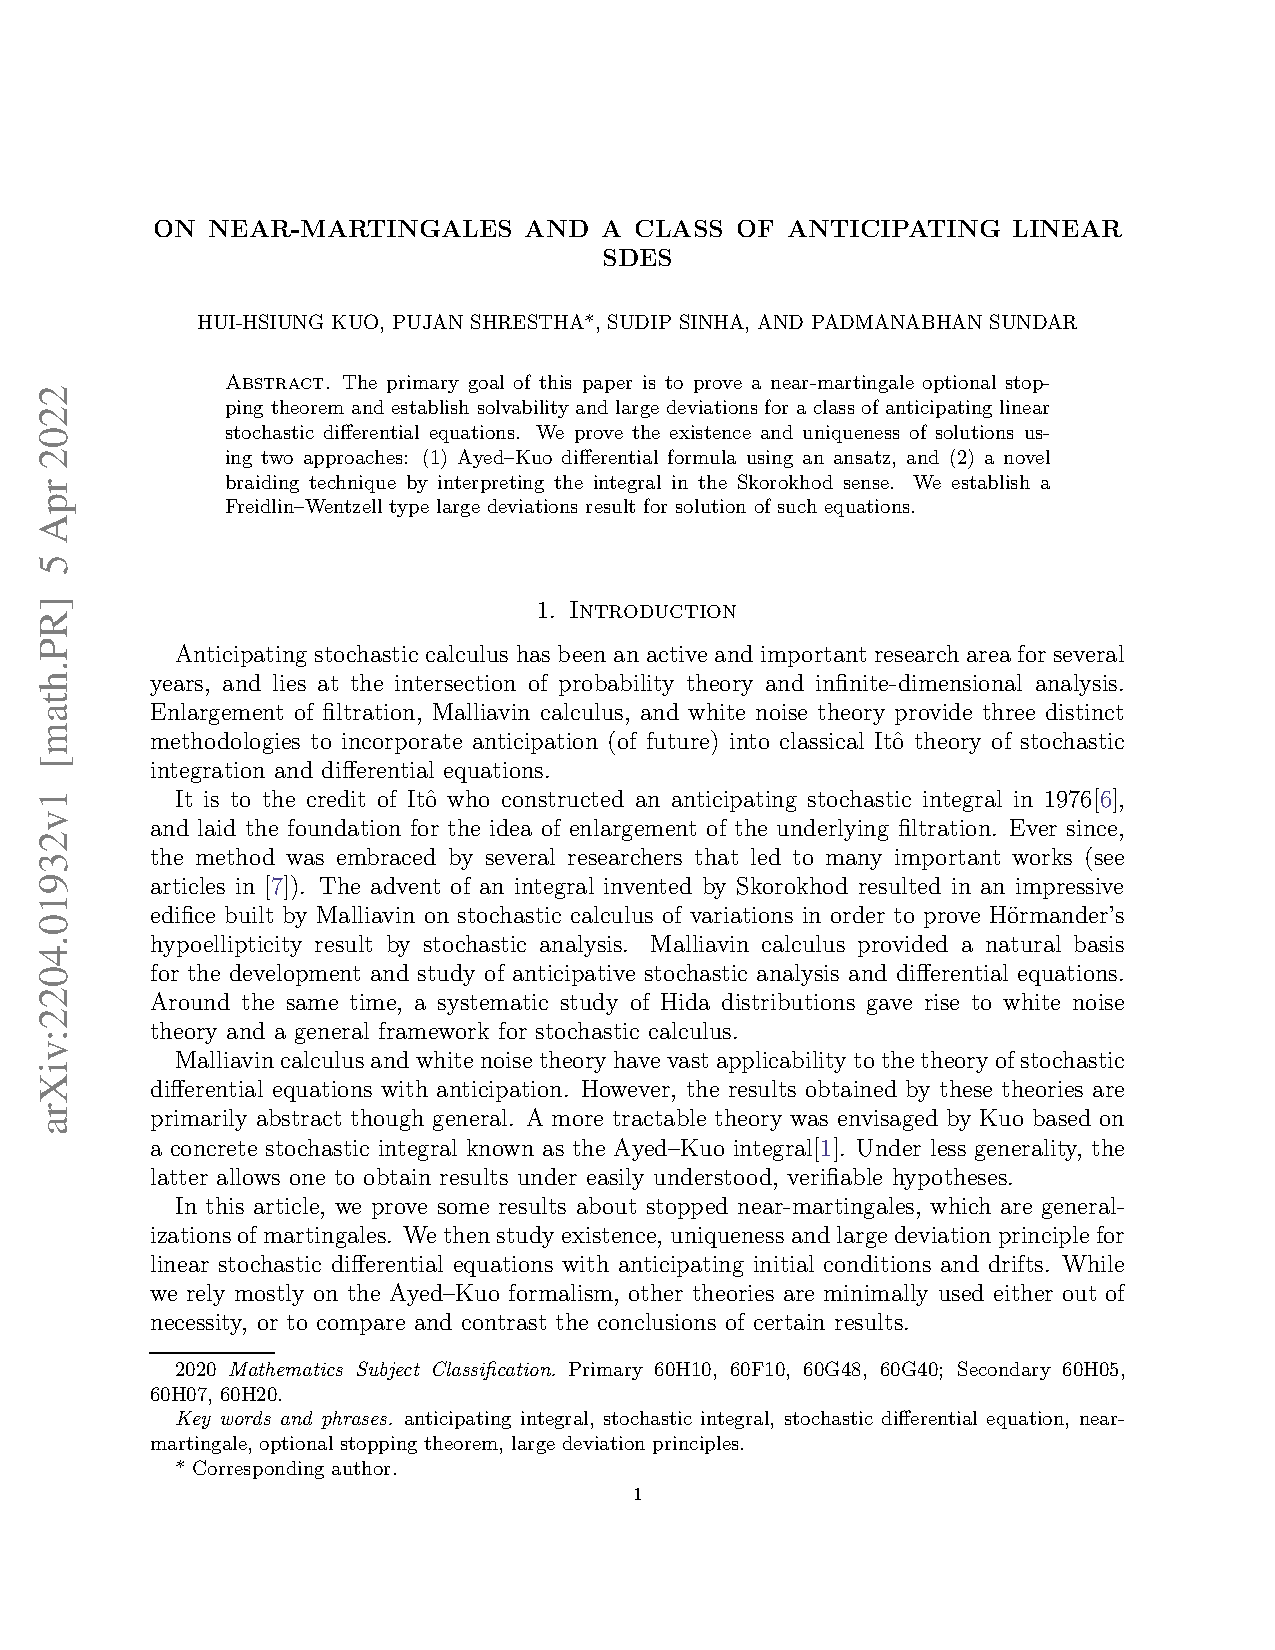
\includepdf[scale=0.875, offset=0 -4em, pages=-, pagecommand={\chapter*{Appendix. Copyright Information} \addcontentsline{toc}{chapter}{Appendix. Copyright Information} \section*{Copyright information for \fullcite{KuoShresthaSinhaSundar2022} used in \cref{chp:near-martingales,chp:solving_ALSDEs,chp:probabilistic_behavior}.}}]{misc/KuoShresthaSinhaSundar2022_p1.pdf}
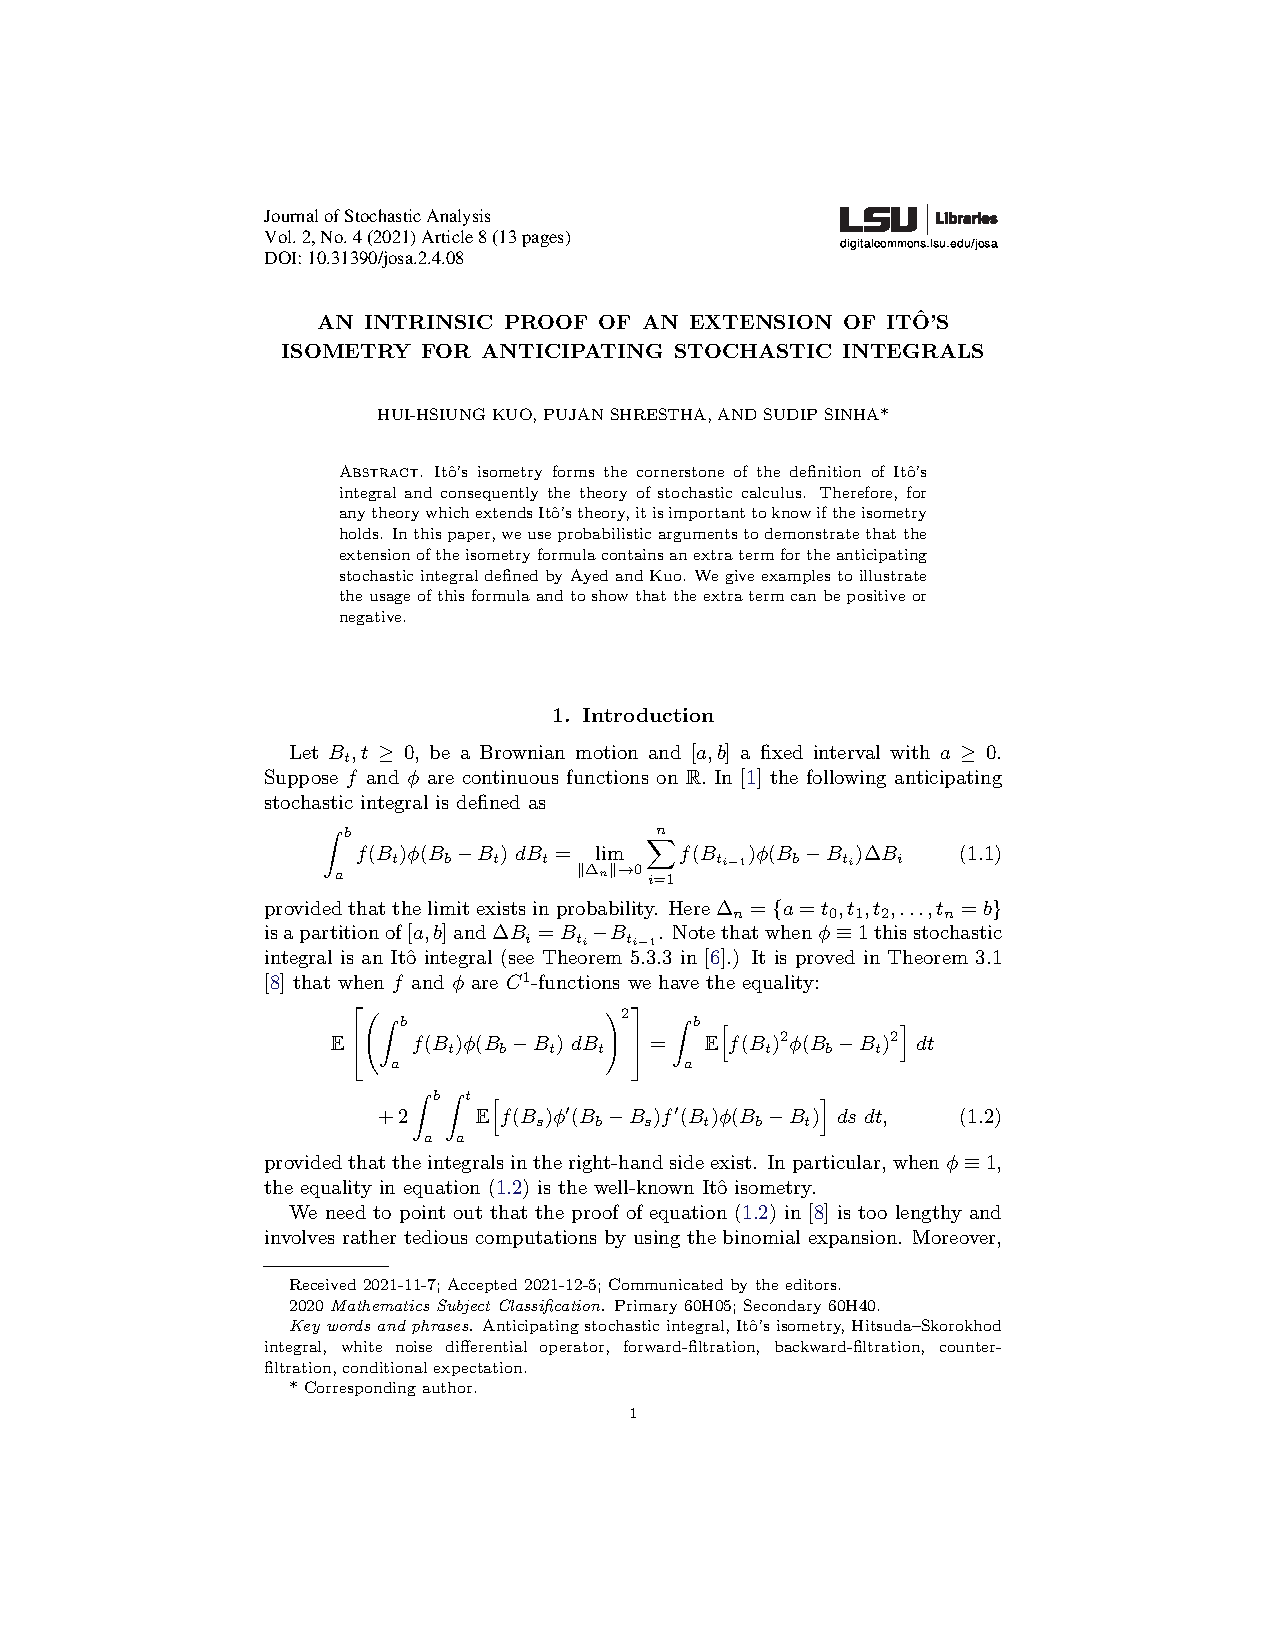
\includepdf[scale=1, offset=0 -4em, pages=-, pagecommand={\section*{Copyright information for \fullcite{KuoShresthaSinha2021isometry} used in \cref{chp:isometry}.}}]{misc/KuoShresthaSinha2021isometry_p1.pdf}
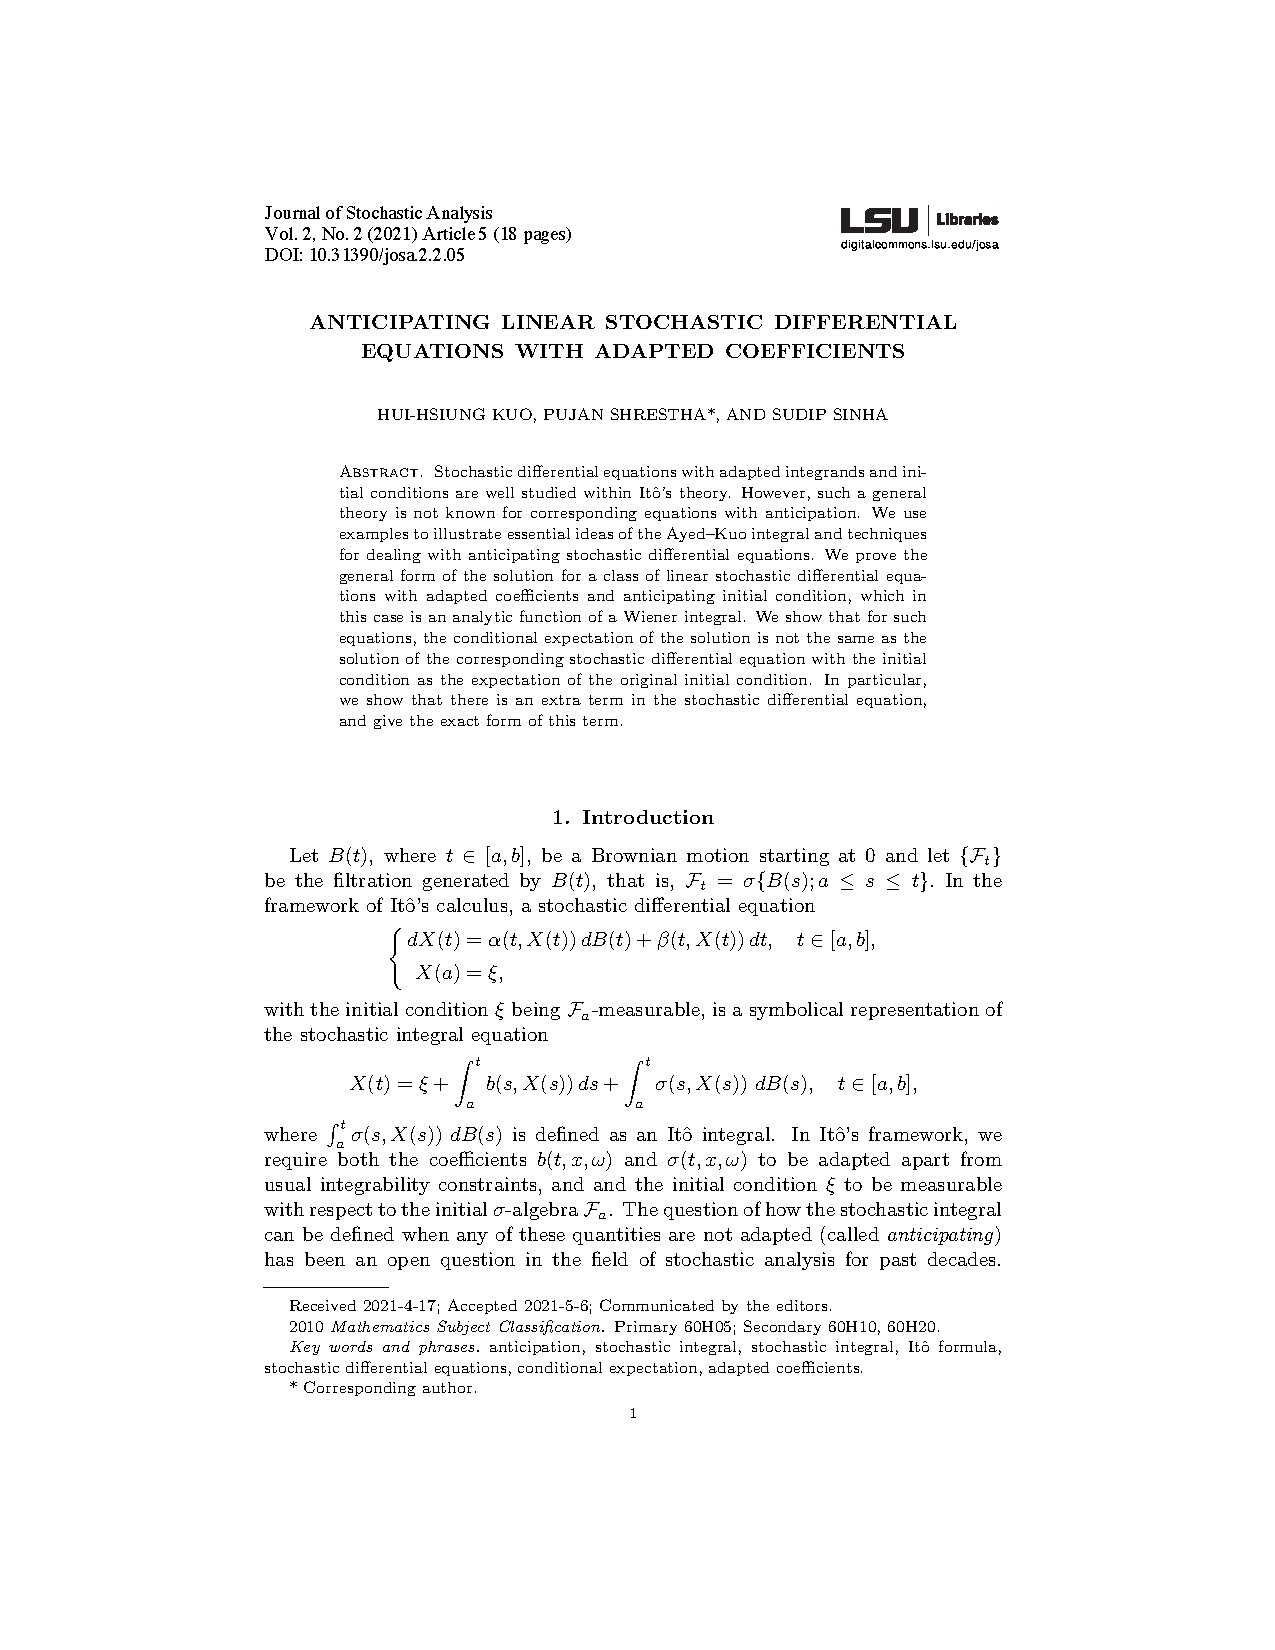
\includepdf[scale=1, offset=0 -4em, pages=-, pagecommand={\section*{Copyright information for \fullcite{KuoShresthaSinha2021conditional} used in \cref{chp:Ayed–Kuo_integral,chp:conditional}.}}]{misc/KuoShresthaSinha2021conditional_p1.pdf}
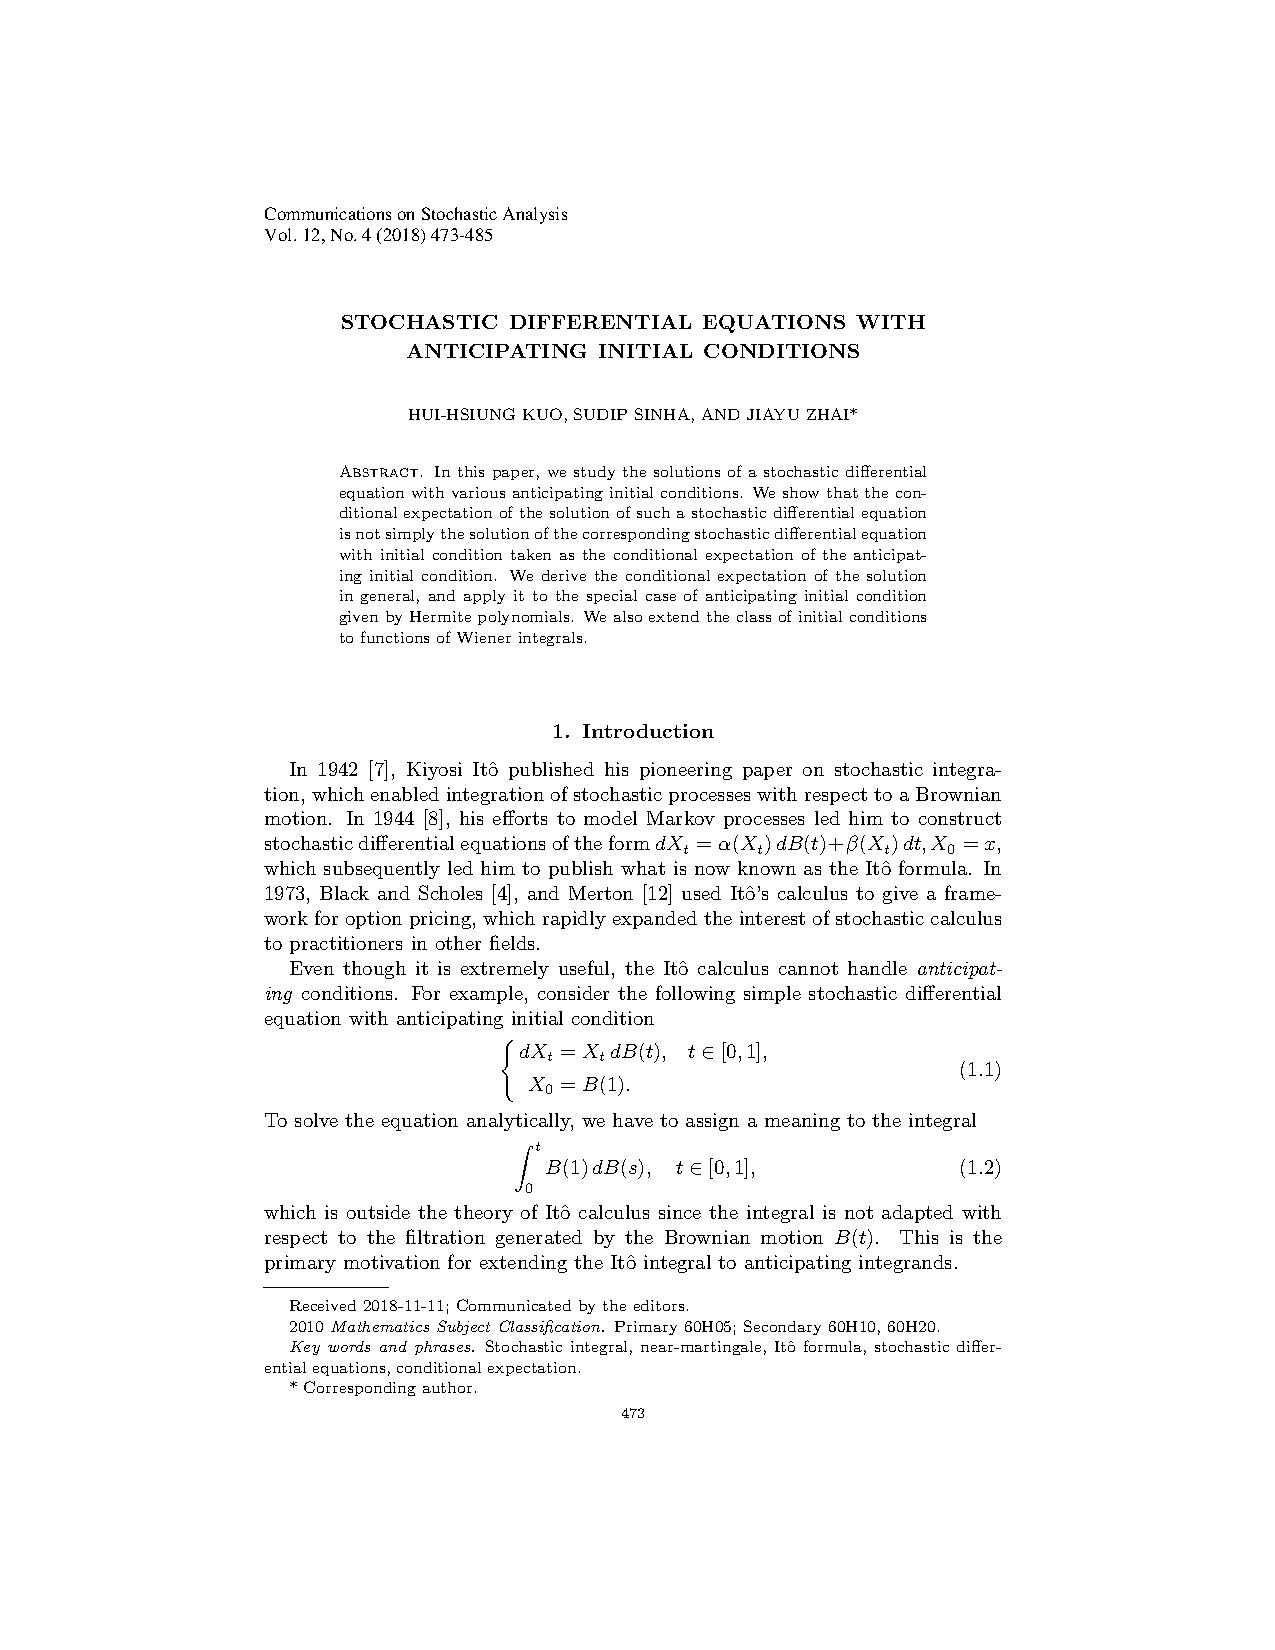
\includepdf[scale=1, offset=0 -4em, pages=-, pagecommand={\section*{Copyright information for \fullcite{KuoSinhaZhai2018} used in \cref{chp:Ayed–Kuo_integral}.}}]{misc/KuoSinhaZhai2018_p1.pdf}


%% After ``\backmatter'', subsequent \chapter commands produce unnumbered headings.
\backmatter

% \printindex

\printbibliography[heading=bibintoc]

\chapter{Vita}
% !TeX root = ../dissertation.tex

Born in a picturesque Indian town at the foothills of the Himalayas, Sudip Sinha grew up in Kolkata. After obtaining his bachelor's degree in chemical engineering from Birla Institute of Technology \& Science, Pilani in Goa, he worked for the Innovation Lab at Mu Sigma in Bengaluru. Subsequently, he joined the Erasmus Mundus master's program MathMods, studying mathematical modeling at the Università degli Studi dell'Aquila in Italy and Universität Hamburg in Germany.

He loves mathematics and is awestruck by its beauty and universality, and is inquisitive about its philosophical foundations. He has gradually developed a keen interest in teaching and writing expository articles, and desires to continue them throughout his life. After graduating, Sudip plans to join Amazon as an Applied Scientist.

Outside of academics, Sudip is an avid-reader, an amateur guitarist, and a self-confessed travel-addict who loves exploring various cultures and cuisines. Sudip finds peace in nature and hopes for an equitable and harmonious future for planet earth.


\end{document}
